%%%%%%%%%%%%%%%%%%%%%%%%%%%%%%%%%%%%%%%%%%%%%%%%%%%%%%%%%%%%%%%%%%%%%%%%%%%%%%%%%%%%%%%%%%%%%%%%%%%%%%%%%%%%%%%%%%%%%%%%%%%%%%%%%%%%%%%%%%%%%%%%%%%%%%%%%%%%%%%%%%%%%%%
%%%%%%%%%%%%%%%%%%%%%%%%%%%%%%%%%%%%%%%%%%%%%%%%%%%%%%%%%%%%%%%%%%%%%%%%%%%%%%%%%%%%%%%%%%%%%%%%%%%%%%%%%%%%%%%%%%%%%%%%%%%%%%%%%%%%%%%%%%%%%%%%%%%%%%%%%%%%%%%%%%%%%%%
\chapter{\texorpdfstring{A search for highly ionising, short tracks}{Appendix: \quad A search for highly ionising, short tracks}}
\section{Calibration of the silicon pixel detector}
\label{app:PixelCalibration}
In Fig.~\ref{fig:SigmaPixelCalibrationROCs}, the standard deviation of derived calibration factors of the ROCs within one module is depicted for all modules.
\begin{figure}[!b]
  \centering 
  \begin{tabular}{c}
    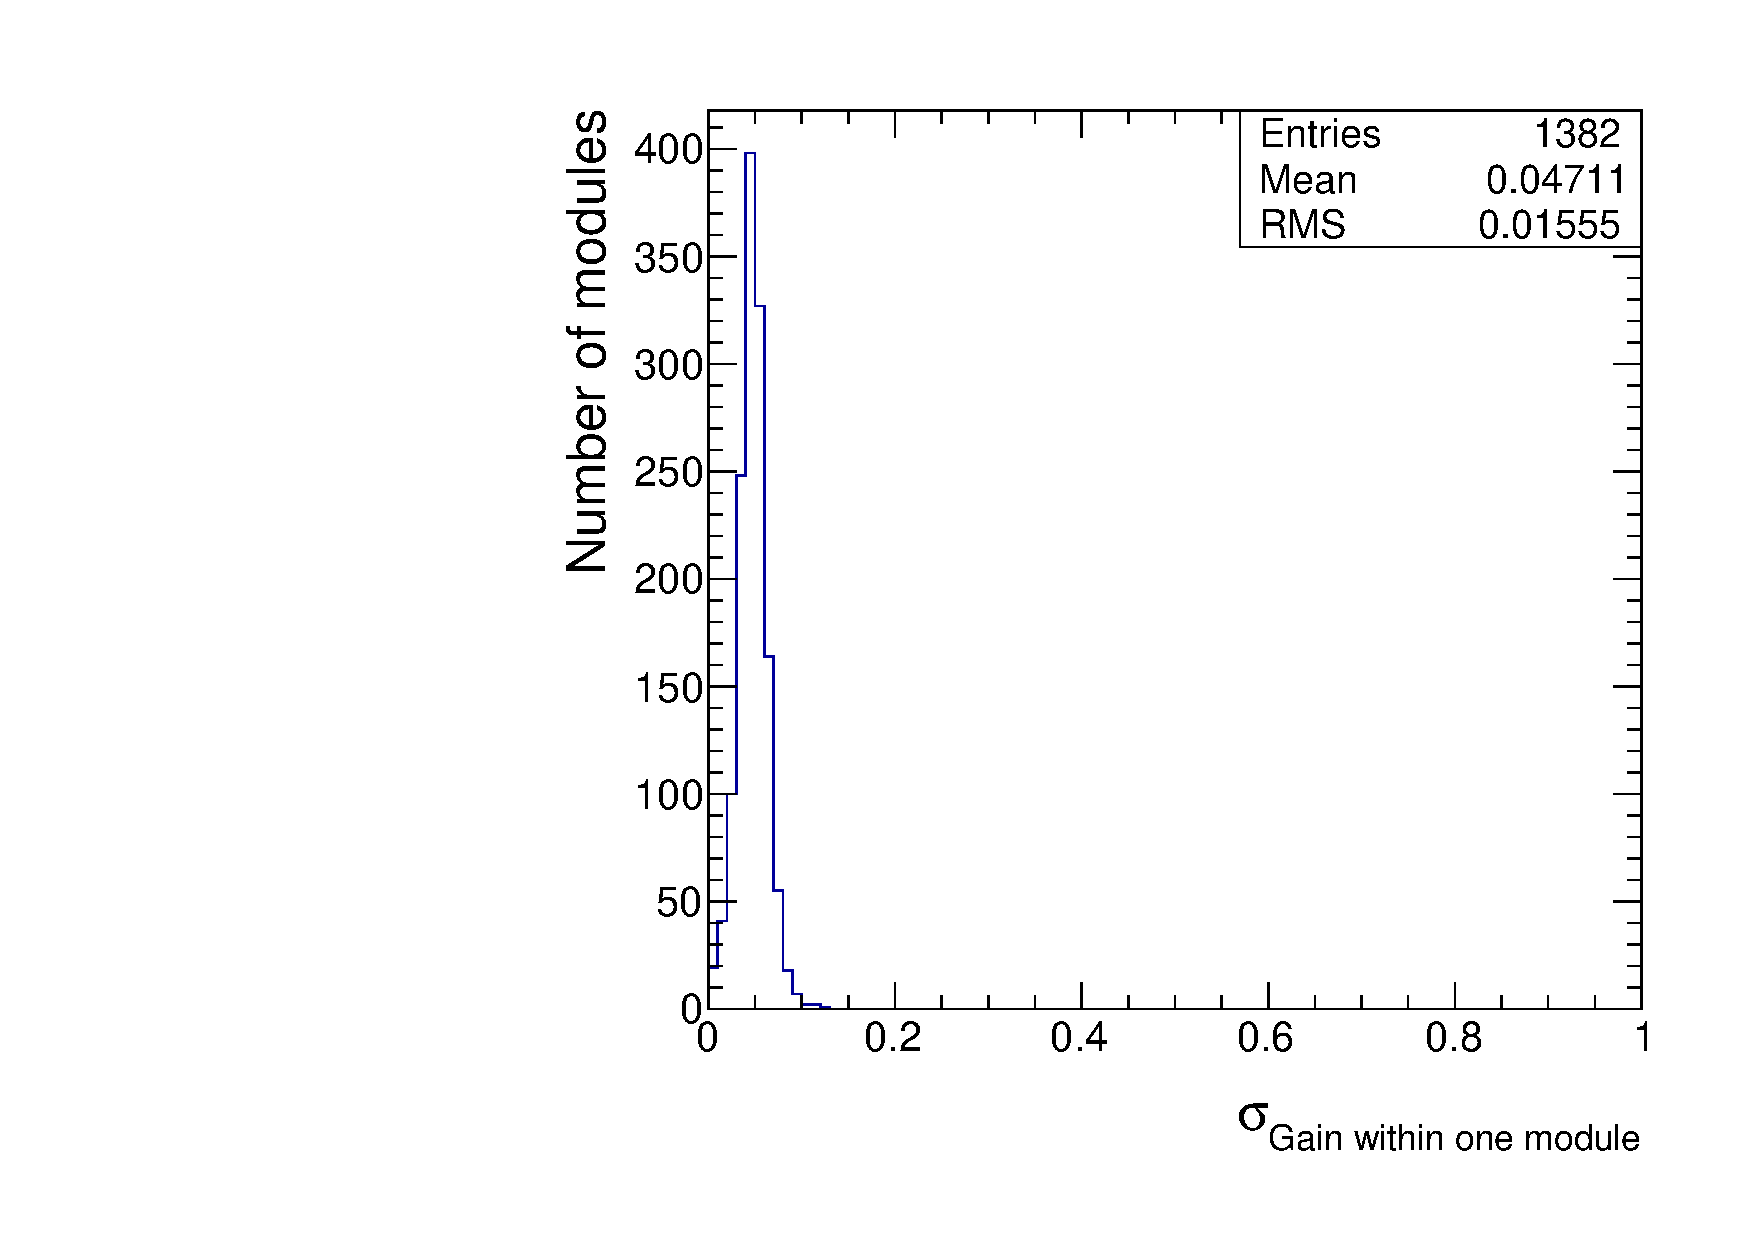
\includegraphics[width=0.33\textwidth]{figures/analysis_2/PixelCalibration/rmsOfROCs_N_0_AB_CL0} 
    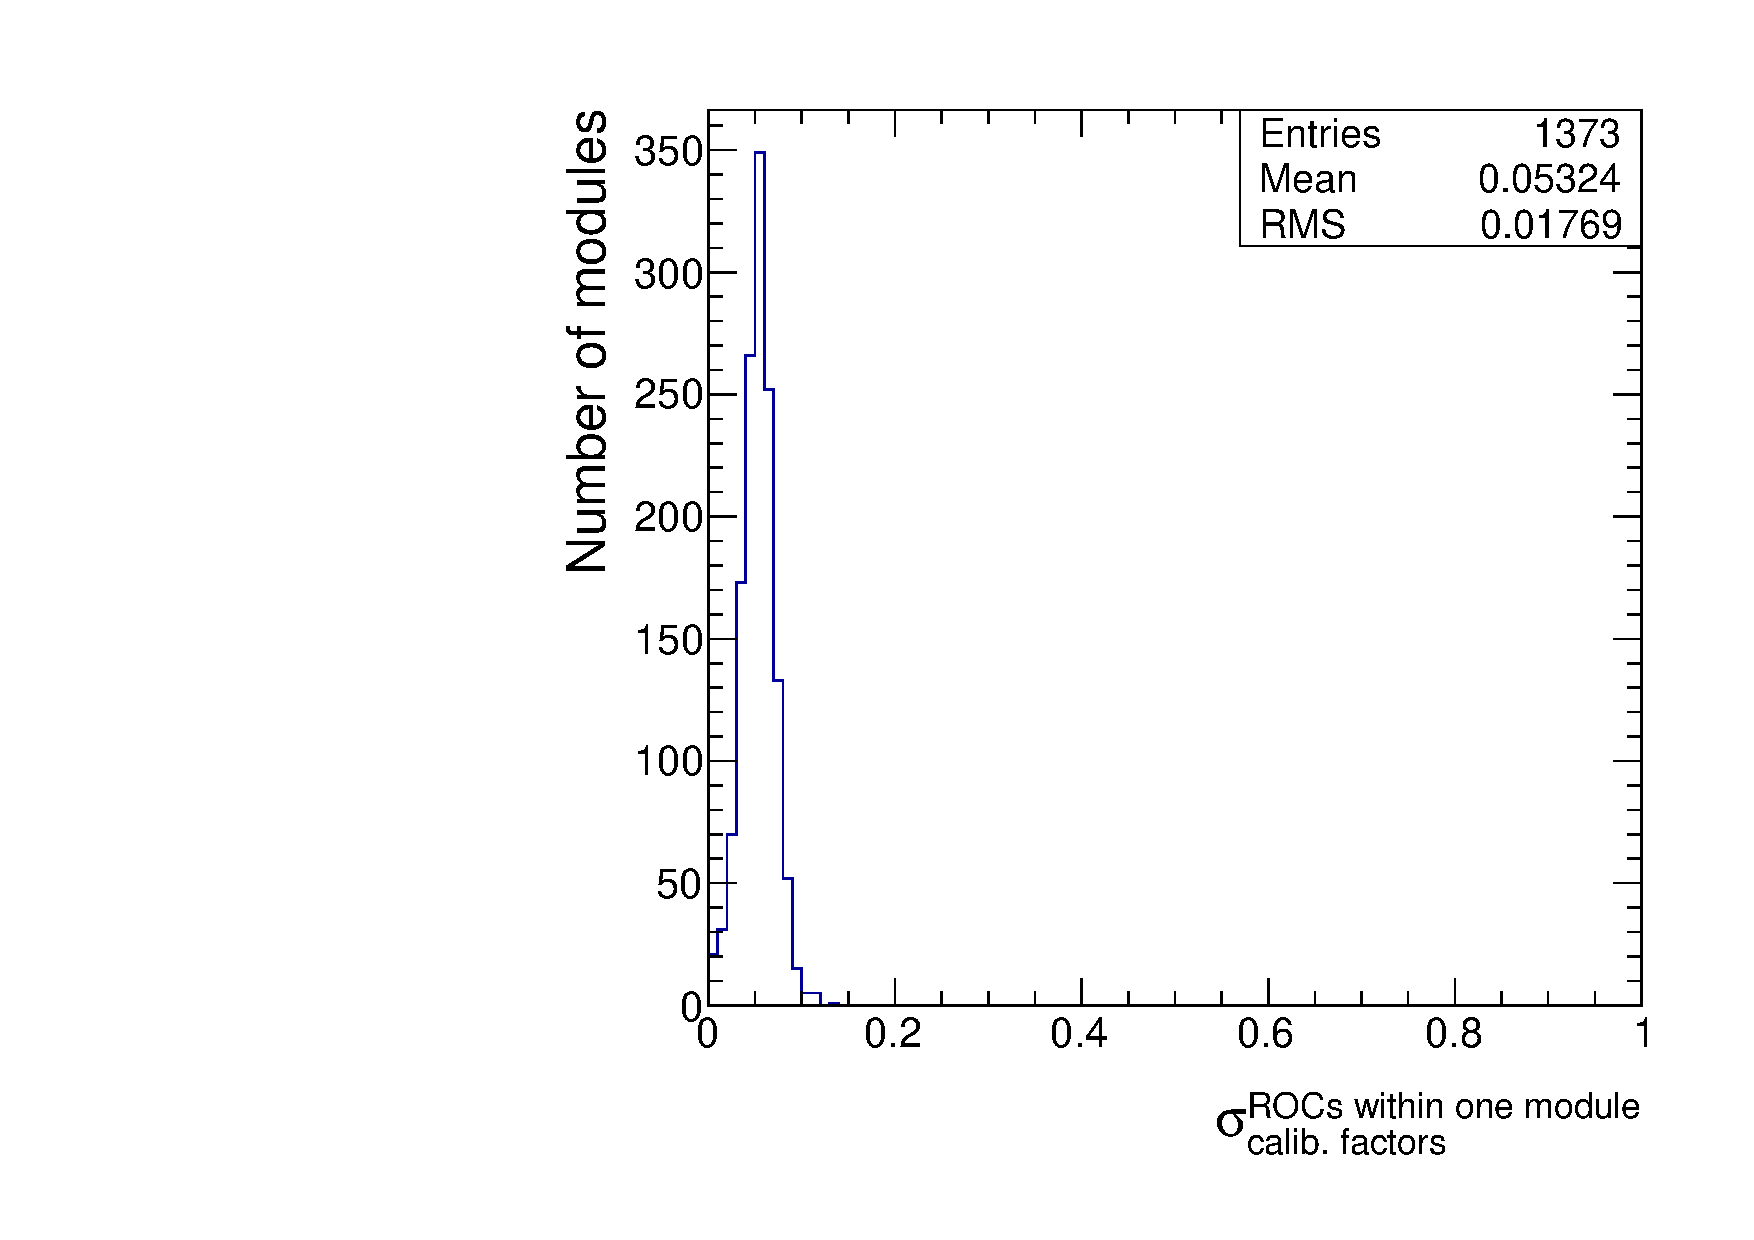
\includegraphics[width=0.33\textwidth]{figures/analysis_2/PixelCalibration/rmsOfROCs_N_0_C1_CL0} 
    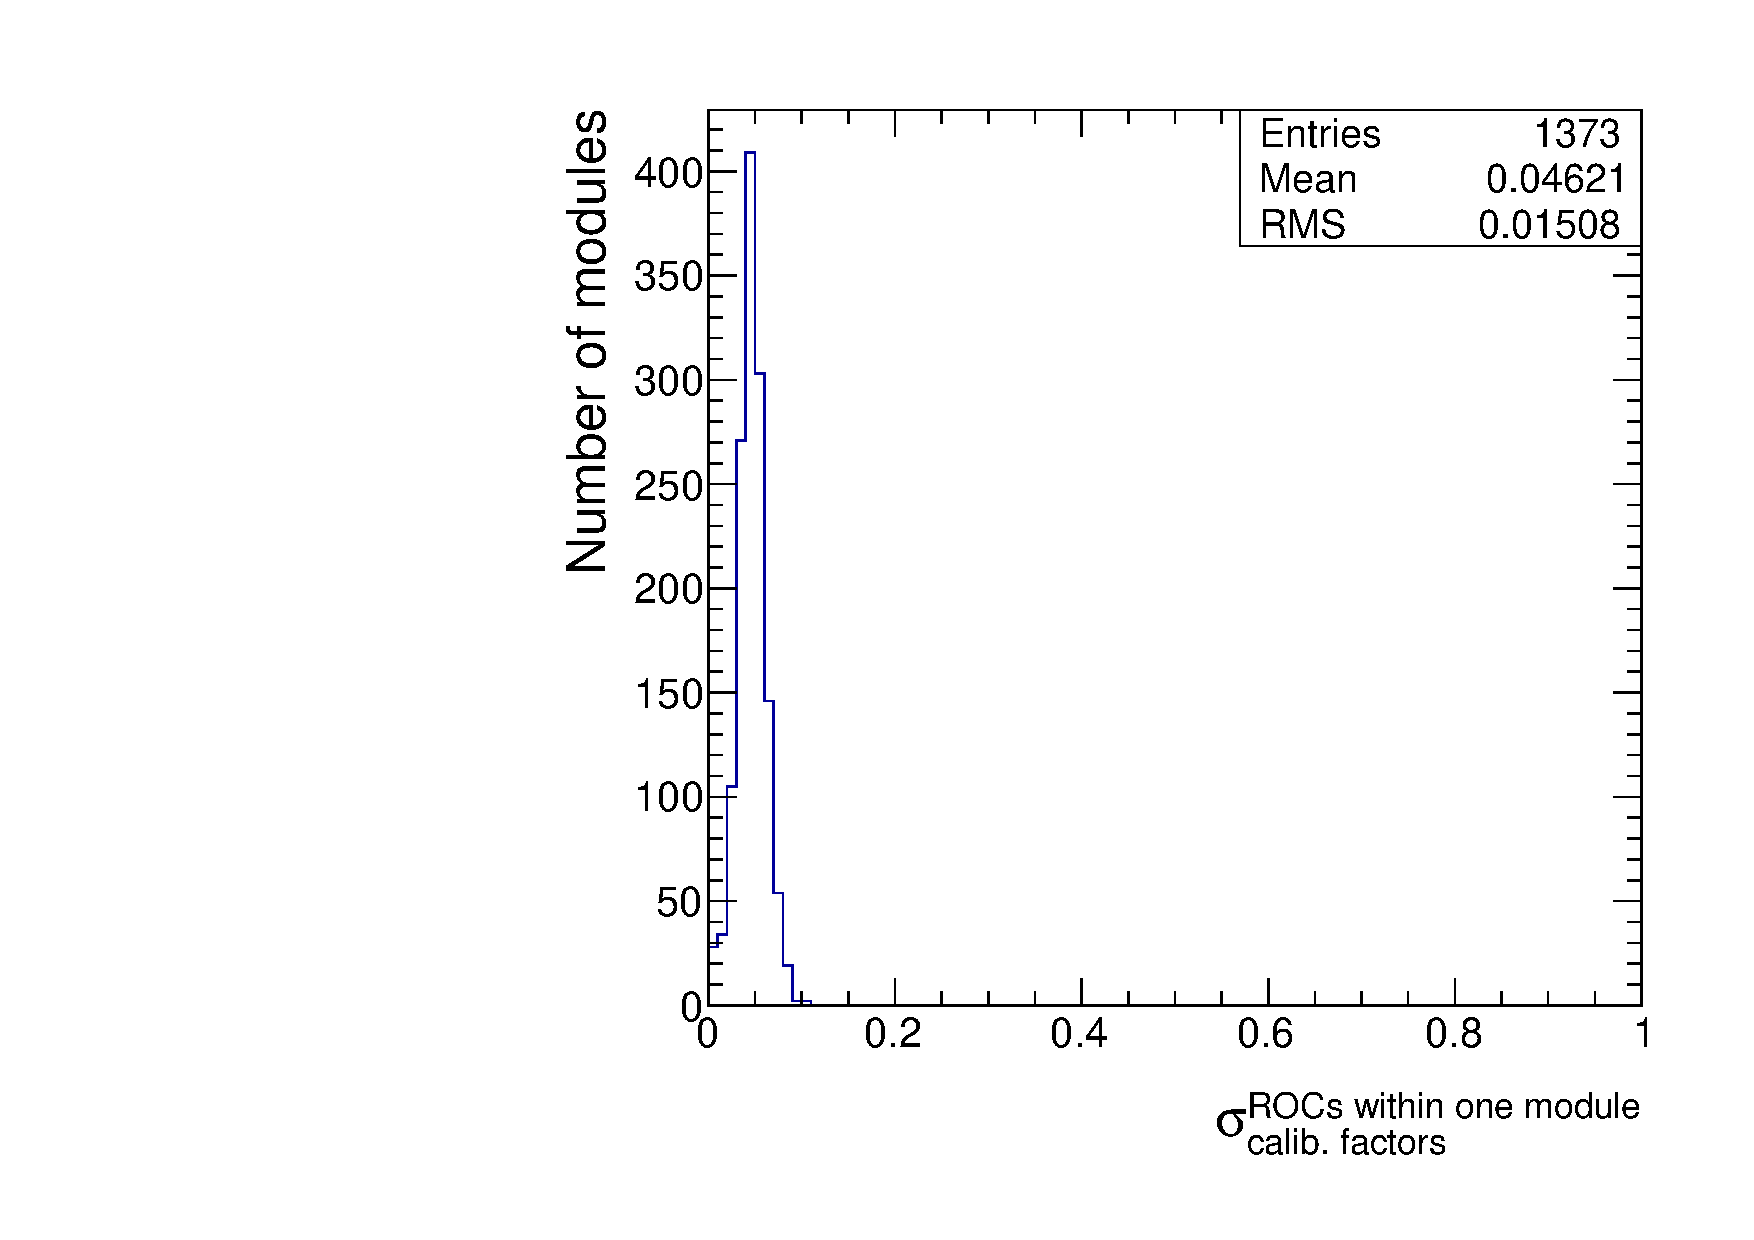
\includegraphics[width=0.33\textwidth]{figures/analysis_2/PixelCalibration/rmsOfROCs_N_0_C2_CL0} \\
    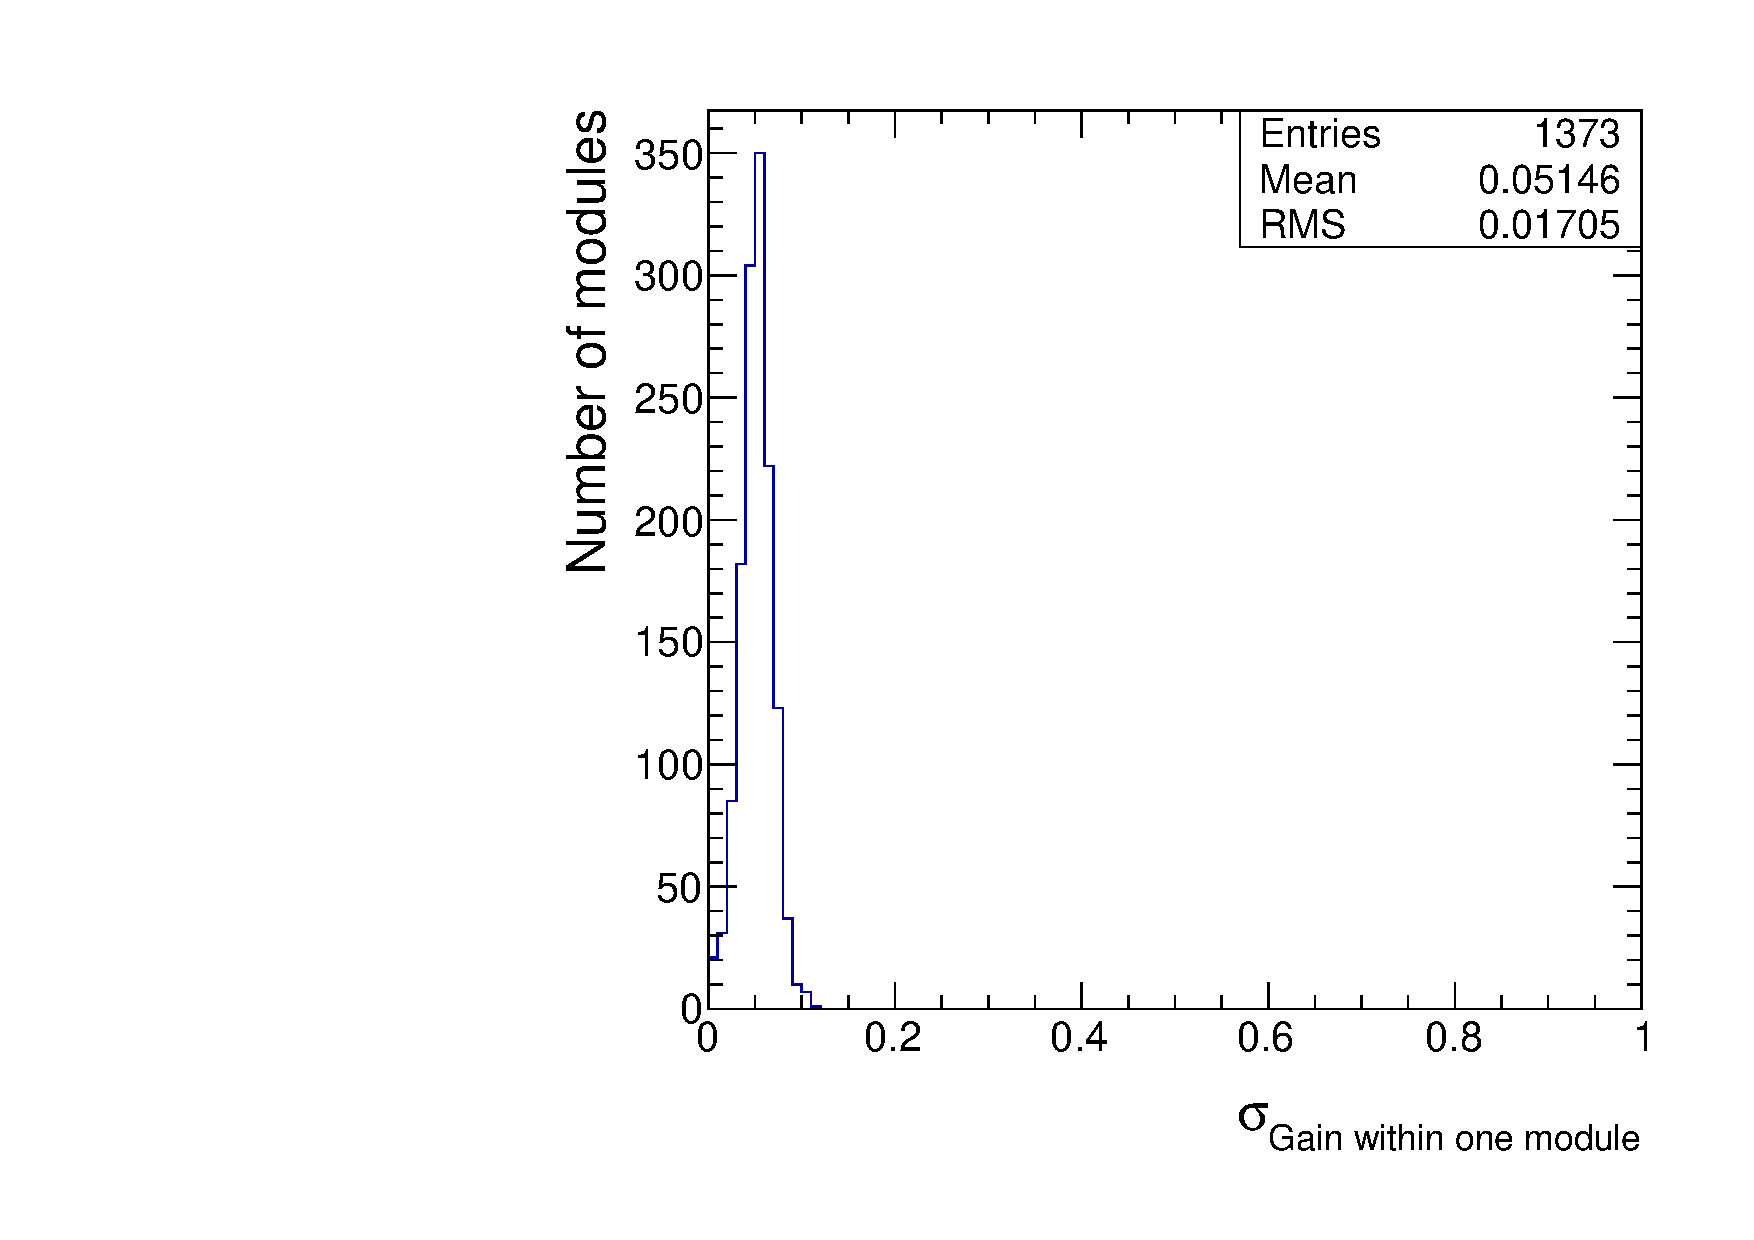
\includegraphics[width=0.33\textwidth]{figures/analysis_2/PixelCalibration/rmsOfROCs_N_0_D1_CL0} 
    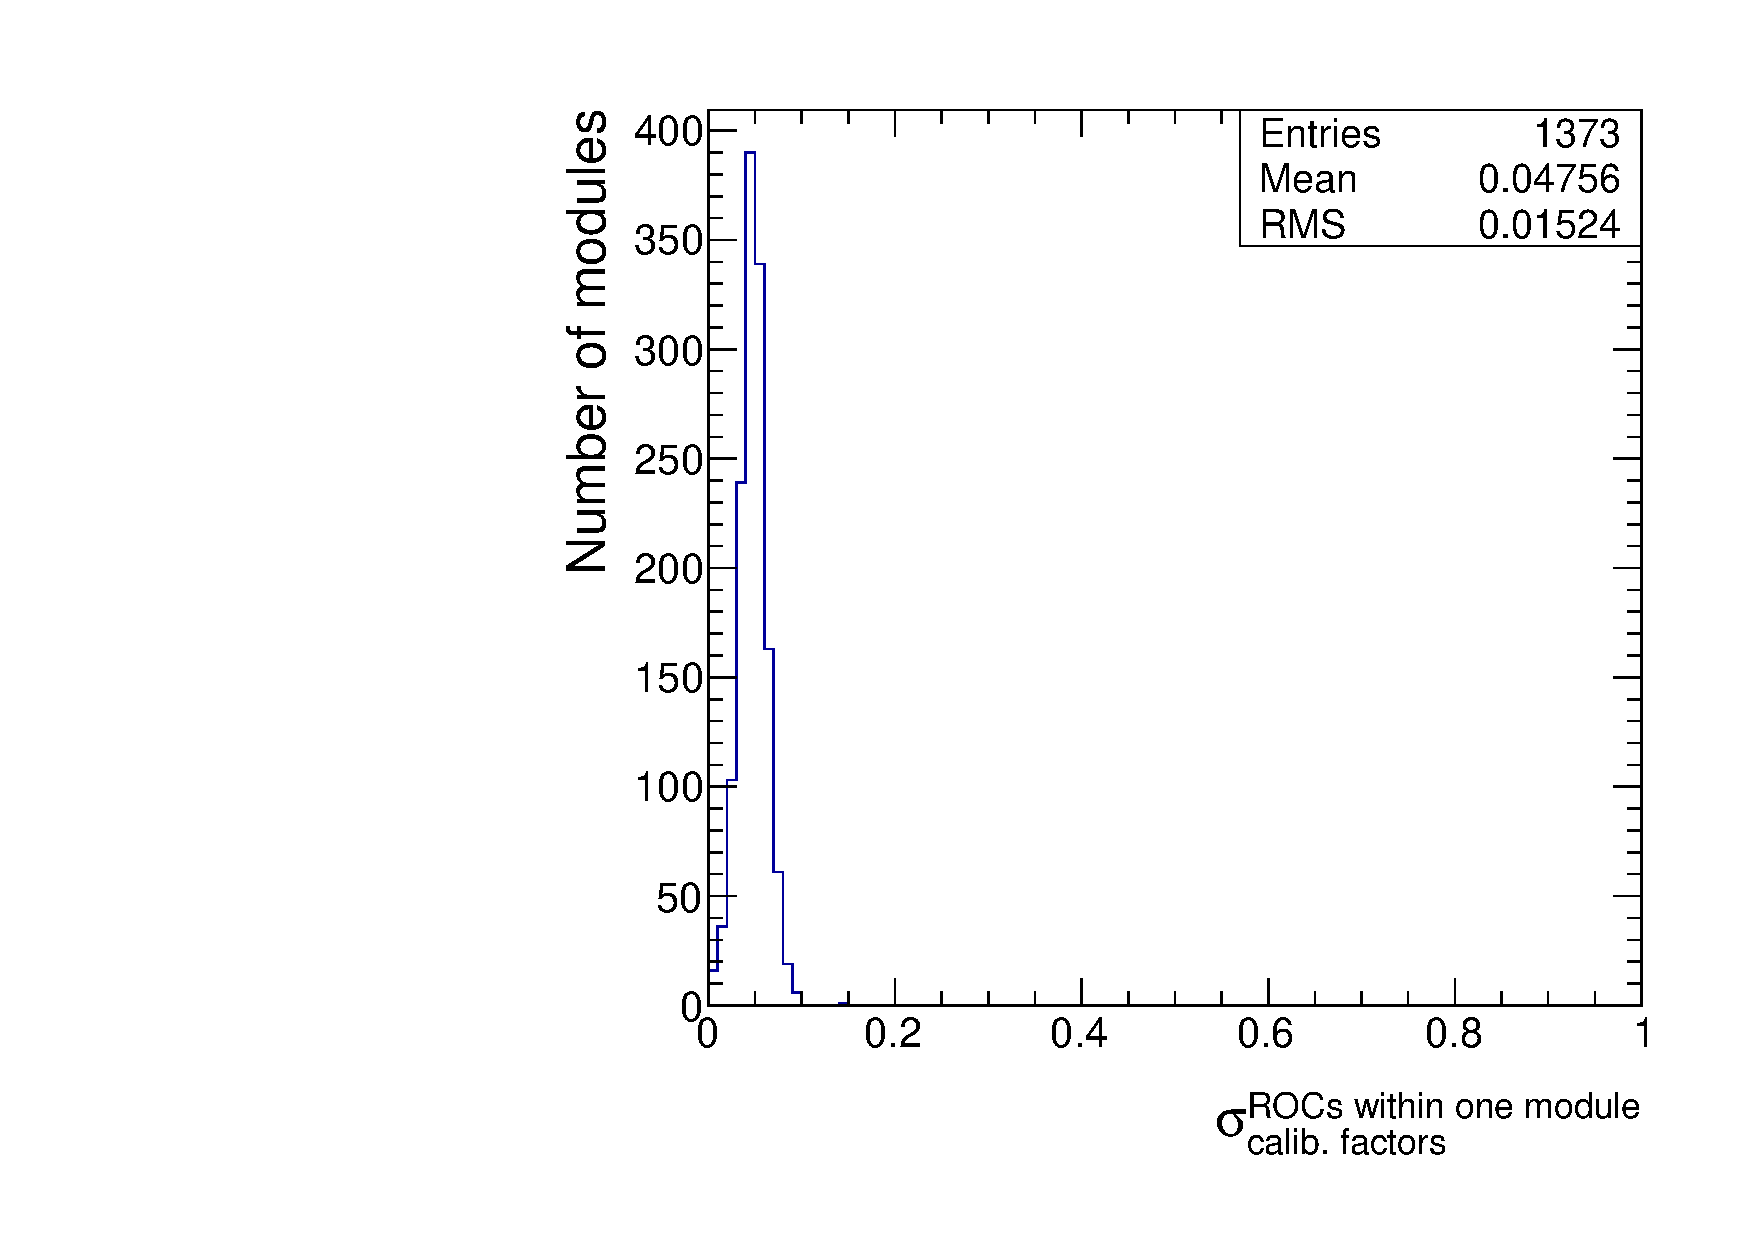
\includegraphics[width=0.33\textwidth]{figures/analysis_2/PixelCalibration/rmsOfROCs_N_0_D2_CL0} 
  \end{tabular}
  \caption{The standard deviation of the pixel calibration factors of all ROCs within one module for all five time intervals (first interval, second interval, .. from top left to bottom right).}
  \label{fig:SigmaPixelCalibrationROCs}
\end{figure} 
Most of the modules have a $\sigma_{\text{calib. factors}}$ around 5\%, but never worse than 10\%.
In~\cite{bib:Quertenmont_2010}, it was shown that the resolution of the inter-calibration of the silicon strip detector is limited to $\sim 10\%$.
This is expected to be of similar magnitude for the pixel tracker inter-calibration.
Therefore, the inter-calibration of ROCs within one module can be considered acceptable.

%%%%%%%%%%%%%%%%%%%%%%%%%%%%%%%%%%%%%%%%%%%%%%%%%%%%%%%%%%%%%%%%%%%%%%%%%%%%%%%%%%%%%%%%%%%%%%%%%%%%%%%%%%%%%%%%%%%%%%%%%%%%%%%%%%%%%%%%%%%%%%%%%%%%%%%%%%%%%%%%%%%%%%%
%%%%%%%%%%%%%%%%%%%%%%%%%%%%%%%%%%%%%%%%%%%%%%%%%%%%%%%%%%%%%%%%%%%%%%%%%%%%%%%%%%%%%%%%%%%%%%%%%%%%%%%%%%%%%%%%%%%%%%%%%%%%%%%%%%%%%%%%%%%%%%%%%%%%%%%%%%%%%%%%%%%%%%%
\clearpage
\FloatBarrier
\section{Lifetime reweighting}
\label{app:LifetimeReweighting}
The probability density function of a particle's proper lifetime for a sample generated with a particle's mean lifetime $\tau^{\text{gen}}$ is given by
\begin{equation*}
p \left( t \right) = \frac{1}{\tau^{\text{gen}}} \cdot \exp\left[ -\frac{t}{\tau^{\text{gen}}} \right].
\end{equation*}

After carrying out the lifetime reweighting procedure, the targeted p.d.f of the particle's new mean lifetime $\tau^{\text{target}}$ is given by
\begin{equation*}
p'  \left( t \right) = \frac{1}{\tau^{\text{target}}} \cdot \exp\left[ -\frac{t}{\tau^{\text{target}}} \right].
\end{equation*}
Thus, an event containing a particle with individual proper lifetime can be reweighted with the following weight
\begin{equation*}
\label{eq:reweight}
w = \frac{p'  \left( t \right)}{p \left( t \right)} = \frac{\tau^{\text{gen}}}{\tau^{\text{target}}} \cdot \exp\left[ \frac{t}{\tau^{\text{gen}}} - \frac{t}{\tau^{\text{target}}} \right].  %= \frac{\tau^{\text{gen}}}{\tau^{\text{target}}} \cdot \exp \left[ t \cdot \left( \frac{1}{\tau^{\text{gen}}} - \frac{1}{\tau^{\text{target}}} \right) \right] .
\end{equation*}
For more than one non-stable particle, the event weight is calculated by multiplying the weights of the single reweighting procedures.

%%%%%%%%%%%%%%%%%%%%%%%%%%%%%%%%%%%%%%%%%%%%%%%%%%%%%%%%%%%%%%%%%%%%%%%%%%%%%%%%%%%%%%%%%%%%%%%%%%%%%%%%%%%%%%%%%%%%%%%%%%%%%%%%%%%%%%%%%%%%%%%%%%%%%%%%%%%%%%%%%%%%%%%
%%%%%%%%%%%%%%%%%%%%%%%%%%%%%%%%%%%%%%%%%%%%%%%%%%%%%%%%%%%%%%%%%%%%%%%%%%%%%%%%%%%%%%%%%%%%%%%%%%%%%%%%%%%%%%%%%%%%%%%%%%%%%%%%%%%%%%%%%%%%%%%%%%%%%%%%%%%%%%%%%%%%%%%
\clearpage
\FloatBarrier
\section{Event yields for simulated samples and data}
\label{app:cutflow}


\renewcommand{\arraystretch}{1.35}
\begin{table}[!h]
%\begin{sideways}
\centering
\caption{Event yields after each selection step for various simulated background samples.}
\label{tab:CutflowMC}
\makebox[0.99\textwidth]{
\begin{tabular}{|l|c|c|c|c|}
\multicolumn{5}{c}{} \\
\toprule

Selection               &   \WJets  & \ttbarJets  & \Zlep & Multijet  \\
\midrule
After skim                                                                                & 9.16 $\cdot10^{7 }$ & 1.04 $\cdot10^{6 }$ & 2.21 $\cdot10^{7 }$ & 1.38 $\cdot10^{11}$ \\
Trigger                                                                                   & 4.31 $\cdot10^{6 }$ & 1.15 $\cdot10^{5 }$ & 4.23 $\cdot10^{3 }$ & 4.32 $\cdot10^{6 }$ \\
$\ptfirstjet>110\gev$                                                                     & 2.47 $\cdot10^{6 }$ & 7.17 $\cdot10^{4 }$ & 2.60 $\cdot10^{3 }$ & 2.75 $\cdot10^{6 }$ \\
$\met>100\gev$                                                                            & 1.89 $\cdot10^{6 }$ & 5.31 $\cdot10^{4 }$ & 6.26 $\cdot10^{2 }$ & 9.63 $\cdot10^{5 }$ \\
$\Delta\phi_{\text{max}} \left( \text{jet}_i, \text{jet}_j  \right)<2.7$                  & 1.11 $\cdot10^{6 }$ & 6.81 $\cdot10^{3 }$ & 1.32 $\cdot10^{2 }$ & 2.01 $\cdot10^{4 }$ \\
$\Delta\phi_{\text{max}} \left( \text{jet}_i, \met  \right)>0.5$                          & 1.11 $\cdot10^{6 }$ & 6.76 $\cdot10^{3 }$ & 1.32 $\cdot10^{2 }$ & 9.55 $\cdot10^{3 }$ \\
$\geq1$ track in the event with:                                                          
& 1.10 $\cdot10^{6 }$ & 6.75 $\cdot10^{3 }$ & 1.32 $\cdot10^{2 }$ & 9.55 $\cdot10^{3 }$ \\
high-purity                                                                               & 1.10 $\cdot10^{6 }$ & 6.74 $\cdot10^{3 }$ & 1.32 $\cdot10^{2 }$ & 9.55 $\cdot10^{3 }$ \\
$N_{\text{miss}}^{\text{middle}}=0$                                                       & 1.09 $\cdot10^{6 }$ & 6.72 $\cdot10^{3 }$ & 1.32 $\cdot10^{2 }$ & 9.55 $\cdot10^{3 }$ \\
$N_{\text{miss}}^{\text{inner}}=0$                                                        & 1.07 $\cdot10^{6 }$ & 6.70 $\cdot10^{3 }$ & 1.32 $\cdot10^{2 }$ & 9.55 $\cdot10^{3 }$ \\
$|d0|<0.02\cm$                                                                            & 1.07 $\cdot10^{6 }$ & 6.64 $\cdot10^{3 }$ & 1.32 $\cdot10^{2 }$ & 9.55 $\cdot10^{3 }$ \\
$|dz|<0.5\cm$                                                                             & 1.07 $\cdot10^{6 }$ & 6.63 $\cdot10^{3 }$ & 1.32 $\cdot10^{2 }$ & 9.55 $\cdot10^{3 }$ \\
$|\eta|<2.1$                                                                              & 1.03 $\cdot10^{6 }$ & 6.58 $\cdot10^{3 }$ & 1.32 $\cdot10^{2 }$ & 9.55 $\cdot10^{3 }$ \\
$\pt>20\gev$                                                                              & 8.14 $\cdot10^{5 }$ & 5.63 $\cdot10^{3 }$ & 1.32 $\cdot10^{2 }$ & 5.48 $\cdot10^{3 }$ \\
No $\mu$ within $\Delta R<0.15$                                                           & 7.15 $\cdot10^{5 }$ & 4.52 $\cdot10^{3 }$ & 1.32 $\cdot10^{2 }$ & 5.48 $\cdot10^{3 }$ \\
No e within $\Delta R<0.15$                                                               & 6.69 $\cdot10^{5 }$ & 3.67 $\cdot10^{3 }$ & 7.86 $\cdot10^{1 }$ & 5.48 $\cdot10^{3 }$ \\
No $\tau$ within $\Delta R<0.15$                                                          & 6.62 $\cdot10^{5 }$ & 3.61 $\cdot10^{3 }$ & 7.86 $\cdot10^{1 }$ & 5.47 $\cdot10^{3 }$ \\
No jet within $\Delta R<0.5$                                                              & 1.18 $\cdot10^{3 }$ & 1.44 $\cdot10^{1 }$ & 1.09 $\cdot10^{1 }$ & 0.00 $\cdot10^{0 }$ \\
\makecell[l]{Not within $\Delta R<0.05$ of \\\hfill a dead/noisy ECAL cell}               & 7.25 $\cdot10^{2 }$ & 8.02 $\cdot10^{0 }$ & 0.00 $\cdot10^{0 }$ & 0.00 $\cdot10^{0 }$ \\
Not within an ECAL  intermodule gap                                                       & 7.15 $\cdot10^{2 }$ & 8.02 $\cdot10^{0 }$ & 0.00 $\cdot10^{0 }$ & 0.00 $\cdot10^{0 }$ \\
Not within $1.42<|\eta|<1.65$                                                             & 5.89 $\cdot10^{2 }$ & 6.53 $\cdot10^{0 }$ & 0.00 $\cdot10^{0 }$ & 0.00 $\cdot10^{0 }$ \\
Not within $\Delta R<0.25$ to a bad CSC                                                   & 5.02 $\cdot10^{2 }$ & 5.88 $\cdot10^{0 }$ & 0.00 $\cdot10^{0 }$ & 0.00 $\cdot10^{0 }$ \\
$\sum \limits_{\Delta R < 0.3} \pt^{\text{trk}}/\pt^{\text{cand}} - 1 < 0.1$              & 4.46 $\cdot10^{2 }$ & 4.78 $\cdot10^{0 }$ & 0.00 $\cdot10^{0 }$ & 0.00 $\cdot10^{0 }$ \\
$\ecalo<5\gev$                                                                            & 3.19 $\cdot10^{1 }$ & 0.67 $\cdot10^{0 }$ & 0.00 $\cdot10^{0 }$ & 0.00 $\cdot10^{0 }$ \\
\midrule
$\pt>30\gev$                                                                              & 3.19 $\cdot10^{1 }$ & 0.67 $\cdot10^{0 }$ & 0.00 $\cdot10^{0 }$ & 0.00 $\cdot10^{0 }$ \\
$\ias>0.05$                                                                               & 1.68 $\cdot10^{1 }$ & 0.16 $\cdot10^{0 }$ & 0.00 $\cdot10^{0 }$ & 0.00 $\cdot10^{0 }$ \\
\bottomrule
\end{tabular}}
%\end{sideways}
\end{table}  
%\end{landscape}

\renewcommand{\arraystretch}{1.35}
\begin{table}[!h]
%\begin{sideways}
\centering
\caption{Event yields after each selection step for various signal models.}
\label{tab:CutflowSignal}
\makebox[0.99\textwidth]{
\begin{tabular}{|l|c|c|c|c|}
\multicolumn{5}{c}{} \\
\toprule

\multirow{2}{*}{Selection}                                              &   m=100\gev          &   m=100\gev          &   m=500\gev          &   m=500\gev          \\
                                                                        &   $c\tau$=10\cm      &   $c\tau$=100\cm     &   $c\tau$=10\cm      &   $c\tau$=100\cm      \\
\midrule
Total                                                                                     & 3.41 $\cdot10^{5 }$ & 3.41 $\cdot10^{5 }$ & 3.46 $\cdot10^{2 }$ & 3.46 $\cdot10^{2 }$ \\
Trigger                                                                                   & 1.55 $\cdot10^{4 }$ & 1.49 $\cdot10^{4 }$ & 4.62 $\cdot10^{1 }$ & 4.61 $\cdot10^{1 }$ \\
$\ptfirstjet>110\gev$                                                                     & 1.10 $\cdot10^{4 }$ & 1.04 $\cdot10^{4 }$ & 3.64 $\cdot10^{1 }$ & 3.58 $\cdot10^{1 }$ \\
$\met>100\gev$                                                                            & 1.09 $\cdot10^{4 }$ & 9.82 $\cdot10^{3 }$ & 3.63 $\cdot10^{1 }$ & 3.56 $\cdot10^{1 }$ \\
$\Delta\phi_{\text{max}} \left( \text{jet}_i, \text{jet}_j  \right)<2.7$                  & 7.90 $\cdot10^{3 }$ & 7.03 $\cdot10^{3 }$ & 2.76 $\cdot10^{1 }$ & 2.71 $\cdot10^{1 }$ \\
$\Delta\phi_{\text{max}} \left( \text{jet}_i, \met  \right)>0.5$                          & 7.90 $\cdot10^{3 }$ & 6.98 $\cdot10^{3 }$ & 2.76 $\cdot10^{1 }$ & 2.70 $\cdot10^{1 }$ \\
$\geq1$ track in the event with:                                                          
& 3.12 $\cdot10^{3 }$ & 5.74 $\cdot10^{3 }$ & 5.73 $\cdot10^{0 }$ & 2.13 $\cdot10^{1 }$ \\
high-purity                                                                               & 2.90 $\cdot10^{3 }$ & 5.66 $\cdot10^{3 }$ & 5.24 $\cdot10^{0 }$ & 2.08 $\cdot10^{1 }$ \\
$N_{\text{miss}}^{\text{middle}}=0$                                                       & 2.86 $\cdot10^{3 }$ & 5.46 $\cdot10^{3 }$ & 5.23 $\cdot10^{0 }$ & 2.02 $\cdot10^{1 }$ \\
$N_{\text{miss}}^{\text{inner}}=0$                                                        & 2.85 $\cdot10^{3 }$ & 5.41 $\cdot10^{3 }$ & 5.22 $\cdot10^{0 }$ & 2.01 $\cdot10^{1 }$ \\
$|d0|<0.02\cm$                                                                            & 2.80 $\cdot10^{3 }$ & 5.39 $\cdot10^{3 }$ & 5.07 $\cdot10^{0 }$ & 1.99 $\cdot10^{1 }$ \\
$|dz|<0.5\cm$                                                                             & 2.79 $\cdot10^{3 }$ & 5.38 $\cdot10^{3 }$ & 5.07 $\cdot10^{0 }$ & 1.99 $\cdot10^{1 }$ \\
$|\eta|<2.1$                                                                              & 2.63 $\cdot10^{3 }$ & 4.98 $\cdot10^{3 }$ & 5.01 $\cdot10^{0 }$ & 1.91 $\cdot10^{1 }$ \\
$\pt>20\gev$                                                                              & 2.54 $\cdot10^{3 }$ & 4.93 $\cdot10^{3 }$ & 4.72 $\cdot10^{0 }$ & 1.88 $\cdot10^{1 }$ \\
No $\mu$ within $\Delta R<0.15$                                                           & 2.54 $\cdot10^{3 }$ & 4.65 $\cdot10^{3 }$ & 4.72 $\cdot10^{0 }$ & 1.86 $\cdot10^{1 }$ \\
No e within $\Delta R<0.15$                                                               & 2.54 $\cdot10^{3 }$ & 4.65 $\cdot10^{3 }$ & 4.72 $\cdot10^{0 }$ & 1.86 $\cdot10^{1 }$ \\
No $\tau$ within $\Delta R<0.15$                                                          & 2.54 $\cdot10^{3 }$ & 4.64 $\cdot10^{3 }$ & 4.72 $\cdot10^{0 }$ & 1.86 $\cdot10^{1 }$ \\
No jet within $\Delta R<0.5$                                                              & 2.53 $\cdot10^{3 }$ & 4.60 $\cdot10^{3 }$ & 4.63 $\cdot10^{0 }$ & 1.82 $\cdot10^{1 }$ \\
\makecell[l]{Not within $\Delta R<0.05$ of \\\hfill a dead/noisy ECAL cell}               & 2.32 $\cdot10^{3 }$ & 4.26 $\cdot10^{3 }$ & 4.19 $\cdot10^{0 }$ & 1.69 $\cdot10^{1 }$ \\
Not within an ECAL  intermodule gap                                                       & 2.30 $\cdot10^{3 }$ & 4.23 $\cdot10^{3 }$ & 4.16 $\cdot10^{0 }$ & 1.67 $\cdot10^{1 }$ \\
Not within $1.42<|\eta|<1.65$                                                             & 2.09 $\cdot10^{3 }$ & 3.88 $\cdot10^{3 }$ & 3.94 $\cdot10^{0 }$ & 1.56 $\cdot10^{1 }$ \\
Not within $\Delta R<0.25$ to a bad CSC                                                   & 1.98 $\cdot10^{3 }$ & 3.67 $\cdot10^{3 }$ & 3.82 $\cdot10^{0 }$ & 1.50 $\cdot10^{1 }$ \\
$\sum \limits_{\Delta R < 0.3} \pt^{\text{trk}}/\pt^{\text{cand}} - 1 < 0.1$              & 1.96 $\cdot10^{3 }$ & 3.64 $\cdot10^{3 }$ & 3.78 $\cdot10^{0 }$ & 1.49 $\cdot10^{1 }$ \\
$\ecalo<5\gev$                                                                            & 1.66 $\cdot10^{3 }$ & 3.05 $\cdot10^{3 }$ & 3.38 $\cdot10^{0 }$ & 1.26 $\cdot10^{1 }$ \\
\midrule
$\pt>30\gev$                                                                              & 1.53 $\cdot10^{3 }$ & 2.98 $\cdot10^{3 }$ & 2.94 $\cdot10^{0 }$ & 1.23 $\cdot10^{1 }$ \\
$\ias>0.05$                                                                               & 8.18 $\cdot10^{2 }$ & 1.47 $\cdot10^{3 }$ & 2.52 $\cdot10^{0 }$ & 1.07 $\cdot10^{1 }$ \\
\bottomrule
\end{tabular}}
%\end{sideways}
\end{table}  
%\end{landscape}

\renewcommand{\arraystretch}{1.35}
\begin{table}[!h]
%\begin{sideways}
\centering
\caption{Observed event yield after each selection step in data.}
\label{tab:CutflowData}
\makebox[0.99\textwidth]{
\begin{tabular}{|l|c|}
\multicolumn{2}{c}{} \\
\toprule

Selection                                                                                 &   MET dataset               \\

\midrule

After skim                                                                                & 1.07 $\cdot10^{7 }$ \\
Trigger                                                                                   & 1.07 $\cdot10^{7 }$ \\
$\ptfirstjet>110\gev$                                                                     & 6.82 $\cdot10^{6 }$ \\
$\met>100\gev$                                                                            & 3.94 $\cdot10^{6 }$ \\
$\Delta\phi_{\text{max}} \left( \text{jet}_i, \text{jet}_j  \right)<2.7$                     & 1.39 $\cdot10^{6 }$ \\
$\Delta\phi_{\text{max}} \left( \text{jet}_{1,2}, \met  \right)>0.5$                             & 1.38 $\cdot10^{6 }$ \\
$\geq1$ track in the event with:                                 &\\                         
reconstructed trk                                                                         & 1.37 $\cdot10^{6 }$ \\
high-purity                                                                               & 1.36 $\cdot10^{6 }$ \\
$N_{\text{miss}}^{\text{middle}}=0$                                                              & 1.34 $\cdot10^{6 }$ \\
$N_{\text{miss}}^{\text{inner}}=0$                                                               & 1.31 $\cdot10^{6 }$ \\
$|d0|<0.02\cm$                                                                            & 1.30 $\cdot10^{6 }$ \\
$|dz|<0.5\cm$                                                                             & 1.30 $\cdot10^{6 }$ \\
$|\eta|<2.1$                                                                              & 1.26 $\cdot10^{6 }$ \\
$\pt>20\gev$                                                                              & 9.51 $\cdot10^{5 }$ \\
No $\mu$ within $\Delta R<0.15$                                                           & 8.40 $\cdot10^{5 }$ \\
No e within $\Delta R<0.15$                                                               & 8.01 $\cdot10^{5 }$ \\
No $\tau$ within $\Delta R<0.15$                                                          & 7.95 $\cdot10^{5 }$ \\
No jet within $\Delta R<0.5$                                                              & 1.75 $\cdot10^{3 }$ \\
\makecell[l]{Not within $\Delta R<0.05$ of \\\hfill a dead/noisy ECAL cell}               & 9.11 $\cdot10^{2 }$ \\
Not within an ECAL  intermodule gap                                                       & 9.06 $\cdot10^{2 }$ \\
Not within $1.42<|\eta|<1.65$                                                             & 7.33 $\cdot10^{2 }$ \\
Not within $\Delta R<0.25$ to a bad CSC                                                   & 6.16 $\cdot10^{2 }$ \\
$\sum \limits_{\Delta R < 0.3} \pt^{\text{trk}}/\pt^{\text{cand}} -1 < 0.1$                         & 5.26 $\cdot10^{2 }$ \\
$\ecalo<5\gev$                                                                            & 1.19 $\cdot10^{2 }$ \\
\midrule
$\pt>30\gev$                                                                              & 9.10 $\cdot10^{1 }$ \\
$\ias>0.05$                                                                               & 5.60 $\cdot10^{1 }$ \\
\bottomrule
\end{tabular}}
\end{table}  


%%%%%%%%%%%%%%%%%%%%%%%%%%%%%%%%%%%%%%%%%%%%%%%%%%%%%%%%%%%%%%%%%%%%%%%%%%%%%%%%%%%%%%%%%%%%%%%%%%%%%%%%%%%%%%%%%%%%%%%%%%%%%%%%%%%%%%%%%%%%%%%%%%%%%%%%%%%%%%%%%%%%%%%%%%%%%%%%%%%%
%%%%%%%%%%%%%%%%%%%%%%%%%%%%%%%%%%%%%%%%%%%%%%%%%%%%%%%%%%%%%%%%%%%%%%%%%%%%%%%%%%%%%%%%%%%%%%%%%%%%%%%%%%%%%%%%%%%%%%%%%%%%%%%%%%%%%%%%%%%%%%%%%%%%%%%%%%%%%%%%%%%%%%%%%%%%%%%%%%%%
\FloatBarrier
\section{Signal contamination in validation regions}
\label{app:SignalContamination}

Signal contamination in the four validation regions from Section~\ref{sec:BkgValidation}.
The highest signal contamination is visible for a lifetime of 100\cm for all signal masses.
For higher lifetimes the signal contamination is again reduced due to the muon veto selection requirement.
The most extreme values (from $\ctau=100\cm$) of expected signal events and some other selected signal models are shown in the following tables.
The signal contamination is rapidly falling towards lower lifetimes and higher masses.

\renewcommand{\arraystretch}{1.5}
\begin{table}[!h]
\centering
\caption{Signal contamination in leptonic control region: $\ecalo>10\gev$ and \mbox{$\nhits>6$}. 
         $N_S$ is the number of expected signal events and $\Delta B$ is the statistical uncertainty on the background prediction.}
\makebox[0.99\textwidth]{
\begin{tabular}{l| c | c |c}
\multicolumn{4}{c}{} \\
\toprule
                       Signal model                       &     $N_S$               &   $N_S/\Delta B$  & Excluded by~\cite{bib:CMS:DT_8TeV}        \\
\midrule
mass=100\gev, \ctau=100\cm                                &      211.93             & 8.06  & yes\\
mass=100\gev, \ctau=10\cm                                 &      27.83              & 1.06  & yes\\
mass=100\gev, \ctau=5\cm                                  &      7.39               & 0.28  & yes\\
mass=100\gev, \ctau=1\cm                                  &      0                  & 0     & no\\
mass=300\gev, \ctau=100\cm                                &      6.97               & 0.26  & yes\\
mass=300\gev, \ctau=10\cm                                 &      0.33               & 0.01  & yes\\
mass=300\gev, \ctau=5\cm                                  &      0.0                & 0.0   & no\\
mass=500\gev, \ctau=100\cm                                &      0.72               & 0.03  & yes\\
mass=500\gev, \ctau=10\cm                                 &      0.00               & 0.00  & no\\
\bottomrule
\multicolumn{4}{c}{} 
\end{tabular}}
\end{table}

\renewcommand{\arraystretch}{1.5}
\begin{table}[!h]
\centering
\caption{Signal contamination in leptonic control region: $\ecalo>10\gev$, \mbox{$\nhits>6$} and $\ias>0.2$. 
         $N_S$ is the number of expected signal events and $\Delta B$ is the statistical uncertainty on the background prediction.}
\makebox[0.99\textwidth]{
\begin{tabular}{l| c | c |c}
\multicolumn{4}{c}{} \\
\toprule
                       Signal model                       &     $N_S$               &   $N_S/\Delta B$  & Excluded by~\cite{bib:CMS:DT_8TeV}        \\
\midrule
mass=100\gev, \ctau=100\cm                                &      24.11              & 48.21 & yes\\
mass=100\gev, \ctau=10\cm                                 &      0.00               & 0.00  & yes\\
mass=300\gev, \ctau=100\cm                                &      2.03               & 4.06  & yes\\
mass=300\gev, \ctau=10\cm                                 &      0.03               & 0.07  & yes\\
mass=300\gev, \ctau=5\cm                                  &      0.0                & 0.0   & no\\
mass=500\gev, \ctau=100\cm                                &      0.38               & 0.75  & yes\\
mass=500\gev, \ctau=10\cm                                 &      0.00               & 0.00  & no\\
\bottomrule
\multicolumn{4}{c}{}
\end{tabular}}
\end{table}

\renewcommand{\arraystretch}{1.5}
\begin{table}[!h]
\centering
\caption{Signal contamination in fake+lepton control region: $\ecalo>10\gev$. 
         $N_S$ is the number of expected signal events and $\Delta B$ is the statistical uncertainty on the background prediction.}
\makebox[0.99\textwidth]{
\begin{tabular}{l| c | c |c}
\multicolumn{4}{c}{} \\
\toprule
                       Signal model                       &     $N_S$               &   $N_S/\Delta B$  & Excluded by~\cite{bib:CMS:DT_8TeV}        \\
\midrule
mass=100\gev, \ctau=100\cm                                &      257.33             & 7.69  & yes\\
mass=100\gev, \ctau=10\cm                                 &      116.21             & 3.47  & yes\\
mass=100\gev, \ctau=5\cm                                  &      48.07              & 1.44  & yes\\
mass=100\gev, \ctau=1\cm                                  &      1.26               & 0.04  & no\\
mass=300\gev, \ctau=100\cm                                &      9.35               & 0.28  & yes\\
mass=300\gev, \ctau=10\cm                                 &      2.20               & 0.07  & yes\\
mass=300\gev, \ctau=5\cm                                  &      0.85               & 0.03  & no\\
mass=500\gev, \ctau=100\cm                                &      1.10               & 0.03  & yes\\
mass=500\gev, \ctau=10\cm                                 &      0.15               & 0.00  & no\\
\bottomrule
\multicolumn{4}{c}{} 
\end{tabular}}
\end{table}

\renewcommand{\arraystretch}{1.5}
\begin{table}[!h]
\centering
\caption{Signal contamination in fake+lepton control region: $\ecalo>10\gev$, and $\ias>0.2$. 
         $N_S$ is the number of expected signal events and $\Delta B$ is the statistical uncertainty on the background prediction.}
\makebox[0.99\textwidth]{
\begin{tabular}{l| c | c |c}
\multicolumn{4}{c}{} \\
\toprule
                       Signal model                       &     $N_S$               &   $N_S/\Delta B$  & Excluded by~\cite{bib:CMS:DT_8TeV}        \\
\midrule
mass=100\gev, \ctau=100\cm                                &      36.40              & 12.47 & yes\\
mass=100\gev, \ctau=10\cm                                 &      5.22               & 1.79  & yes\\
mass=100\gev, \ctau=5\cm                                  &      1.76               & 0.60  & yes\\
mass=300\gev, \ctau=100\cm                                &      3.20               & 1.10  & yes\\
mass=300\gev, \ctau=10\cm                                 &      0.58               & 0.20  & yes\\
mass=300\gev, \ctau=5\cm                                  &      0.12               & 0.04  & no\\
mass=500\gev, \ctau=100\cm                                &      0.63               & 0.22  & yes\\
mass=500\gev, \ctau=10\cm                                 &      0.07               & 0.02  & no\\
\bottomrule
\multicolumn{4}{c}{} \\
\end{tabular}}
\end{table}


%%%%%%%%%%%%%%%%%%%%%%%%%%%%%%%%%%%%%%%%%%%%%%%%%%%%%%%%%%%%%%%%%%%%%%%%%%%%%%%%%%%%%%%%%%%%%%%%%%%%%%%%%%%%%%%%%%%%%%%%%
\FloatBarrier
\section{Validation tests of the background estimation methods}
\label{app:Validation}


\renewcommand{\arraystretch}{1.5}
\begin{table}[!h]
\centering
\caption{Validation tests of the background estimation methods in the calorimeter isolation control region $\ecalo>10\gev$ 
         for two different \pt selection requirements:
         $\pt>40\gev$ (left) and $\pt>60\gev$ (right). Only statistical uncertainties are included.}
\label{app:tab:LeptonicClosure}
\makebox[0.99\textwidth]{
\begin{tabular}{l|c |c}
\multicolumn{3}{c}{} \\
\toprule
                                                               &      Predicted Yield                   &   Data Yield          \\
\midrule
Total bkg         &$85.56^{+16.64}_{-11.14}$                  &94 \\
\midrule
 Electrons        &$15.69^{+11.92}_{-6.72}$                   & \\
     Muons        &$5.67^{+7.74}_{-3.55}$                     & \\
      Taus        &$35.78^{+5.09}_{-4.18}$                    & \\
     Fakes        &$28.42^{+6.99}_{-6.99}$                    & \\
\bottomrule
\multicolumn{3}{c}{}
\end{tabular}
\hspace{10pt}
\begin{tabular}{l|c |c}
\multicolumn{3}{c}{} \\
\toprule
                                                          &      Predicted Yield                   &   Data Yield          \\
\midrule
 Total bkg        &$35.83^{+12.02}_{-6.33}$                  &53 \\
\midrule
Electrons        &$0.00^{+9.14}_{-0.00}$                     & \\
     Muons        &$3.65^{+4.98}_{-2.28}$                    & \\
      Taus        &$13.22^{+1.88}_{-1.55}$                   & \\
     Fakes        &$18.97^{+5.70}_{-5.70}$                   & \\
\bottomrule
\multicolumn{3}{c}{}
\end{tabular}}
\end{table}

\renewcommand{\arraystretch}{1.5}
\begin{table}[!h]
\centering
\caption{Validation tests of the background estimation methods in the calorimeter isolation control region $\ecalo>10\gev$
         with an additional \ias selection of $\ias>0.2$ for two different \pt selection requirements:
         $\pt>40\gev$ (left) and $\pt>60\gev$ (right). Only statistical uncertainties are included.}
\label{app:tab:LeptonicClosure1}
\makebox[0.99\textwidth]{
\begin{tabular}{l|c |c}
\multicolumn{3}{c}{} \\
\toprule
                                                               &      Predicted Yield                   &   Data Yield          \\
\midrule
 Total bkg        &$4.94^{+1.49}_{-1.47}$                &8 \\
\midrule
Electrons         &$0.20^{+0.17}_{-0.10}$                & \\
     Muons        &$0.00^{+0.22}_{-0.00}$                & \\
      Taus        &$0.48^{+0.15}_{-0.11}$                & \\
     Fakes        &$4.26^{+1.46}_{-1.46}$                & \\
\bottomrule
\multicolumn{3}{c}{} \\
\end{tabular}
\hspace{10pt}
\begin{tabular}{l|c |c}
\multicolumn{3}{c}{} \\
\toprule
                                                               &      Predicted Yield                   &   Data Yield          \\
\midrule
 Total bkg        &$2.35^{+0.99}_{-0.97}$                &3 \\
\midrule
 Electrons        &$0.00^{+0.11}_{-0.00}$                & \\
     Muons        &$0.00^{+0.14}_{-0.00}$                & \\
      Taus        &$0.18^{+0.06}_{-0.04}$                & \\
     Fakes        &$2.17^{+0.97}_{-0.97}$                & \\
 \bottomrule
\multicolumn{3}{c}{} \\
\end{tabular}}
\end{table}

\renewcommand{\arraystretch}{1.5}
\begin{table}[!h]
\centering
\caption{Validation tests of the background estimation methods in the calorimeter isolation control region $\ecalo>10\gev$
         with an additional \ias selection of $\ias>0.4$ for two different \pt selection requirements:
         $\pt>40\gev$ (left) and $\pt>60\gev$ (right). Only statistical uncertainties are included.}
\label{app:tab:LeptonicClosure2}
\makebox[0.99\textwidth]{
\begin{tabular}{l|c |c}
\multicolumn{3}{c}{} \\
\toprule
                                                               &      Predicted Yield                   &   Data Yield          \\
\midrule
 Total bkg        &$2.07^{+0.91}_{-0.88}$                &2 \\
\midrule
Electrons         &$0.00^{+0.05}_{-0.00}$                & \\
     Muons        &$0.00^{+0.22}_{-0.00}$                & \\
      Taus        &$0.08^{+0.09}_{-0.04}$                & \\
     Fakes        &$1.99^{+0.87}_{-0.87}$                & \\
\bottomrule
\multicolumn{3}{c}{} \\
\end{tabular}
\hspace{10pt}
\begin{tabular}{l|c |c}
\multicolumn{3}{c}{} \\
\toprule
                                                               &      Predicted Yield                   &   Data Yield          \\
\midrule

 Total bkg        &$1.11^{+0.64}_{-0.62}$                &1 \\
\midrule
 Electrons        &$0.00^{+0.00}_{-0.00}$                & \\
     Muons        &$0.00^{+0.14}_{-0.00}$                & \\
      Taus        &$0.03^{+0.03}_{-0.02}$                & \\
     Fakes        &$1.08^{+0.62}_{-0.62}$                & \\
\bottomrule
\multicolumn{3}{c}{} \\
\end{tabular}}
\end{table}


\newpage 
The underprediction in the control regions with $\ias>0.2$ is caused by the prediction of the leptonic \ias shape from simulation.
This leads to a bias as the \ias distribution in simulation is softer than in data.
However, this bias is taken into account as systematic uncertainty (see Section~\ref{sec:LeptonIasUncertainty}).


%%%%%%%%%%%%%%%%%%%%%%%%%%%%%%%%%%%%%%%%%%%%%%%%%%%%%%%%%%%%%%%%%%%%%%%%%%%%%%%%%%%%%%%%%%%%%%%%%%%%%%%%%%%%%%%%%%%%%%%%%%%%%%%%%%%%%%%%%%%%%%%%%%%%%%%%%%%%%%%%%%%%%%%%%%%%%%%%%%%%
%%%%%%%%%%%%%%%%%%%%%%%%%%%%%%%%%%%%%%%%%%%%%%%%%%%%%%%%%%%%%%%%%%%%%%%%%%%%%%%%%%%%%%%%%%%%%%%%%%%%%%%%%%%%%%%%%%%%%%%%%%%%%%%%%%%%%%%%%%%%%%%%%%%%%%%%%%%%%%%%%%%%%%%%%%%%%%%%%%%%
\FloatBarrier
\section{Selection requirements of the ``tag-and-probe'' samples}
\label{app:TagAndProbeRequirements}

\renewcommand{\arraystretch}{1.5}
\begin{table}[!h]
\centering
\caption{Event selection cuts for the muon ``tag-and-probe'' samples (T\&P signal region sample and T\&P lepton veto inverted control region sample) that are used to estimate the uncertainty on the muon scale factor \muonscalefactor.}
\label{tab:MuonTagAndProbeSample}
\makebox[0.99\textwidth]{
\begin{tabular}{l|l }
\multicolumn{2}{c}{} \\
\toprule
\multirow{10}{*}{\makecell[l]{Muon selection}}                 & $\pt>25\gev$ \\
                                                               & $|\eta|<2.4$ \\
                                                               & $\sum\limits_{\Delta R<0.4} \pt^{\text{PF particle}}/\pt(\mu)<0.12$ \\
                                                               & $\left.\frac{\chi^2}{ndof}\right\rvert_{\text{global track}}<10$ \\
                                                               & $|d0|<0.2\cm$  \\
                                                               & $|dz|<0.5\cm$  \\
                                                               & $\geq$ 1 hit in the muon detector  \\
                                                               & $\geq$ 2 hits in different muon detector planes  \\
                                                               & $\geq$ 1 hit in the pixel detector  \\
                                                               & $\geq$ 6 hits in the tracker system  \\
\midrule
\multirow{6}{*}{Candidate track selection}                     &  Good quality selection \\
                                                               &  Kinematic selection    \\
                                                               &  \makecell[l]{Lepton/jet veto ($\mu$ veto inverted for the\\\hspace{2.7cm} ``tag-and-probe'' control region)}       \\   
                                                               &  Isolation selection    \\  
                                                               &  $\nhits>5$             \\  
\midrule
\multirow{2}{*}{Event-based selection}                         &  Muon and candidate track opposite in charge                                     \\
                                                               &  $80\gev<M_{\text{inv}}\left(\mu,\text{can. trk} \right)<100\gev$        \\

\bottomrule
\multicolumn{2}{c}{} \\
\end{tabular}}
\end{table}

\renewcommand{\arraystretch}{1.5}
\begin{table}[!h]
\centering
\caption{Event selection cuts for the tau ``tag-and-probe'' samples (T\&P signal region sample and T\&P lepton veto inverted control region sample) that are used to estimate the uncertainty on the tau scale factor \tauscalefactor.}
\label{tab:TauTagAndProbeSample}
\makebox[0.99\textwidth]{
\begin{tabular}{l|l }
\multicolumn{2}{c}{} \\
\toprule
\multirow{10}{*}{\makecell[l]{Muon selection\\ that is compatible with a \\$\tau\rightarrow\mu\nu\nu$ decay}}                 & $\pt>25\gev$ \\
                                                               & $|\eta|<2.4$ \\
                                                               & $\sum\limits_{\Delta R<0.4} \pt^{\text{PF particle}}/\pt(\mu)<0.12$ \\
                                                               & $\left.\frac{\chi^2}{ndof}\right\rvert_{\text{global track}}<10$ \\
                                                               & $|d0|<0.2\cm$  \\
                                                               & $|dz|<0.5\cm$  \\
                                                               & $\geq$ 1 hit in the muon detector  \\
                                                               & $\geq$ 2 hits in different muon detector planes  \\
                                                               & $\geq$ 1 hit in the pixel detector  \\
                                                               & $\geq$ 6 hits in the tracker system  \\
\midrule
\multirow{6}{*}{Candidate track selection}                     &  Good quality selection \\
                                                               &  Kinematic selection    \\
                                                               &  \makecell[l]{Lepton/jet veto ($\tau$ veto inverted for the\\\hspace{2.7cm} ``tag-and-probe'' control region)}       \\   
                                                               &  $\sum \limits_{\Delta R < 0.3} \pt^{\text{trk}}/\pt^{\text{cand}} -1 < 0.1$\\  
                                                               &  $\nhits>5$             \\  
\midrule
\multirow{2}{*}{Event-based selection}                         &  Muon and candidate track opposite in charge                                     \\
                                                               &  $40\gev<M_{\text{inv}}\left( \mu, \text{cand. trk}  \right)<75\gev$        \\
                                                               & $m_T\left(\mu,\met\right)<40\gev$ \\

\bottomrule
\multicolumn{2}{c}{} \\
\end{tabular}}
\end{table}


\renewcommand{\arraystretch}{1.5}
\begin{table}[!h]
\centering
\caption{Event selection cuts for the electron ``tag-and-probe'' samples (T\&P signal region sample and T\&P lepton veto inverted control region sample) that are used to estimate the uncertainty on the electron scale factor \electronscalefactor.}
\label{tab:ElectronTagAndProbeSample}
\makebox[0.99\textwidth]{
\begin{tabular}{l|l}
\multicolumn{2}{c}{} \\
\toprule
\multirow{6}{*}{Electron selection}                            &  $\pt>25\gev$ \\
                                                               &  $|\eta|<2.5$ \\
                                                               &  $\sum\limits_{\Delta R<0.4} \pt^{\text{PF particle}}/\pt(e)<0.15$ \\
                                                               &  pass conversion veto    \\
                                                               &  no missing tracker hits  \\
                                                               &  good MVA electron as defined in \cite{bib:CMS:ElectronMVA}  \\
\midrule
\multirow{6}{*}{Candidate track selection}                    &  Good quality selection \\
                                                              &  Kinematic selection    \\
                                                              &   \makecell[l]{Lepton/jet veto ($e$ veto inverted for the\\\hspace{2.7cm} ``tag-and-probe'' control region)}       \\   
                                                              &  $\sum \limits_{\Delta R < 0.3} \pt^{\text{trk}}/\pt^{\text{cand}} -1< 0.1$    \\  
                                                              &  $\nhits>5$             \\  
\midrule
\multirow{2}{*}{Event-based selection}                         &  Electron and candidate track opposite in charge                      \\
                                                               &  $80\gev<M_{\text{inv}}\left(e,\text{cand. trk}  \right)<100\gev$        \\

\bottomrule
\multicolumn{2}{c}{} \\
\end{tabular}}
\end{table}  

%%%%%%%%%%%%%%%%%%%%%%%%%%%%%%%%%%%%%%%%%%%%%%%%%%%%%%%%%%%%%%%%%%%%%%%%%%%%%%%%%%%%%%%%%%%%%%%%%%%%%%%%%%%%%%%%%%%%%%%%%%%%%%%%%%%%%%%%%%%%%%%%%%%%%%%%%%%%%%%%%%%%%%%
%%%%%%%%%%%%%%%%%%%%%%%%%%%%%%%%%%%%%%%%%%%%%%%%%%%%%%%%%%%%%%%%%%%%%%%%%%%%%%%%%%%%%%%%%%%%%%%%%%%%%%%%%%%%%%%%%%%%%%%%%%%%%%%%%%%%%%%%%%%%%%%%%%%%%%%%%%%%%%%%%%%%%%%
\FloatBarrier
\section{Optimisation results with the number of missing outer hits}
\label{app:OptimisationNLostOuter}

Also an optimisation in the number of missing outer hits is performed. 
No significant improvement is visible in the search sensitivity for different selection requirements of $\nlostouter$, see Fig.~\ref{fig:optimisationNLostOuter}.  
\begin{figure}[!h]
  \centering 
  \begin{tabular}{c}
    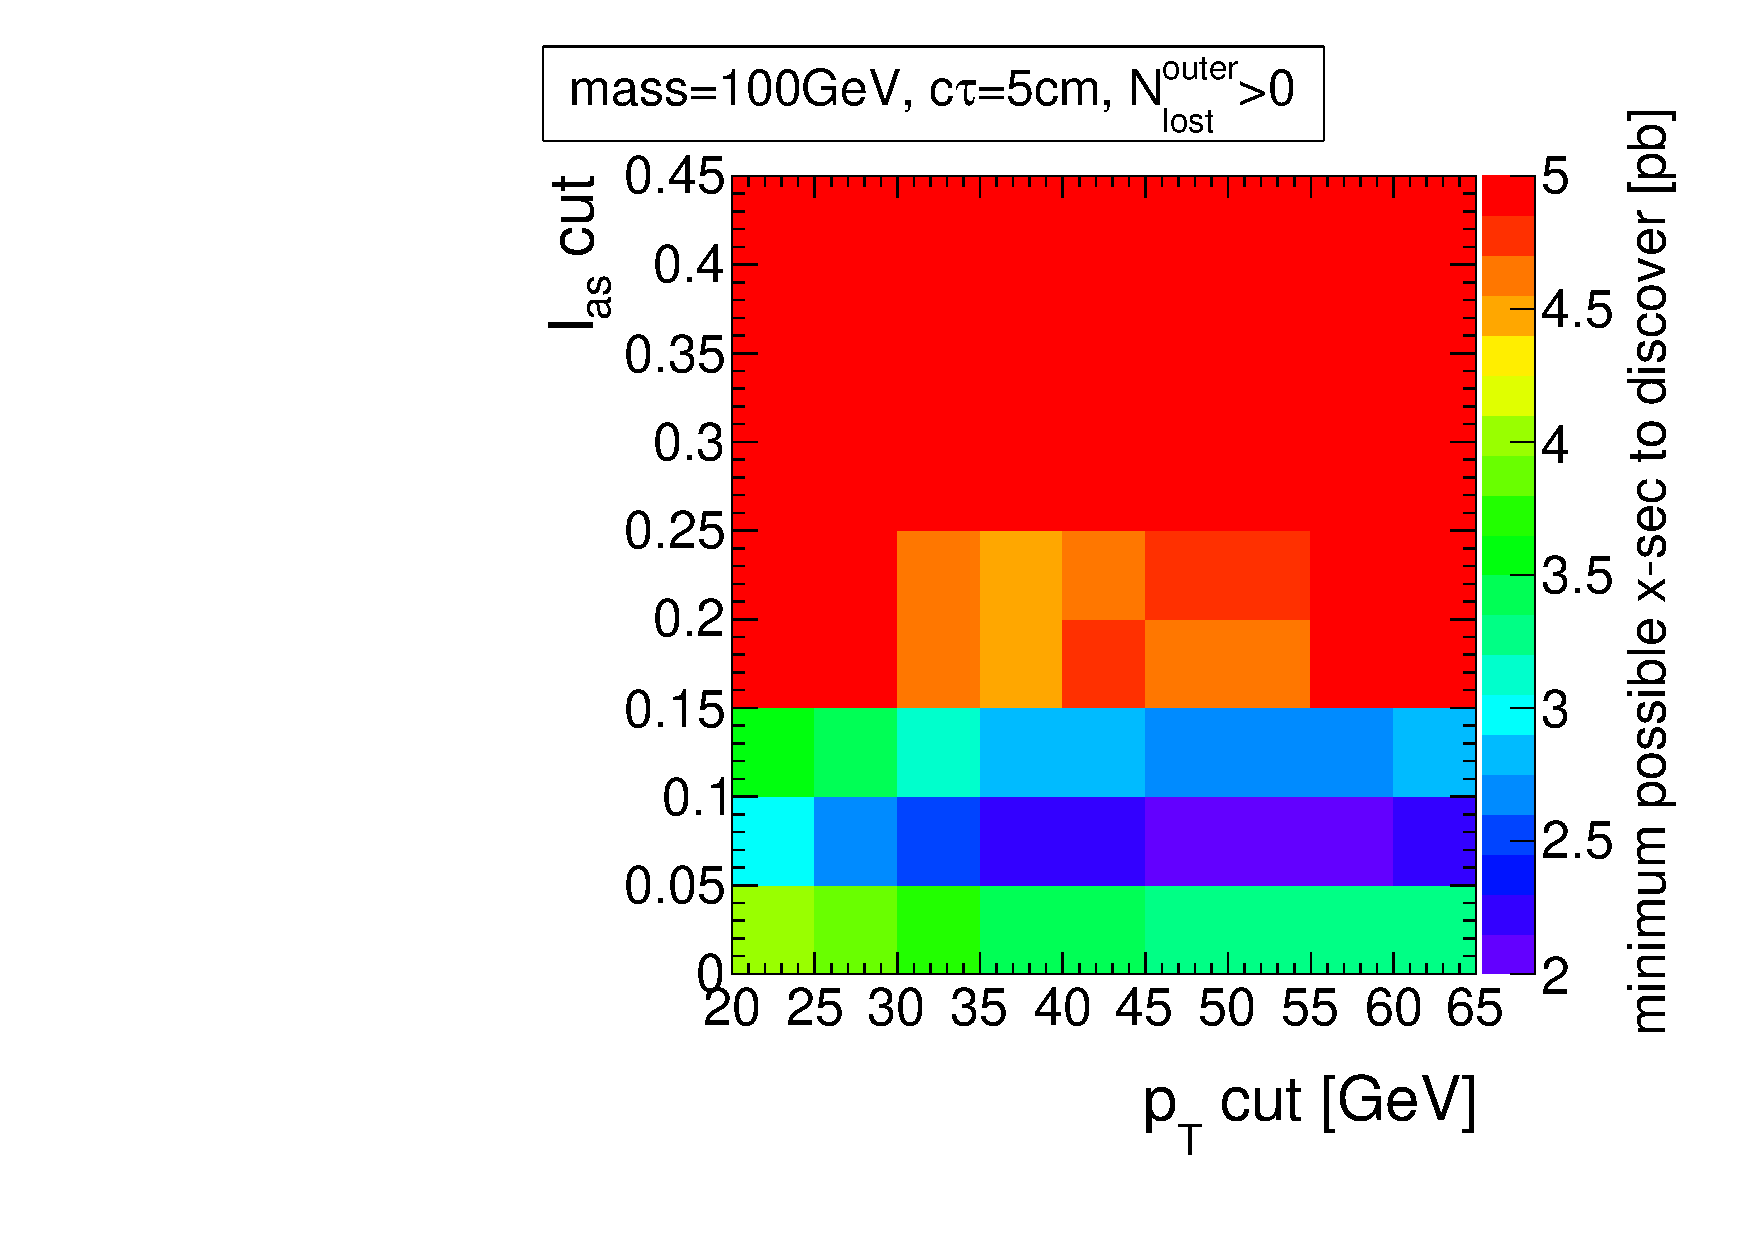
\includegraphics[width=0.33\textwidth]{figures/analysis/Optimisation/Madgraph_signal_mass_100_ctau_5cm_ECaloLe5_SOverDeltaBStatPlusSys_0.pdf} 
    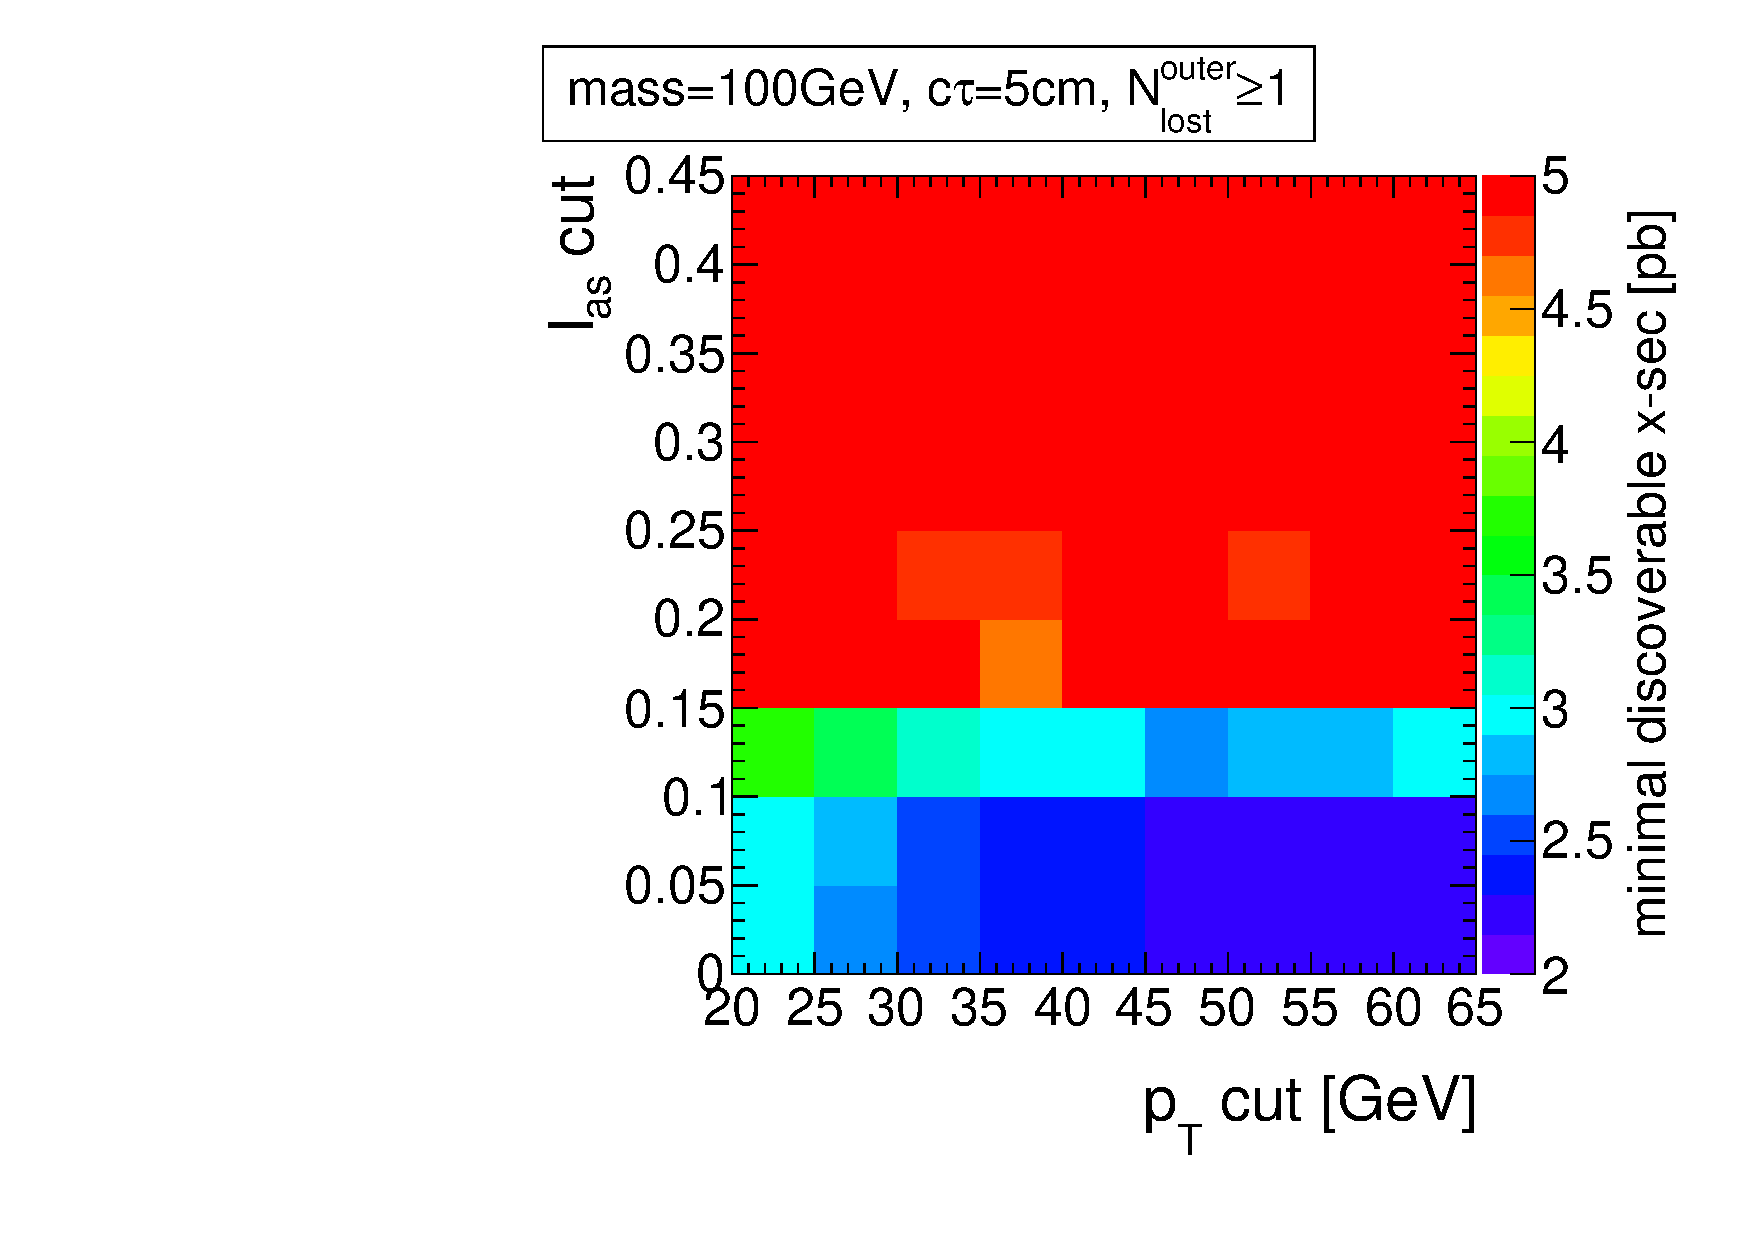
\includegraphics[width=0.33\textwidth]{figures/analysis/Optimisation/Madgraph_signal_mass_100_ctau_5cm_ECaloLe5_SOverDeltaBStatPlusSys_1.pdf} 
    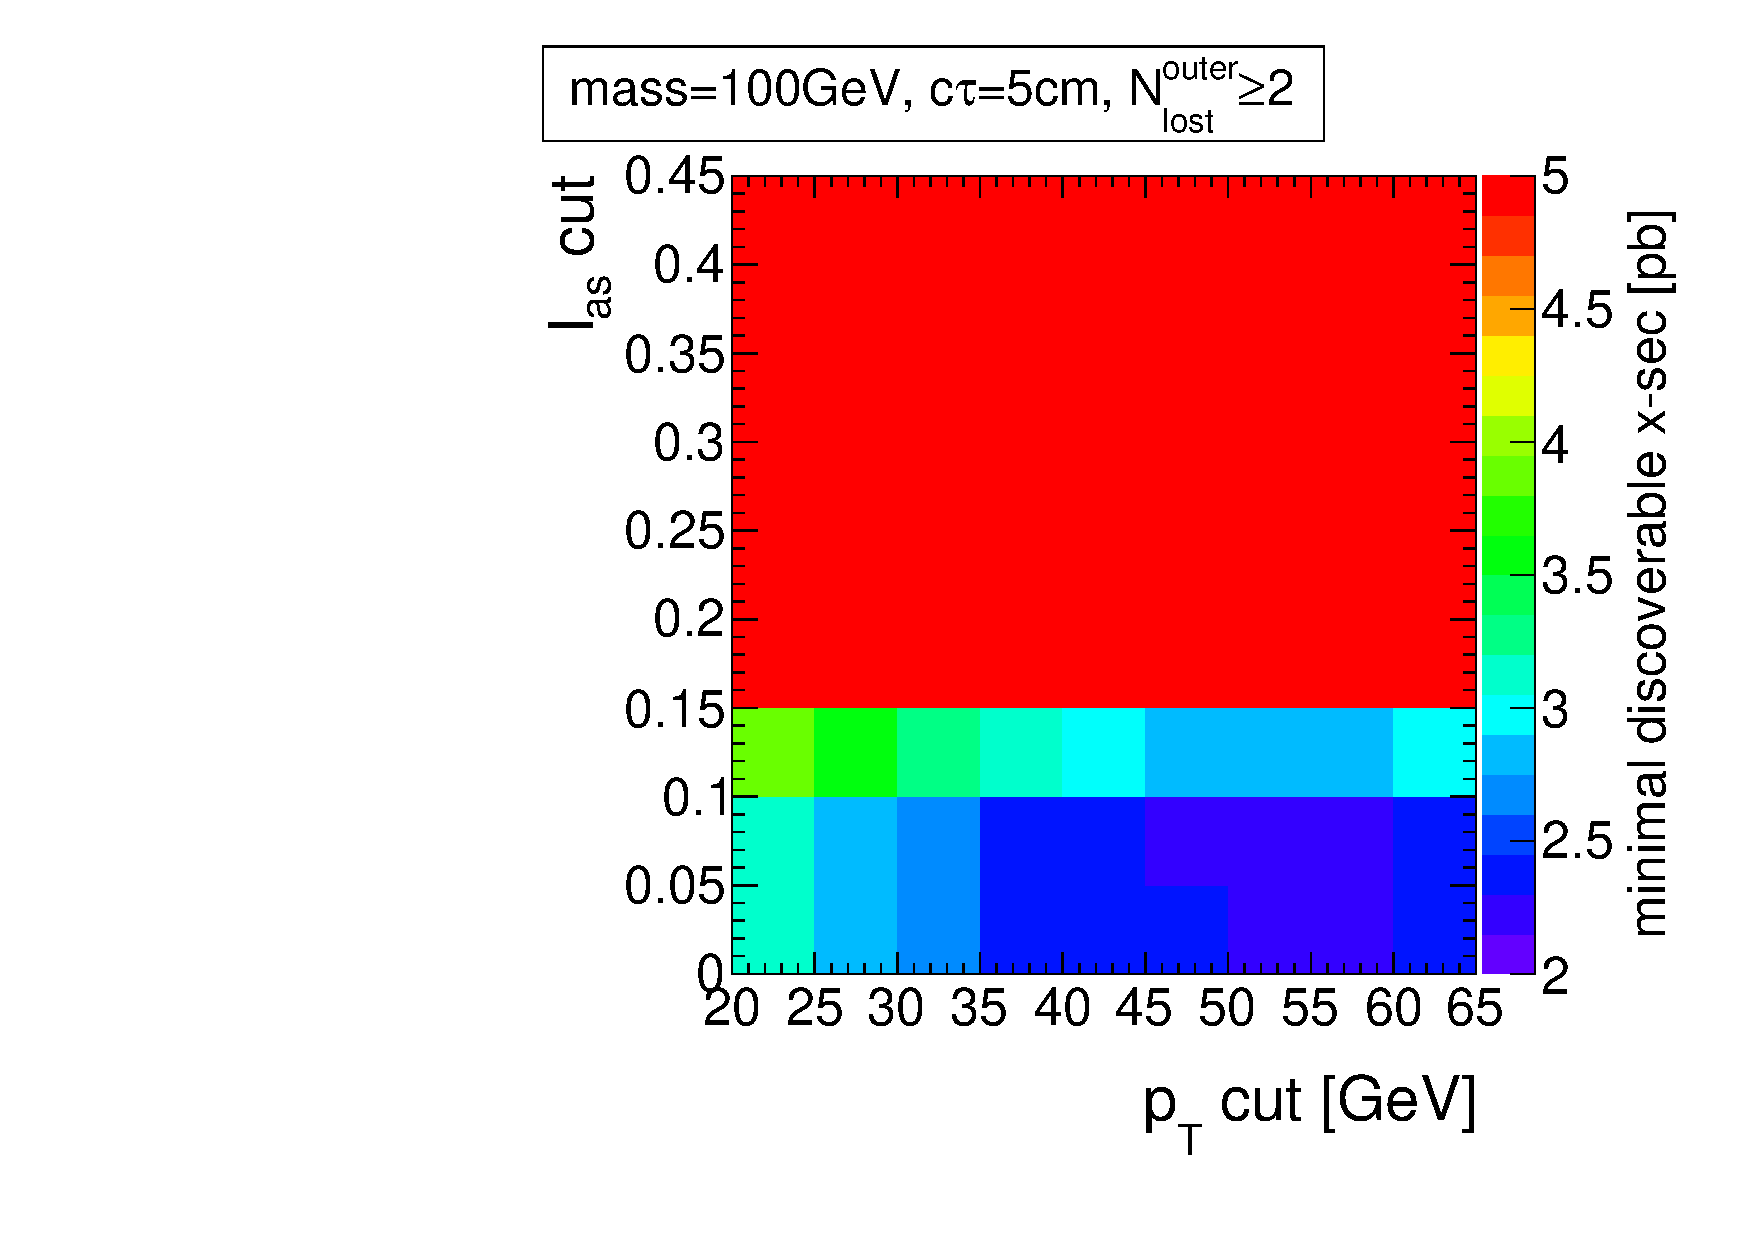
\includegraphics[width=0.33\textwidth]{figures/analysis/Optimisation/Madgraph_signal_mass_100_ctau_5cm_ECaloLe5_SOverDeltaBStatPlusSys_2.pdf} \\
    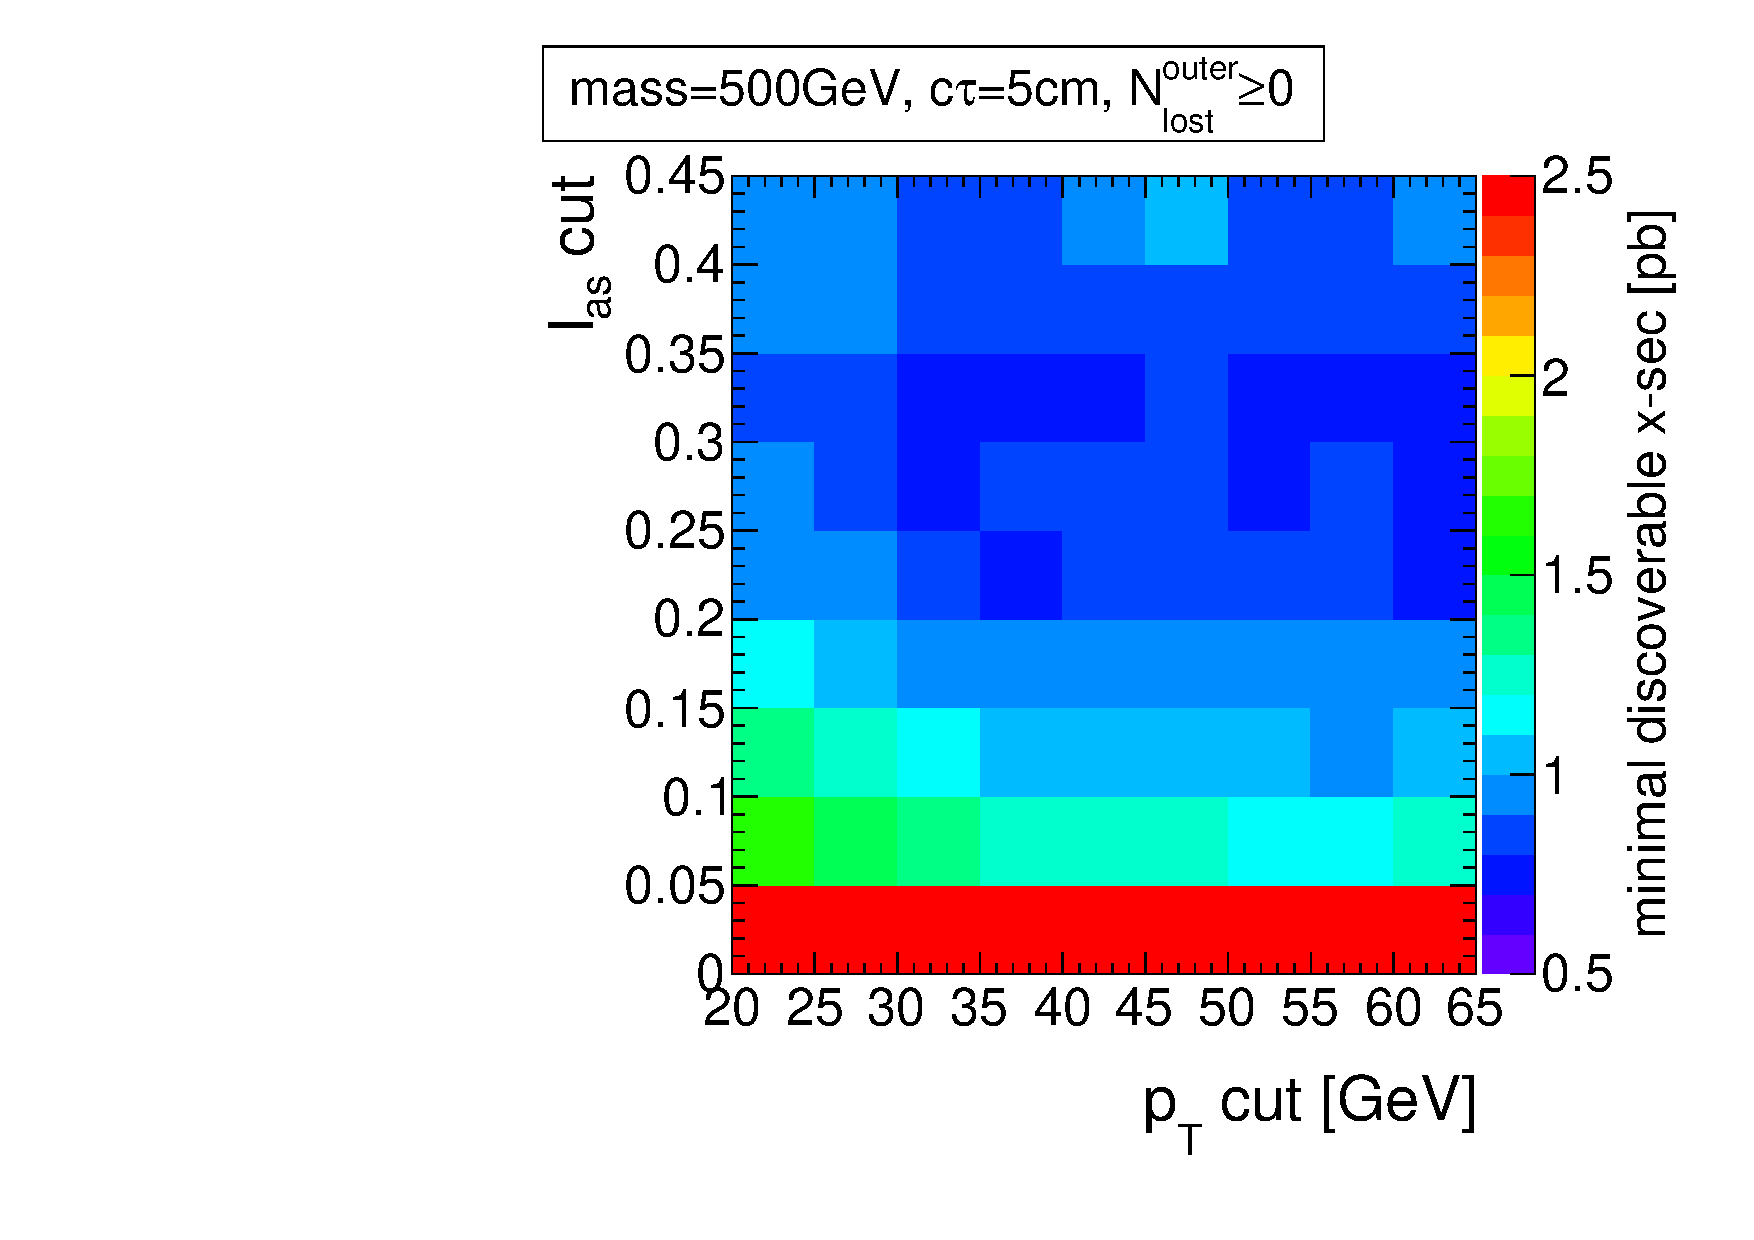
\includegraphics[width=0.33\textwidth]{figures/analysis/Optimisation/Madgraph_signal_mass_500_ctau_5cm_ECaloLe5_SOverDeltaBStatPlusSys_0.pdf} 
    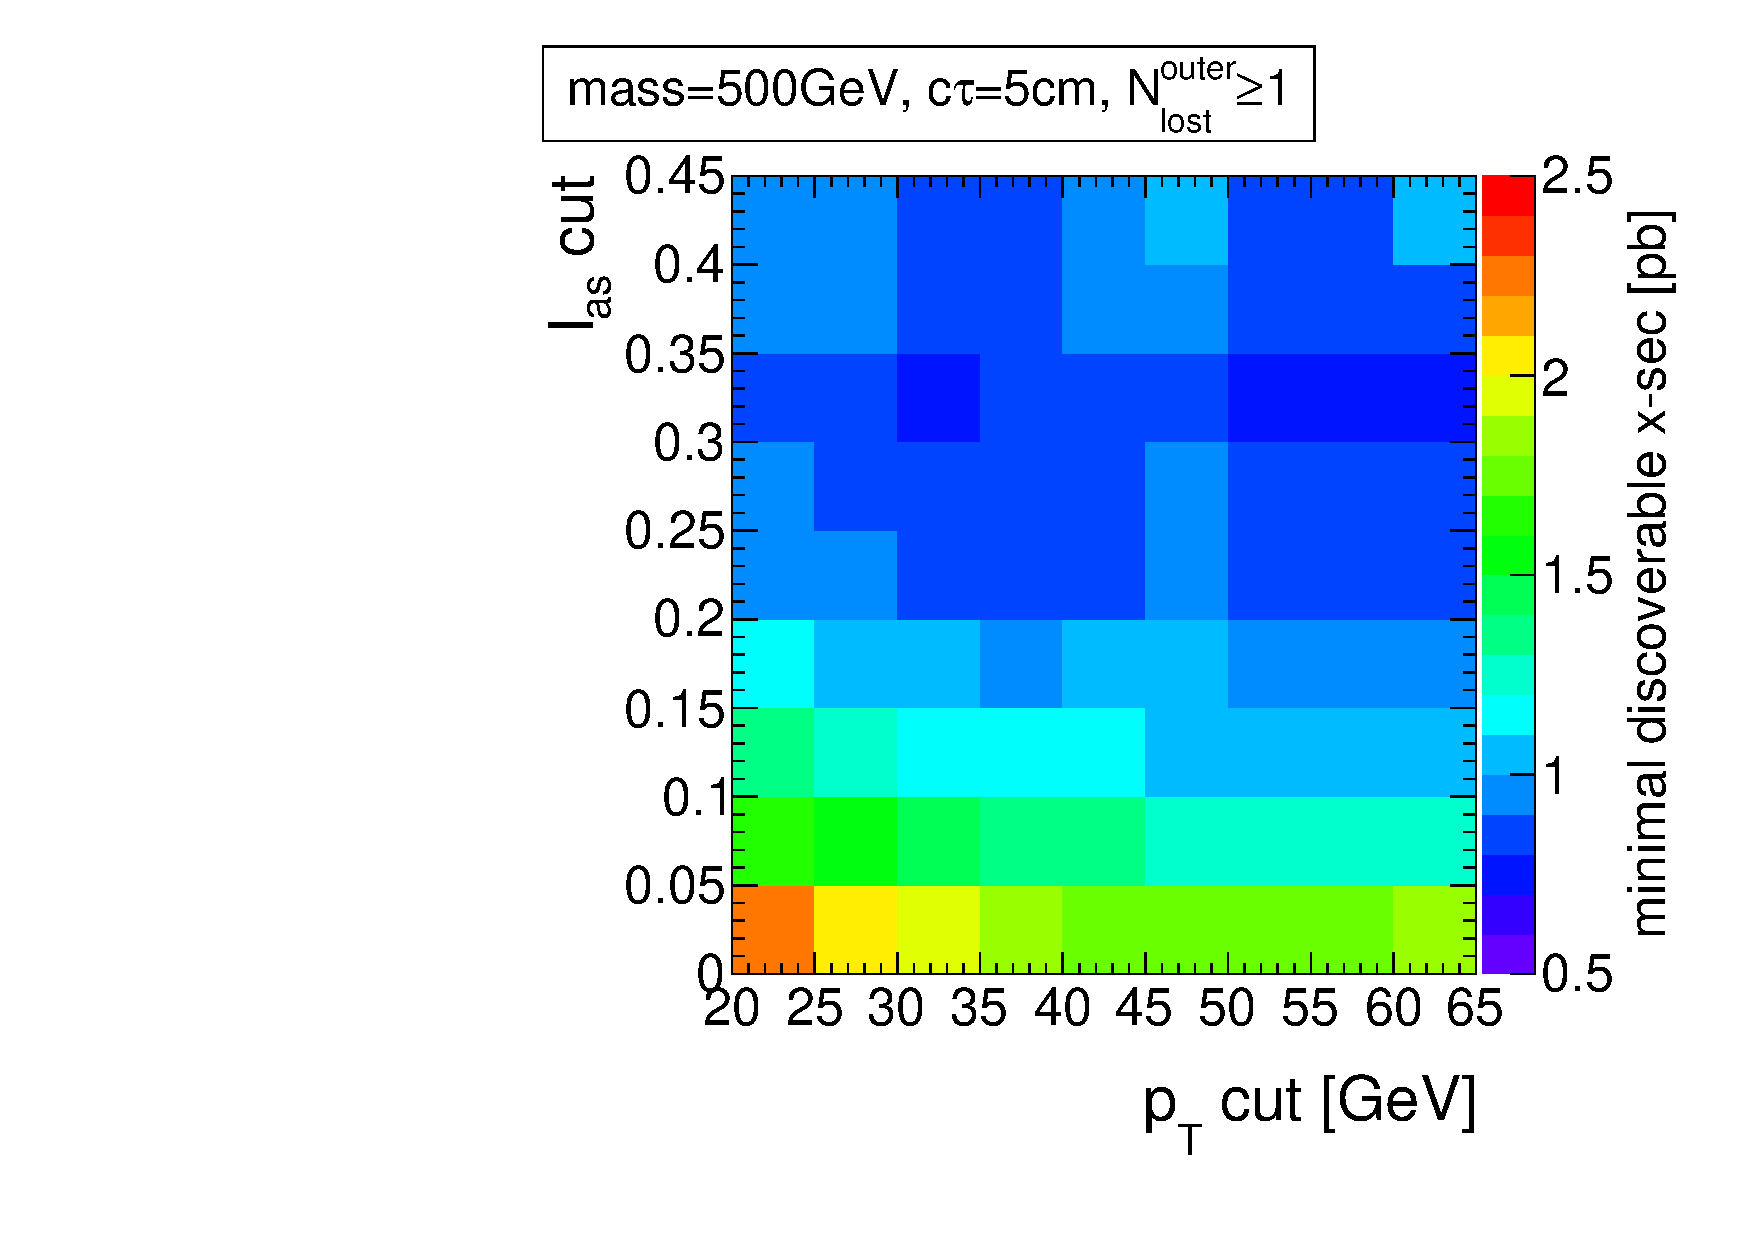
\includegraphics[width=0.33\textwidth]{figures/analysis/Optimisation/Madgraph_signal_mass_500_ctau_5cm_ECaloLe5_SOverDeltaBStatPlusSys_1.pdf}
    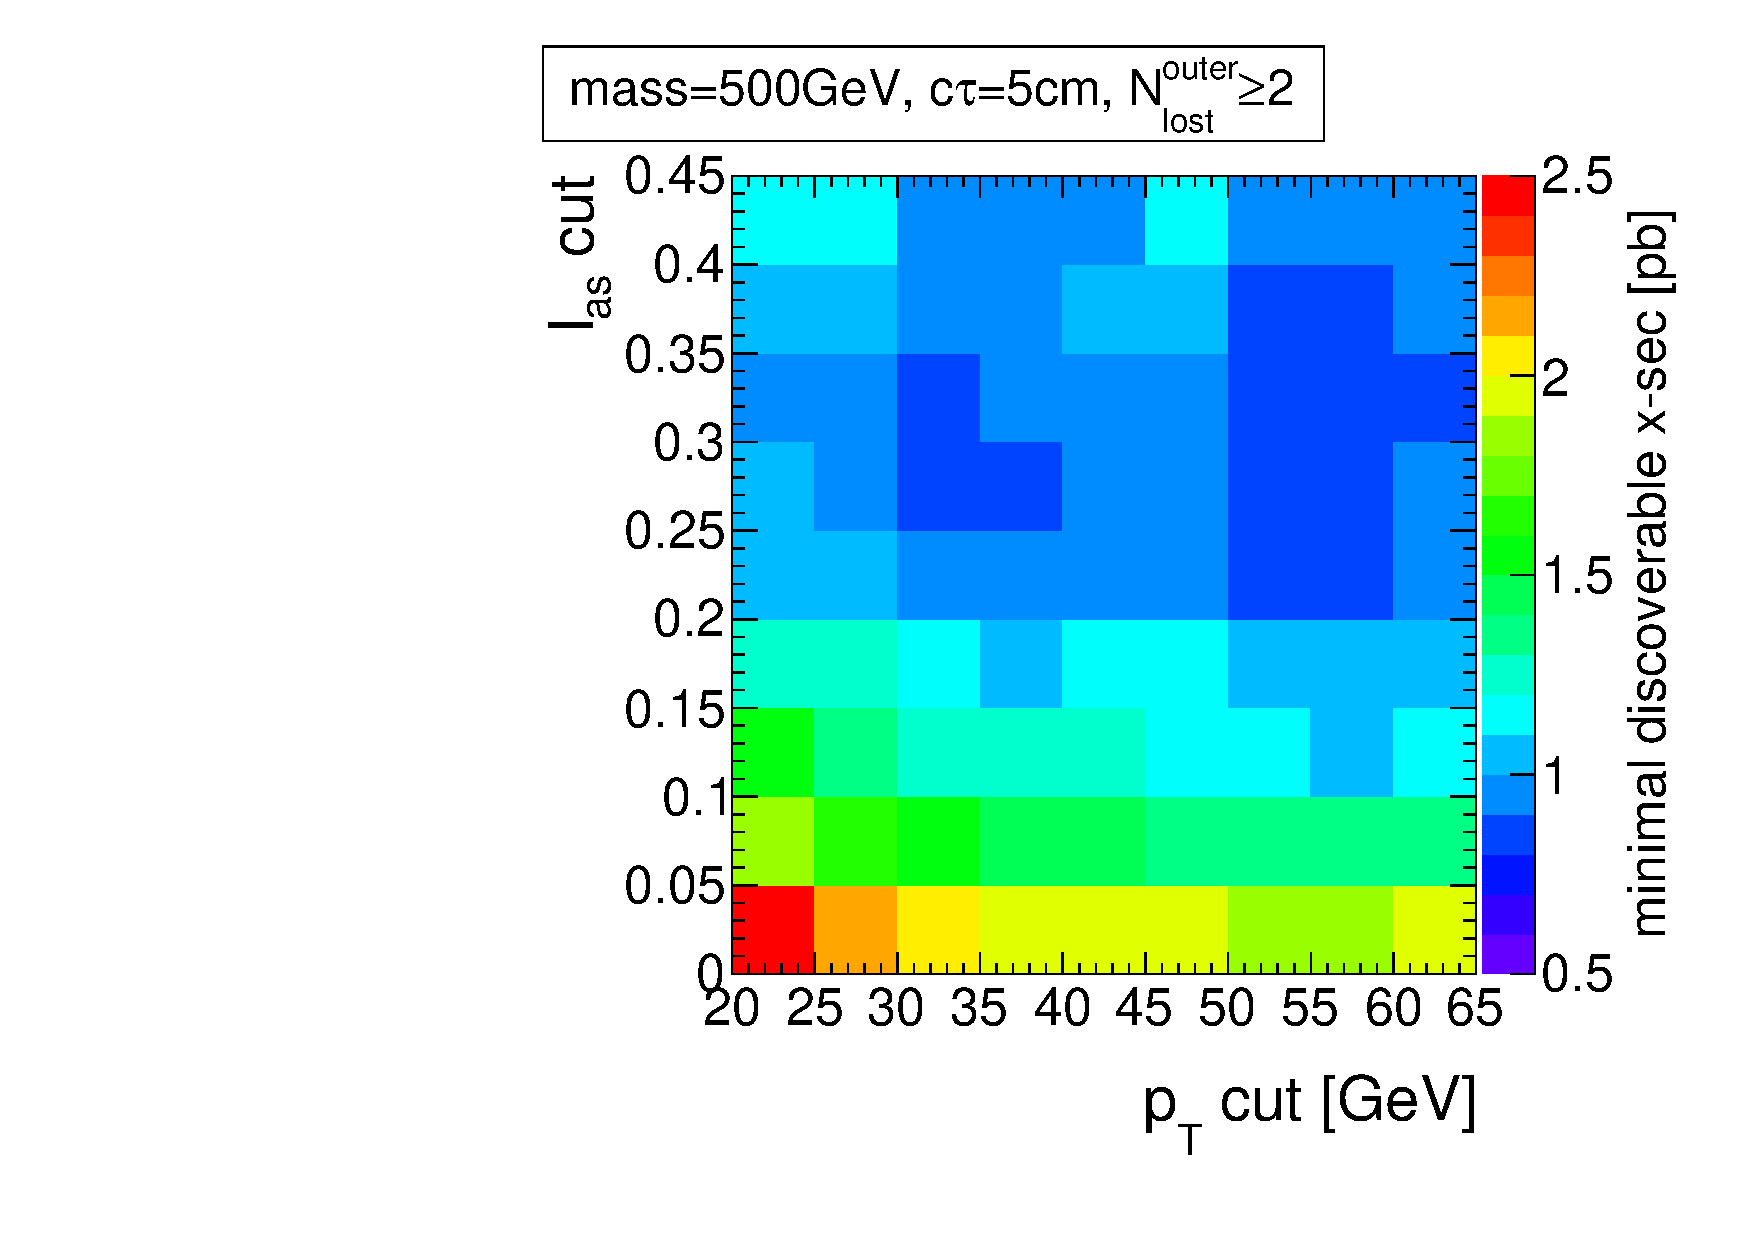
\includegraphics[width=0.33\textwidth]{figures/analysis/Optimisation/Madgraph_signal_mass_500_ctau_5cm_ECaloLe5_SOverDeltaBStatPlusSys_2.pdf} 
  \end{tabular}
  \caption{Minimum possible cross section that can be discovered with 5$\sigma$ significance in the $\ias - \pt$ plane for two different signal models with a chargino lifetime of 5\cm and a mass of 100\gev (top) and 500\gev (bottom).
           The requirement on the number of missing outer hits is varied between $\nlostouter>0$ (left), $\nlostouter>1$ (middle) and $\nlostouter>2$ (right). 
           A difference in the sensitivity can be spotted when looking at the lowest value of the minimal discoverable cross section that occurs.
           No sizable discrimination improvement is visible for a tighter selection in \nlostouter.}
  \label{fig:optimisationNLostOuter}
\end{figure} 
This is caused by the fact, that the main background, the fake background, also shows missing outer hits.
A comparison between the number of missing outer hits for the fake background and two signal models is shown in Fig.~\ref{fig:NLostOuterFakeSignal}.
\begin{figure}[!h]
  \centering 
  \begin{tabular}{c}
    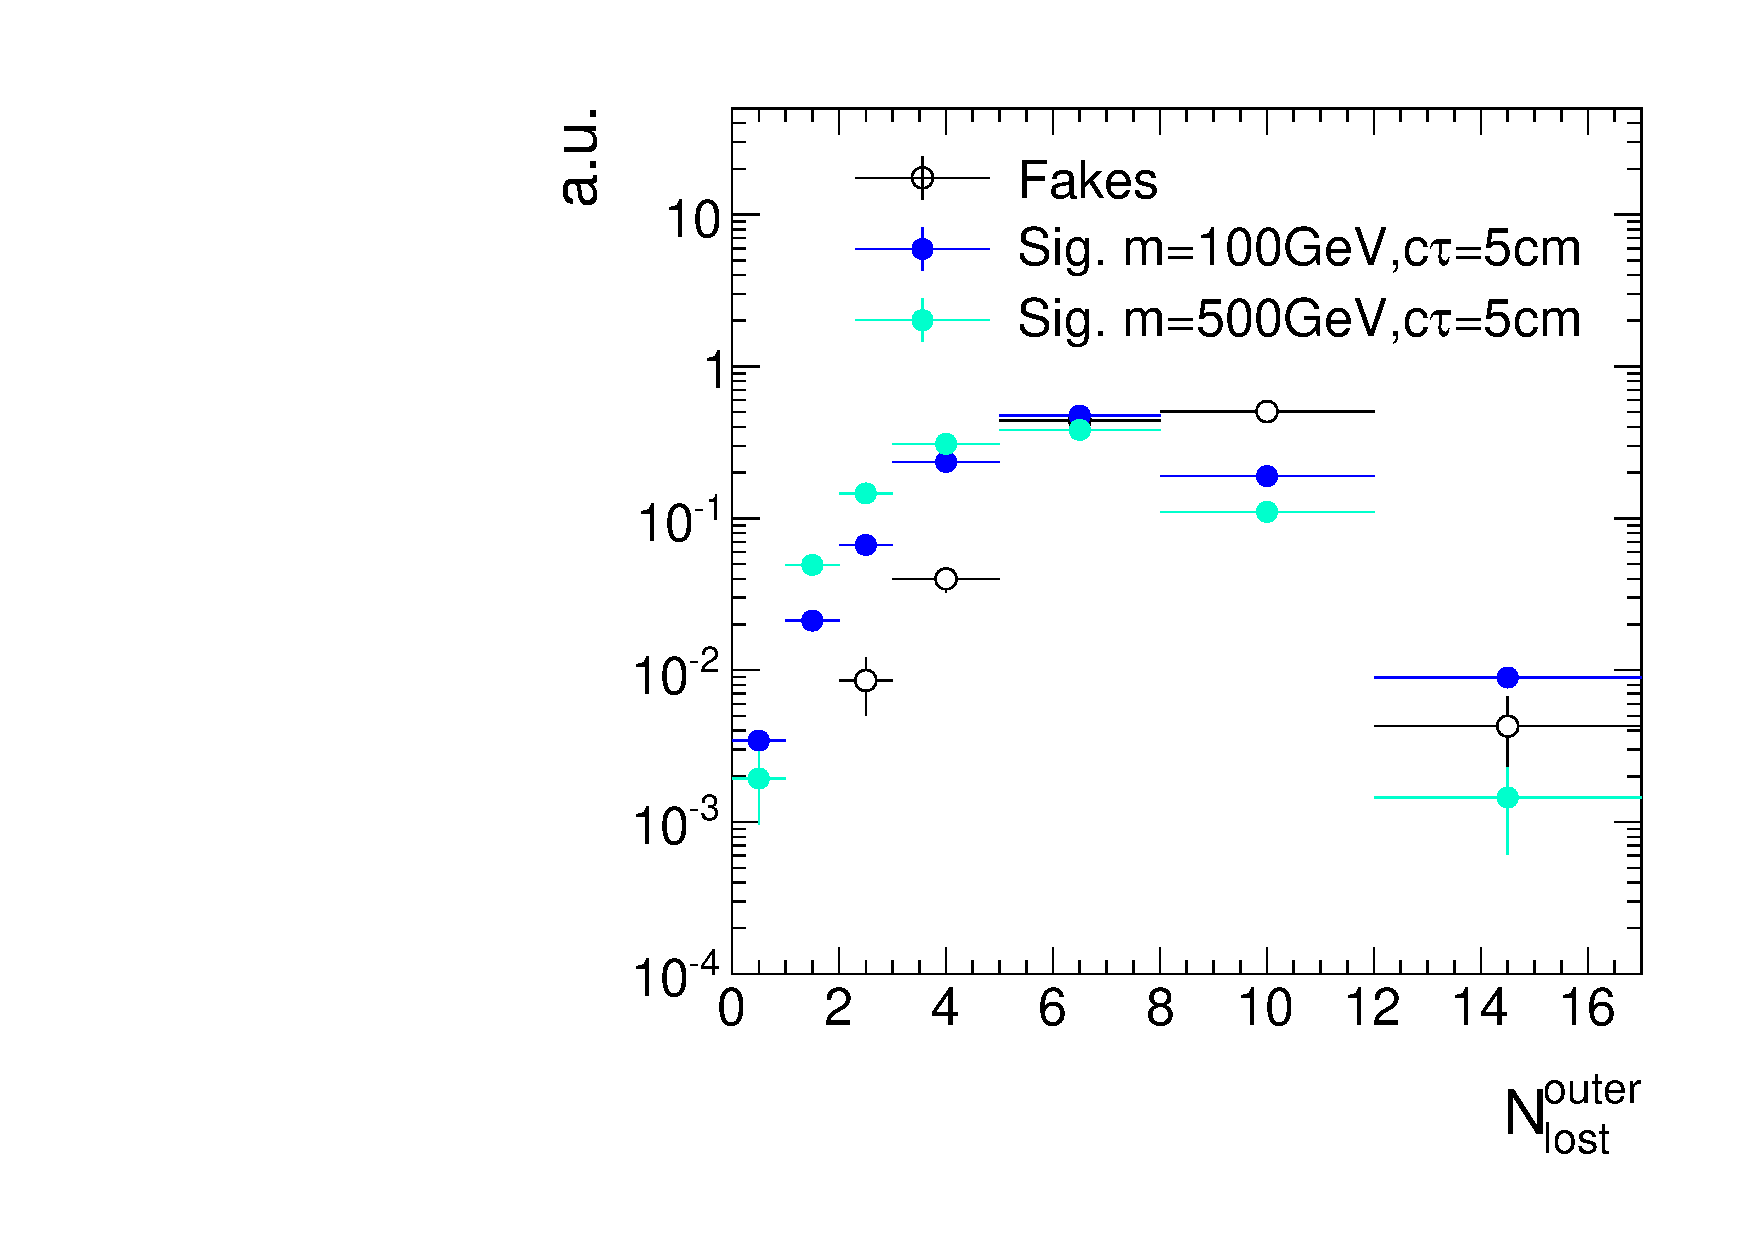
\includegraphics[width=0.39\textwidth]{figures/analysis/Optimisation/NLostOuterForFakes_chiTracksfullSelectionNoQCDCutsNoTrigger.pdf} 
  \end{tabular}
  \caption{Normalised distribution of the number of missing outer hits for fake tracks and two different signal models. }
  \label{fig:NLostOuterFakeSignal}
\end{figure} 

\FloatBarrier
\section{Underlying distributions for the qualitative search sensitivity optimisation}
\label{app:OptimisationApp}

\begin{figure}[!h]
  \centering 
  \begin{tabular}{c}
    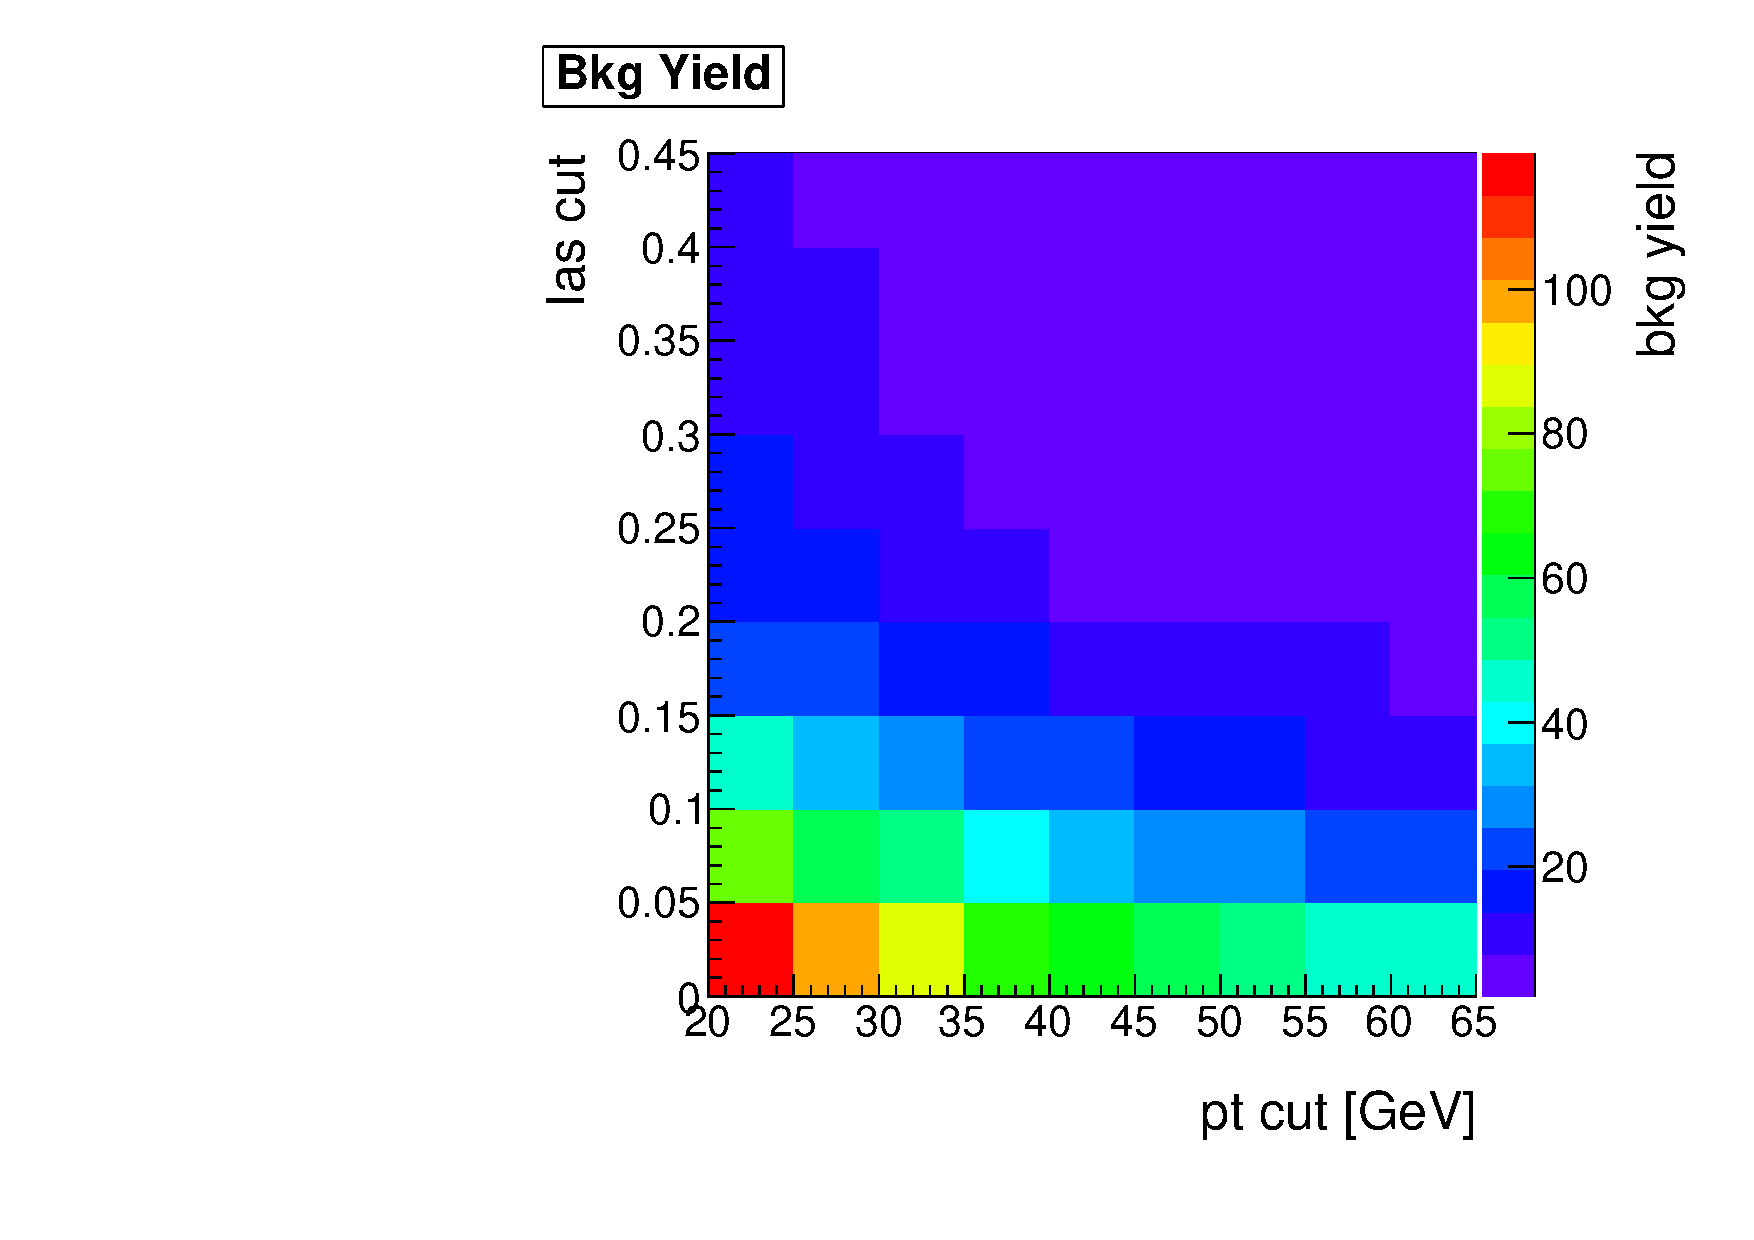
\includegraphics[width=0.33\textwidth]{figures/analysis/Optimisation/BkgYield_ECaloLe5.pdf} 
    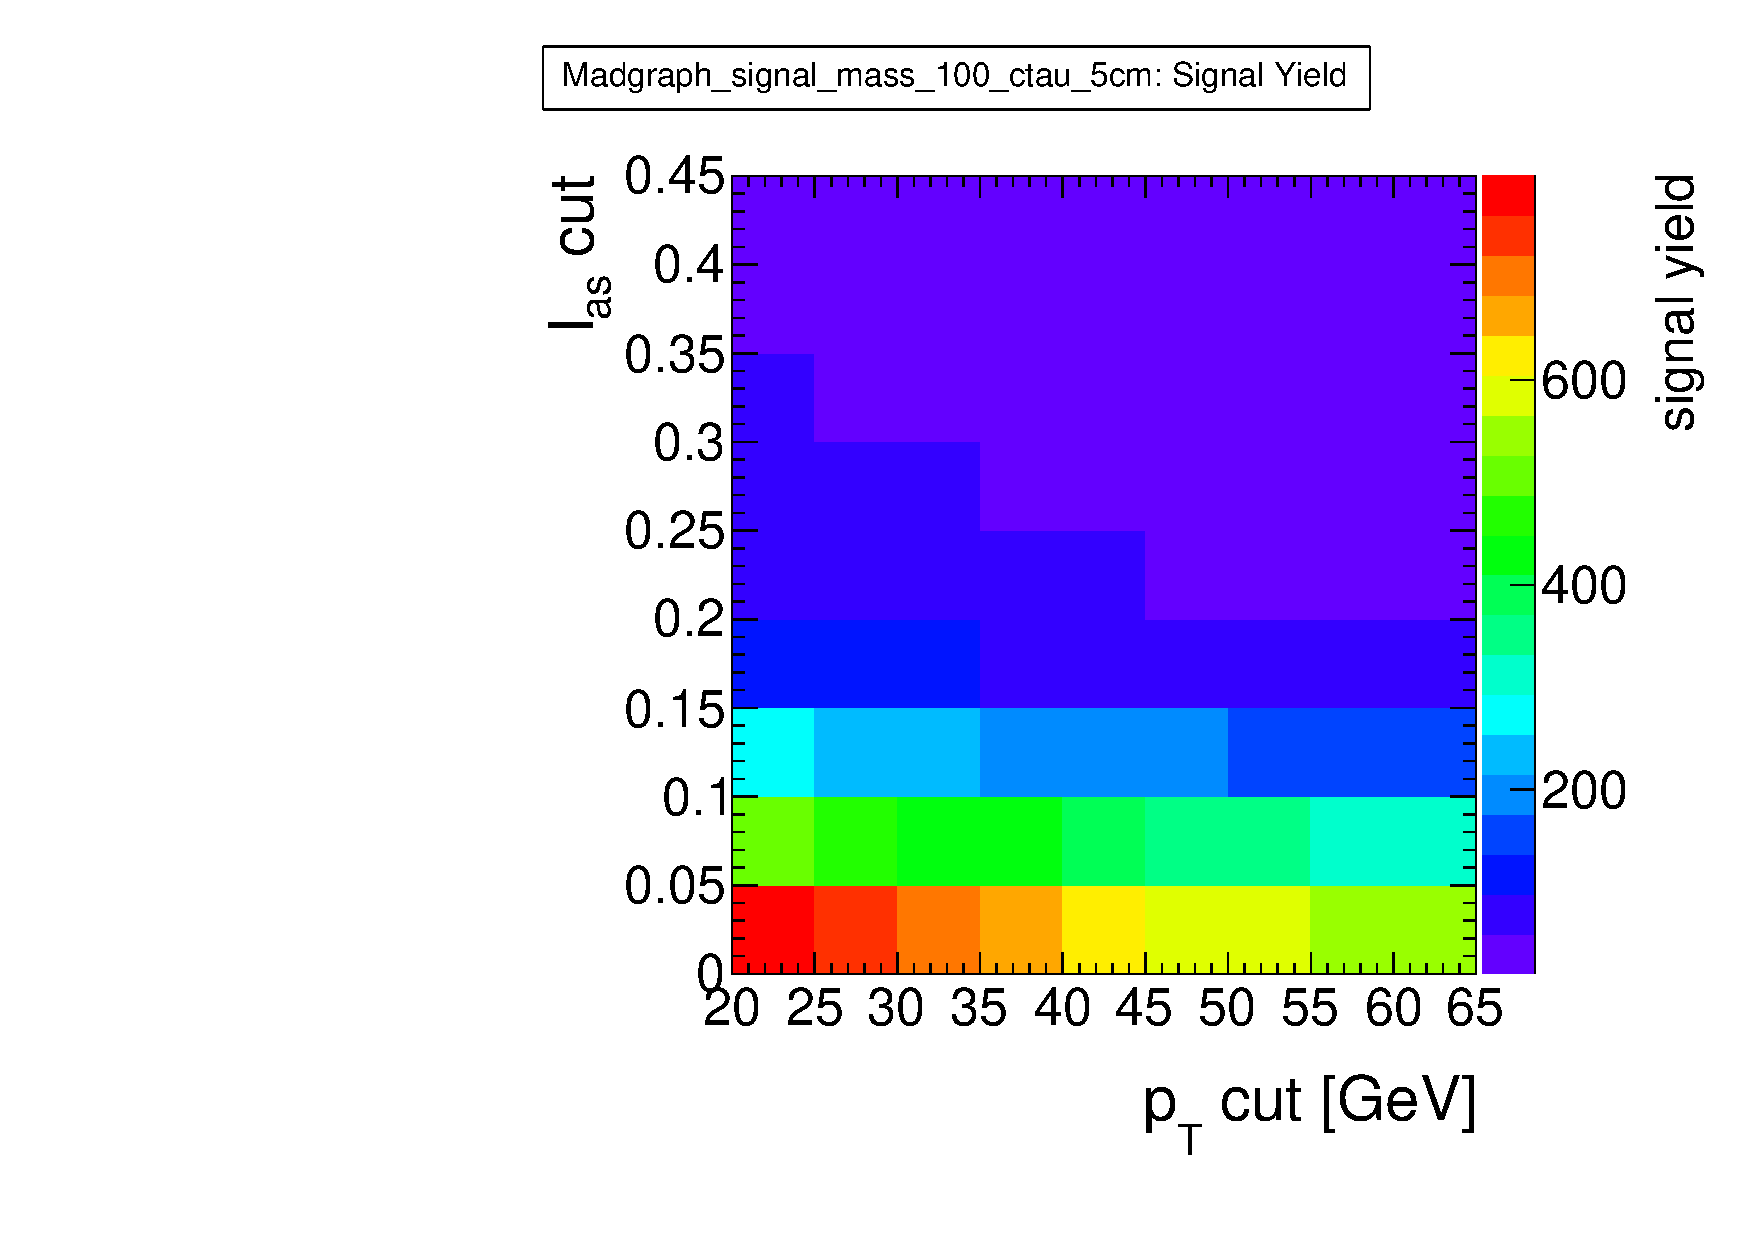
\includegraphics[width=0.33\textwidth]{figures/analysis/Optimisation/Madgraph_signal_mass_100_ctau_5cm_ECaloLe5_SignalYield.pdf}
    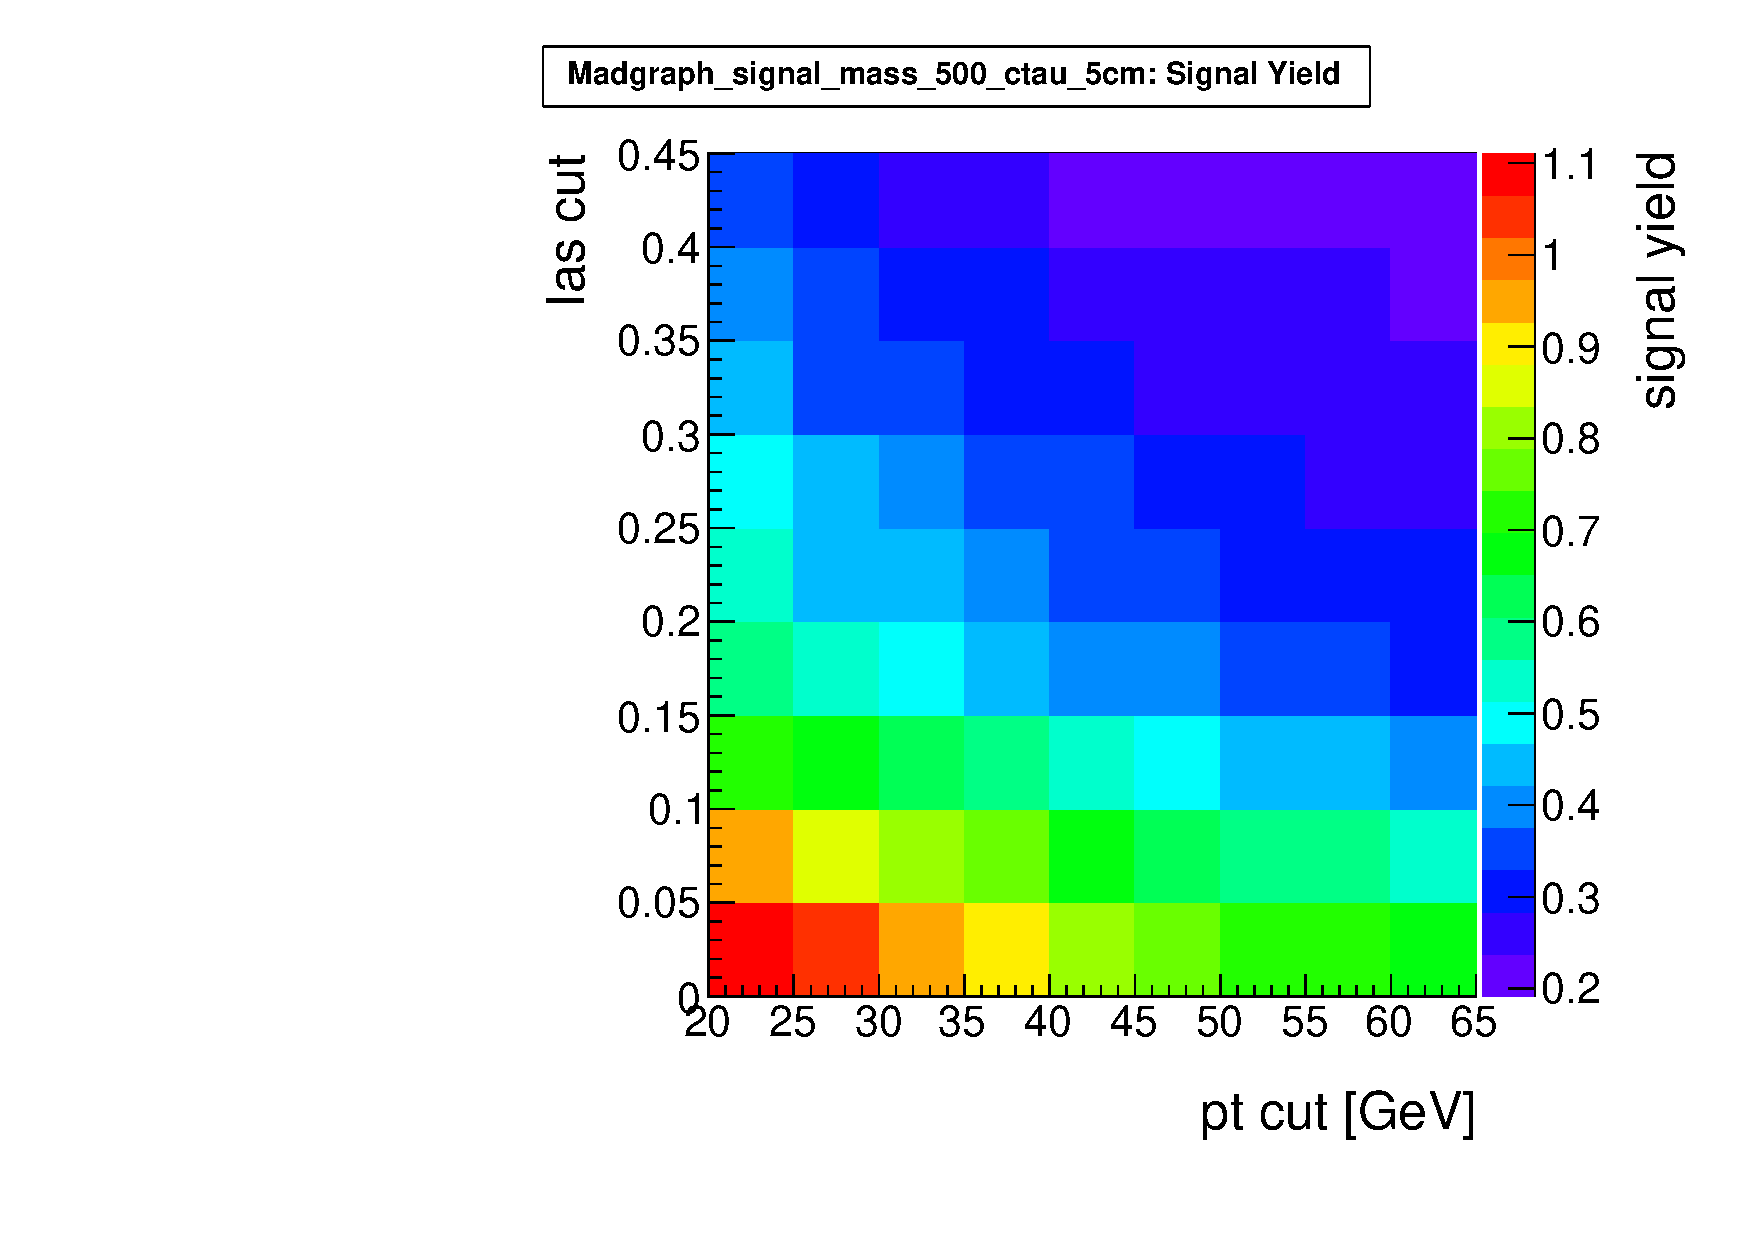
\includegraphics[width=0.33\textwidth]{figures/analysis/Optimisation/Madgraph_signal_mass_500_ctau_5cm_ECaloLe5_SignalYield.pdf}\\
    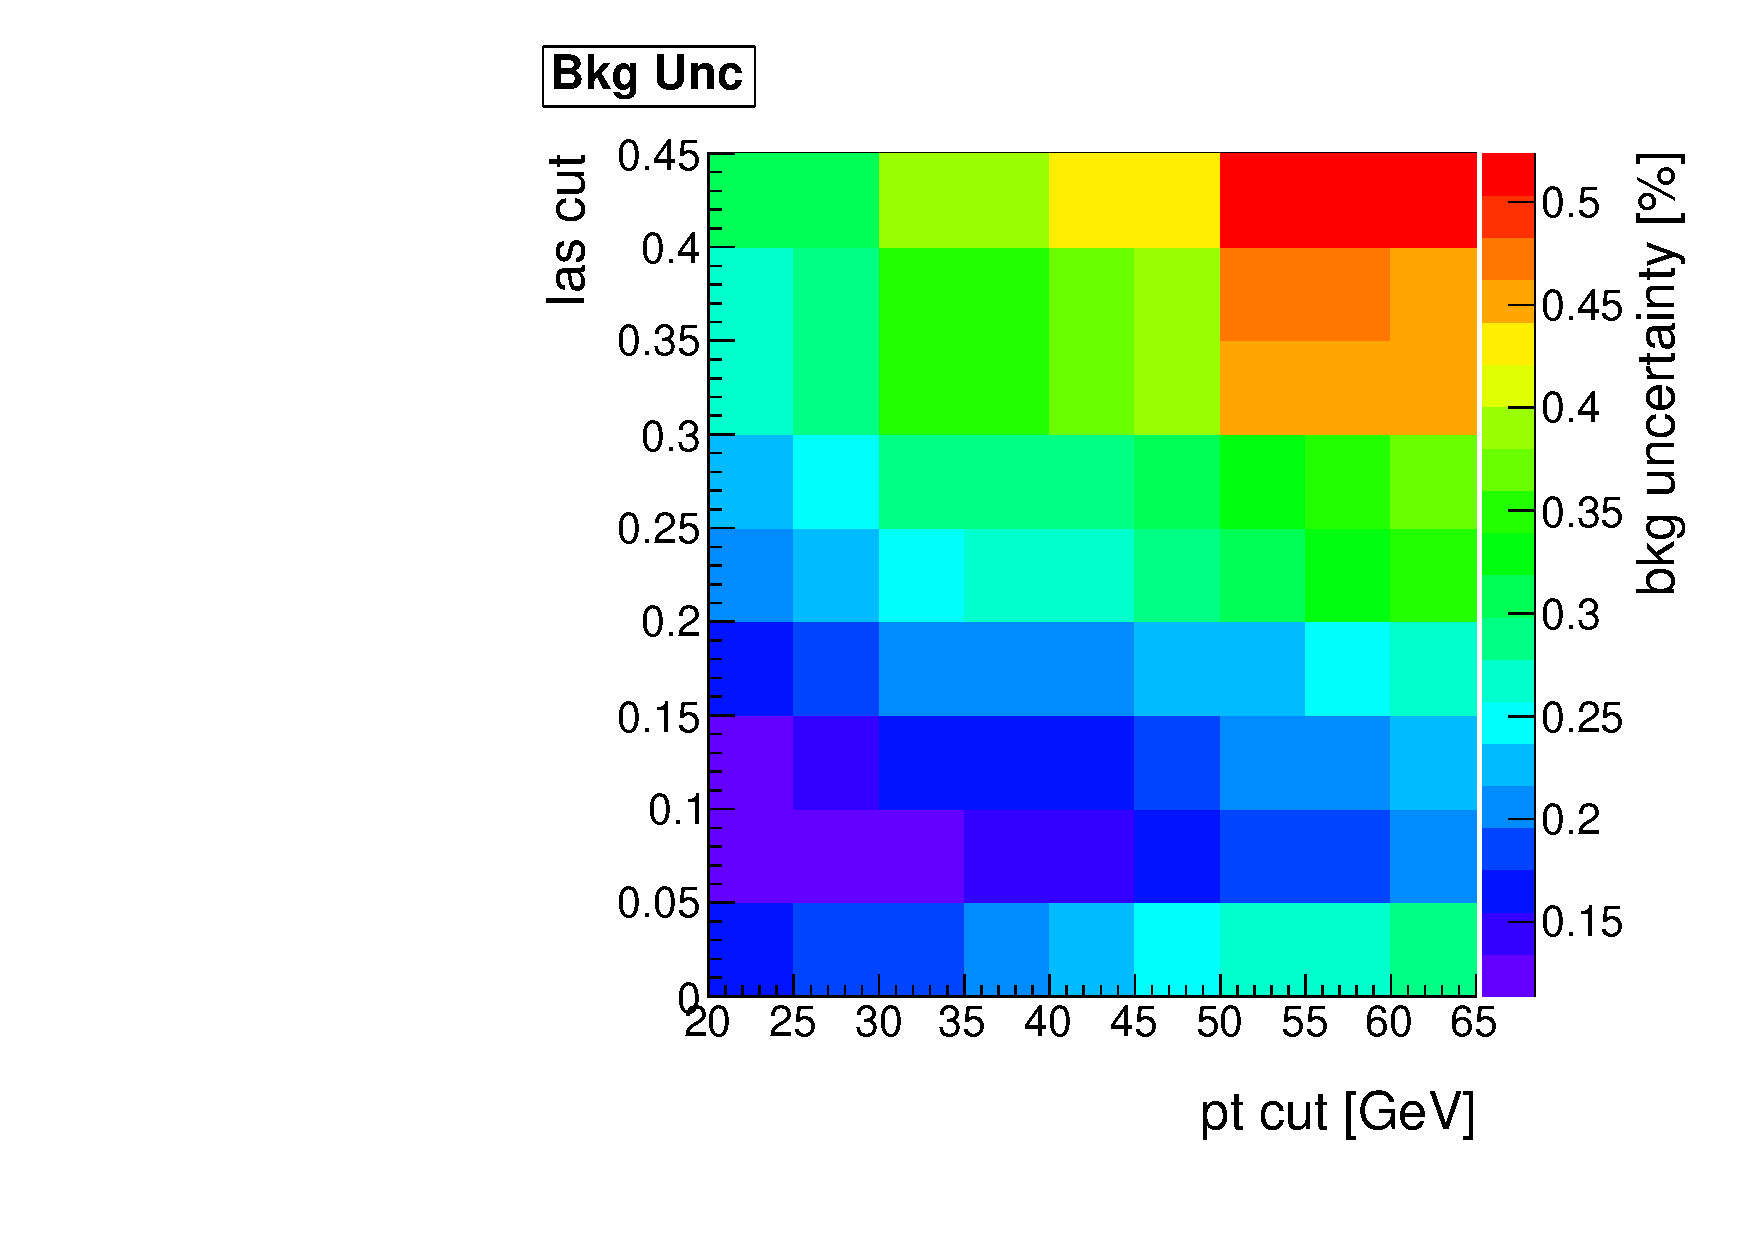
\includegraphics[width=0.33\textwidth]{figures/analysis/Optimisation/BkgUncertainty_ECaloLe5.pdf} 
    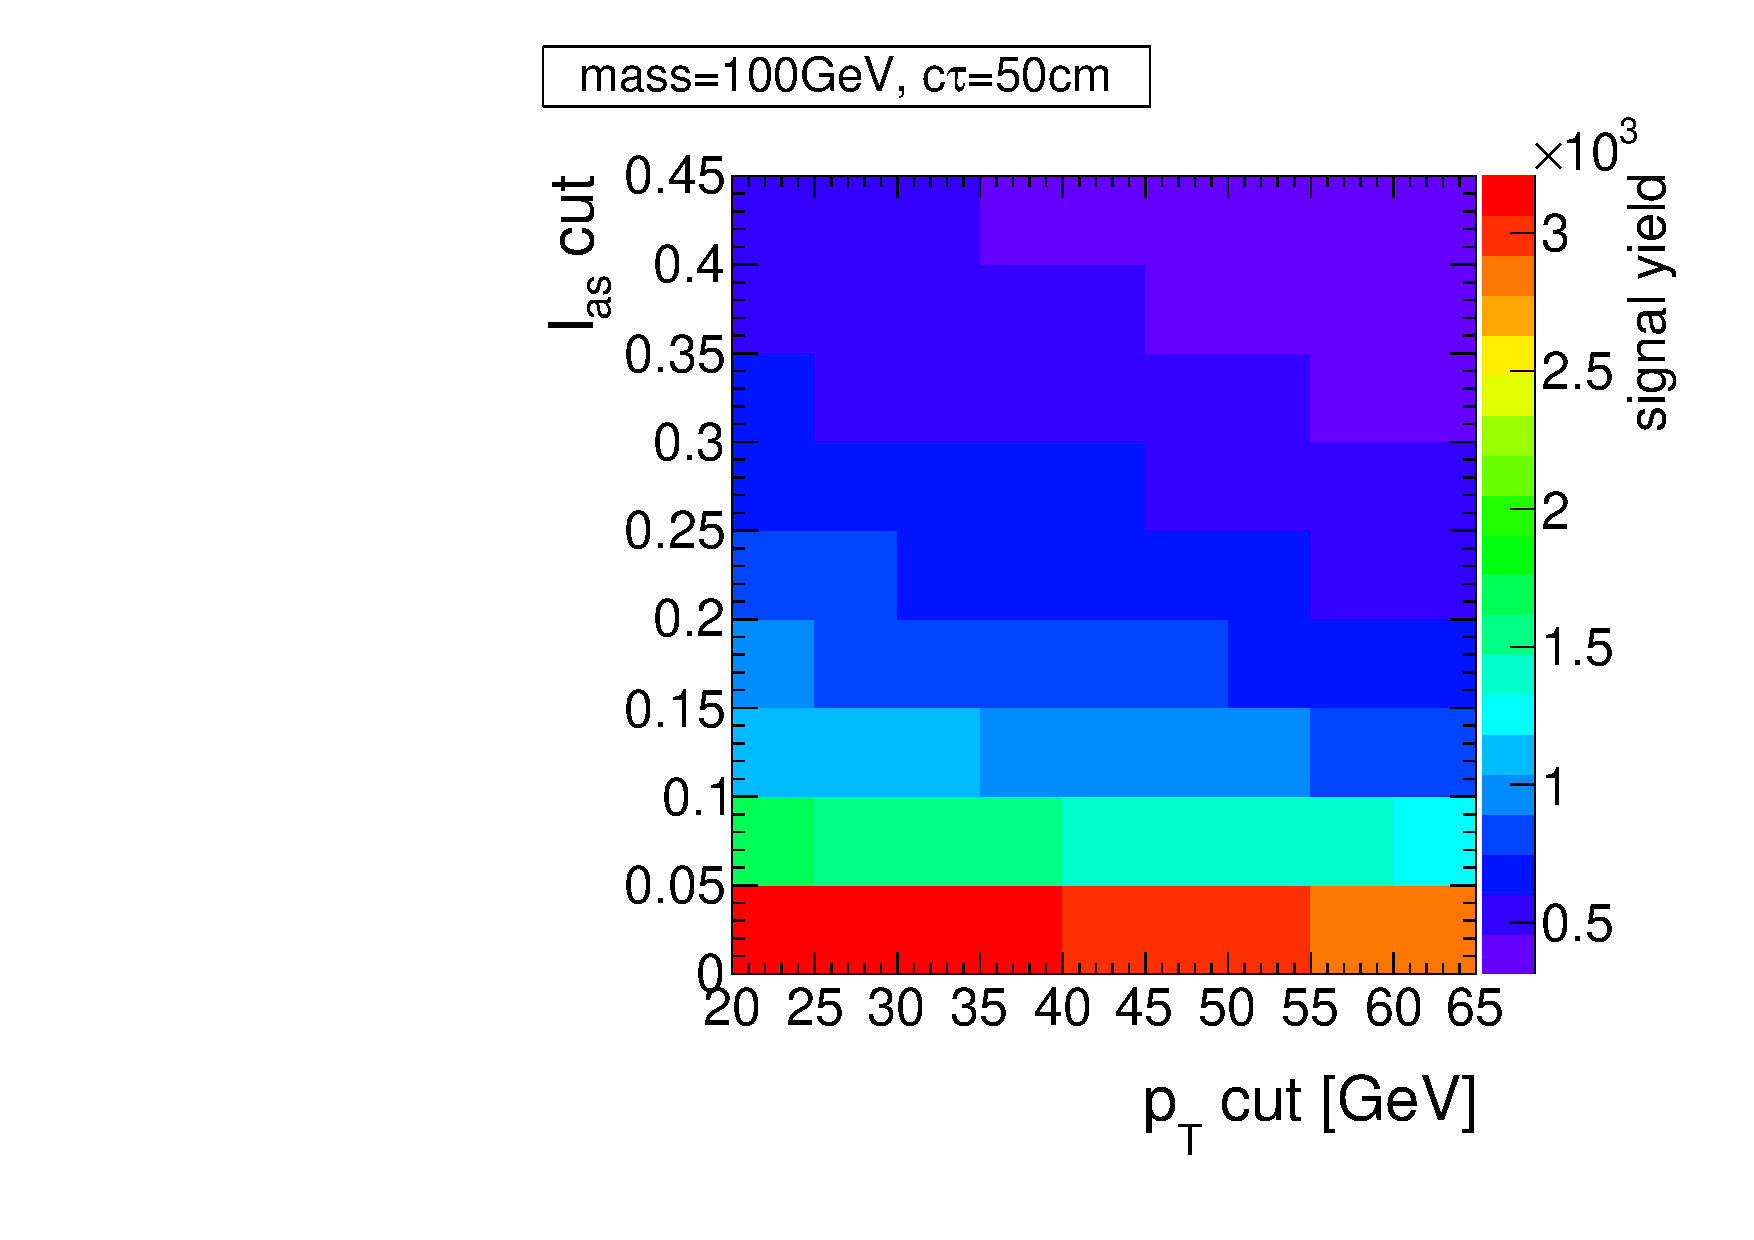
\includegraphics[width=0.33\textwidth]{figures/analysis/Optimisation/Madgraph_signal_mass_100_ctau_50cm_ECaloLe5_SignalYield.pdf}
    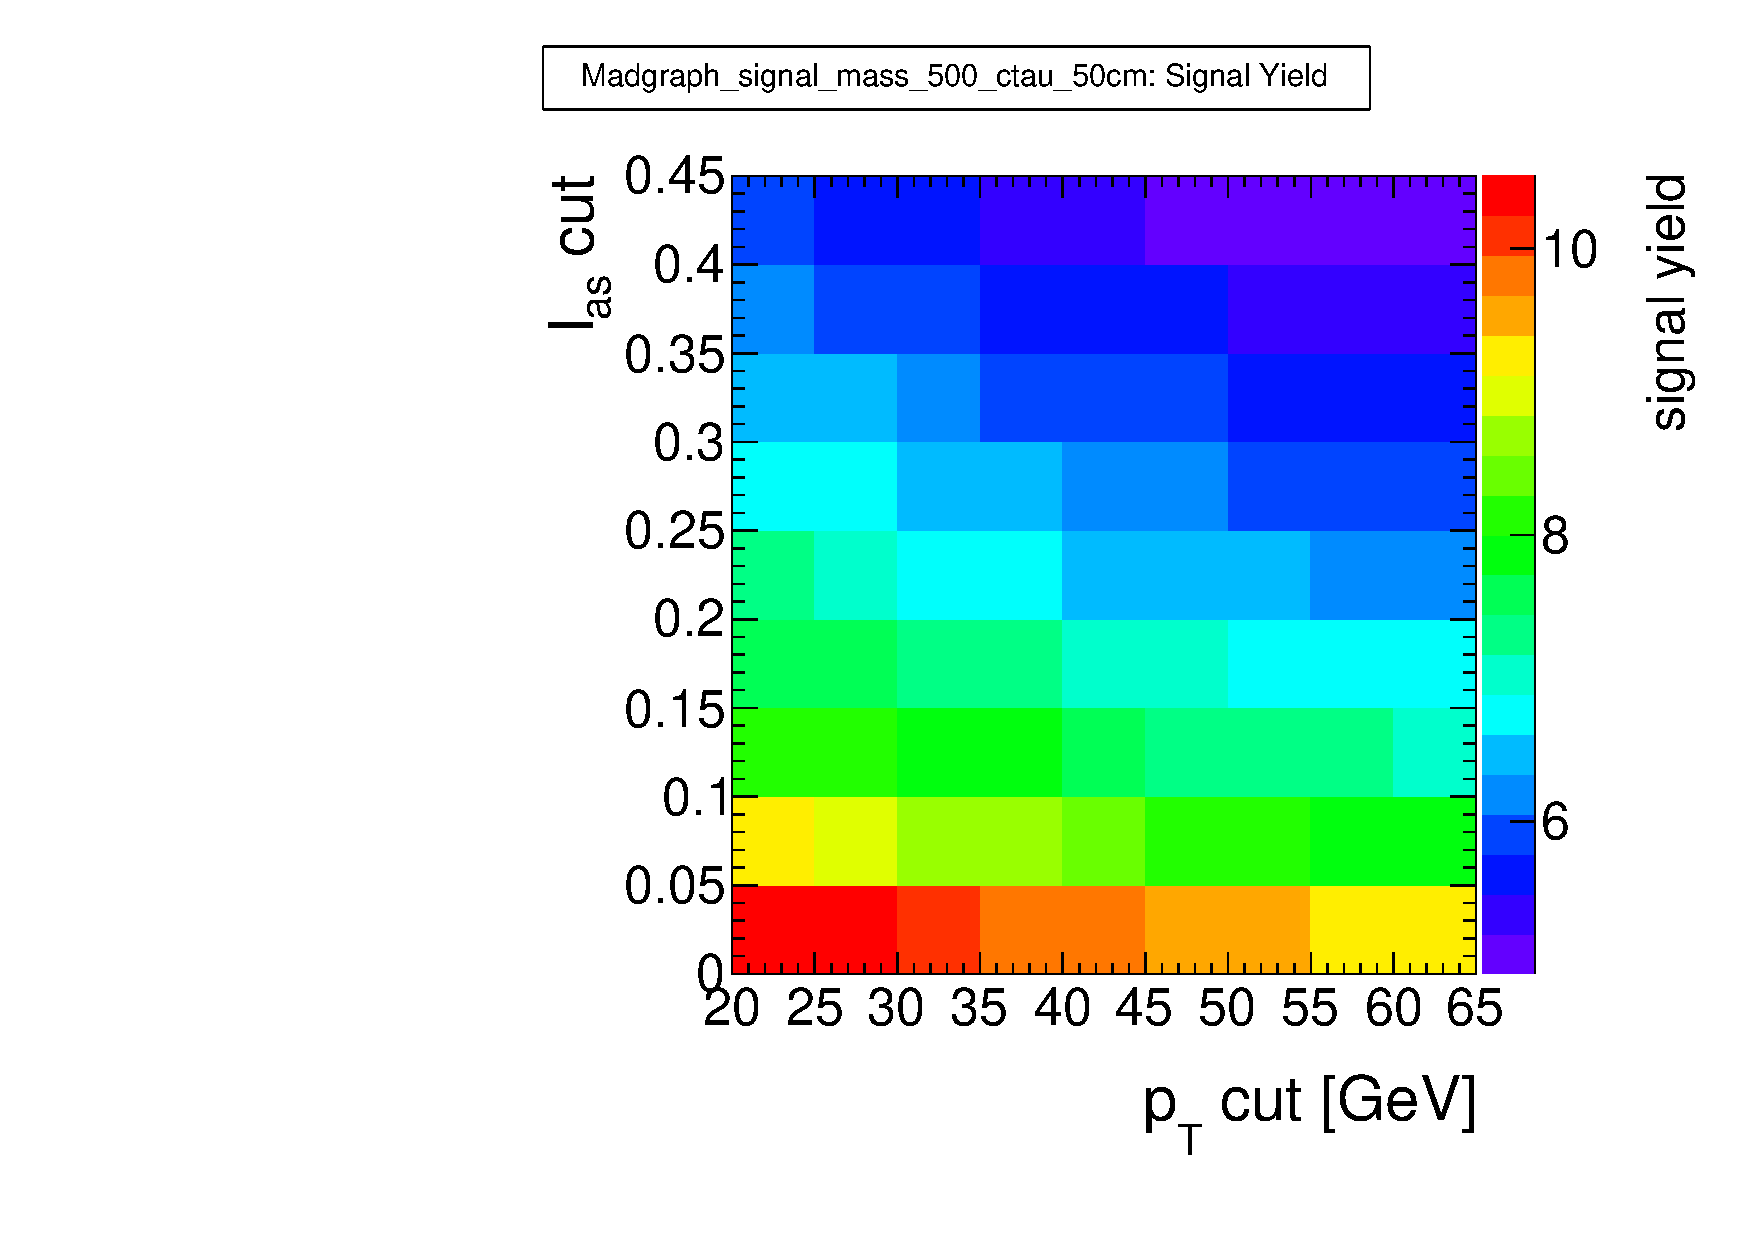
\includegraphics[width=0.33\textwidth]{figures/analysis/Optimisation/Madgraph_signal_mass_500_ctau_50cm_ECaloLe5_SignalYield.pdf}
  \end{tabular}
  \caption{Background yield, background uncertainty and signal yield for different \pt and \ias selection requirements and four different signal models.}
  \label{fig:optimisationApp}
\end{figure} 


%%%%%%%%%%%%%%%%%%%%%%%%%%%%%%%%%%%%%%%%%%%%%%%%%%%%%%%%%%%%%%%%%%%%%%%%%%%%%%%%%%%%%%%%%%%%%%%%%%%%%%%%%%%%%%%%%%%%%%%%%%%%%%%%%%%%%%%%%%%%%%%%%%%%%%%%%%%%%%%%%%%%%%%
%%%%%%%%%%%%%%%%%%%%%%%%%%%%%%%%%%%%%%%%%%%%%%%%%%%%%%%%%%%%%%%%%%%%%%%%%%%%%%%%%%%%%%%%%%%%%%%%%%%%%%%%%%%%%%%%%%%%%%%%%%%%%%%%%%%%%%%%%%%%%%%%%%%%%%%%%%%%%%%%%%%%%%%
\FloatBarrier
\section{Trigger emulation}
\label{app:TriggerEmulation}

As the HLTMonoCentralPFJet80\_PFMETnoMu105\_NHEF0p95 trigger is not available in the simulated signal samples, this trigger is emulated in these samples.
Since HLT trigger information is stored in the samples, it is possible to rebuild the trigger afterwards. 

The following requirements must be fulfilled in order to consider the trigger firing~\cite{bib:CMS:DT_Thesis,bib:CMS:DT_8TeV_AN}:
\begin{itemize}
\item \pt of hltL1sL1ETM40 $>40\gev$
\item \pt of hltCentralJet65L1FastJet $>65\gev$
\item \pt of hltMET65 $>65\gev$
\item \pt of hltCentralPFJet80 $>80\gev$
\item \pt of hltPFMETWOM95 $>105\gev$
\end{itemize}
As a cross check, also the HLTMonoCentralPFJet80\_PFMETnoMu95\_NHEF0p95 is rebuild with the looser selection of \pt of hltPFMETWOM95 $>95\gev$.
The correct implementation could be verified with this test.

%%%%%%%%%%%%%%%%%%%%%%%%%%%%%%%%%%%%%%%%%%%%%%%%%%%%%%%%%%%%%%%%%%%%%%%%%%%%%%%%%%%%%%%%%%%%%%%%%%%%%%%%%%%%%%%%%%%%%%%%%%%%%%%%%%%%%%%%%%%%%%%%%%%%%%%%%%%%%%%%%%%%%%%
%%%%%%%%%%%%%%%%%%%%%%%%%%%%%%%%%%%%%%%%%%%%%%%%%%%%%%%%%%%%%%%%%%%%%%%%%%%%%%%%%%%%%%%%%%%%%%%%%%%%%%%%%%%%%%%%%%%%%%%%%%%%%%%%%%%%%%%%%%%%%%%%%%%%%%%%%%%%%%%%%%%%%%%
\clearpage
\FloatBarrier
\section{Exclusion limits for all simulated lifetimes}
\label{app:ExlusionLimits}

\begin{figure}[!h]
  \centering 
  \begin{tabular}{c}
    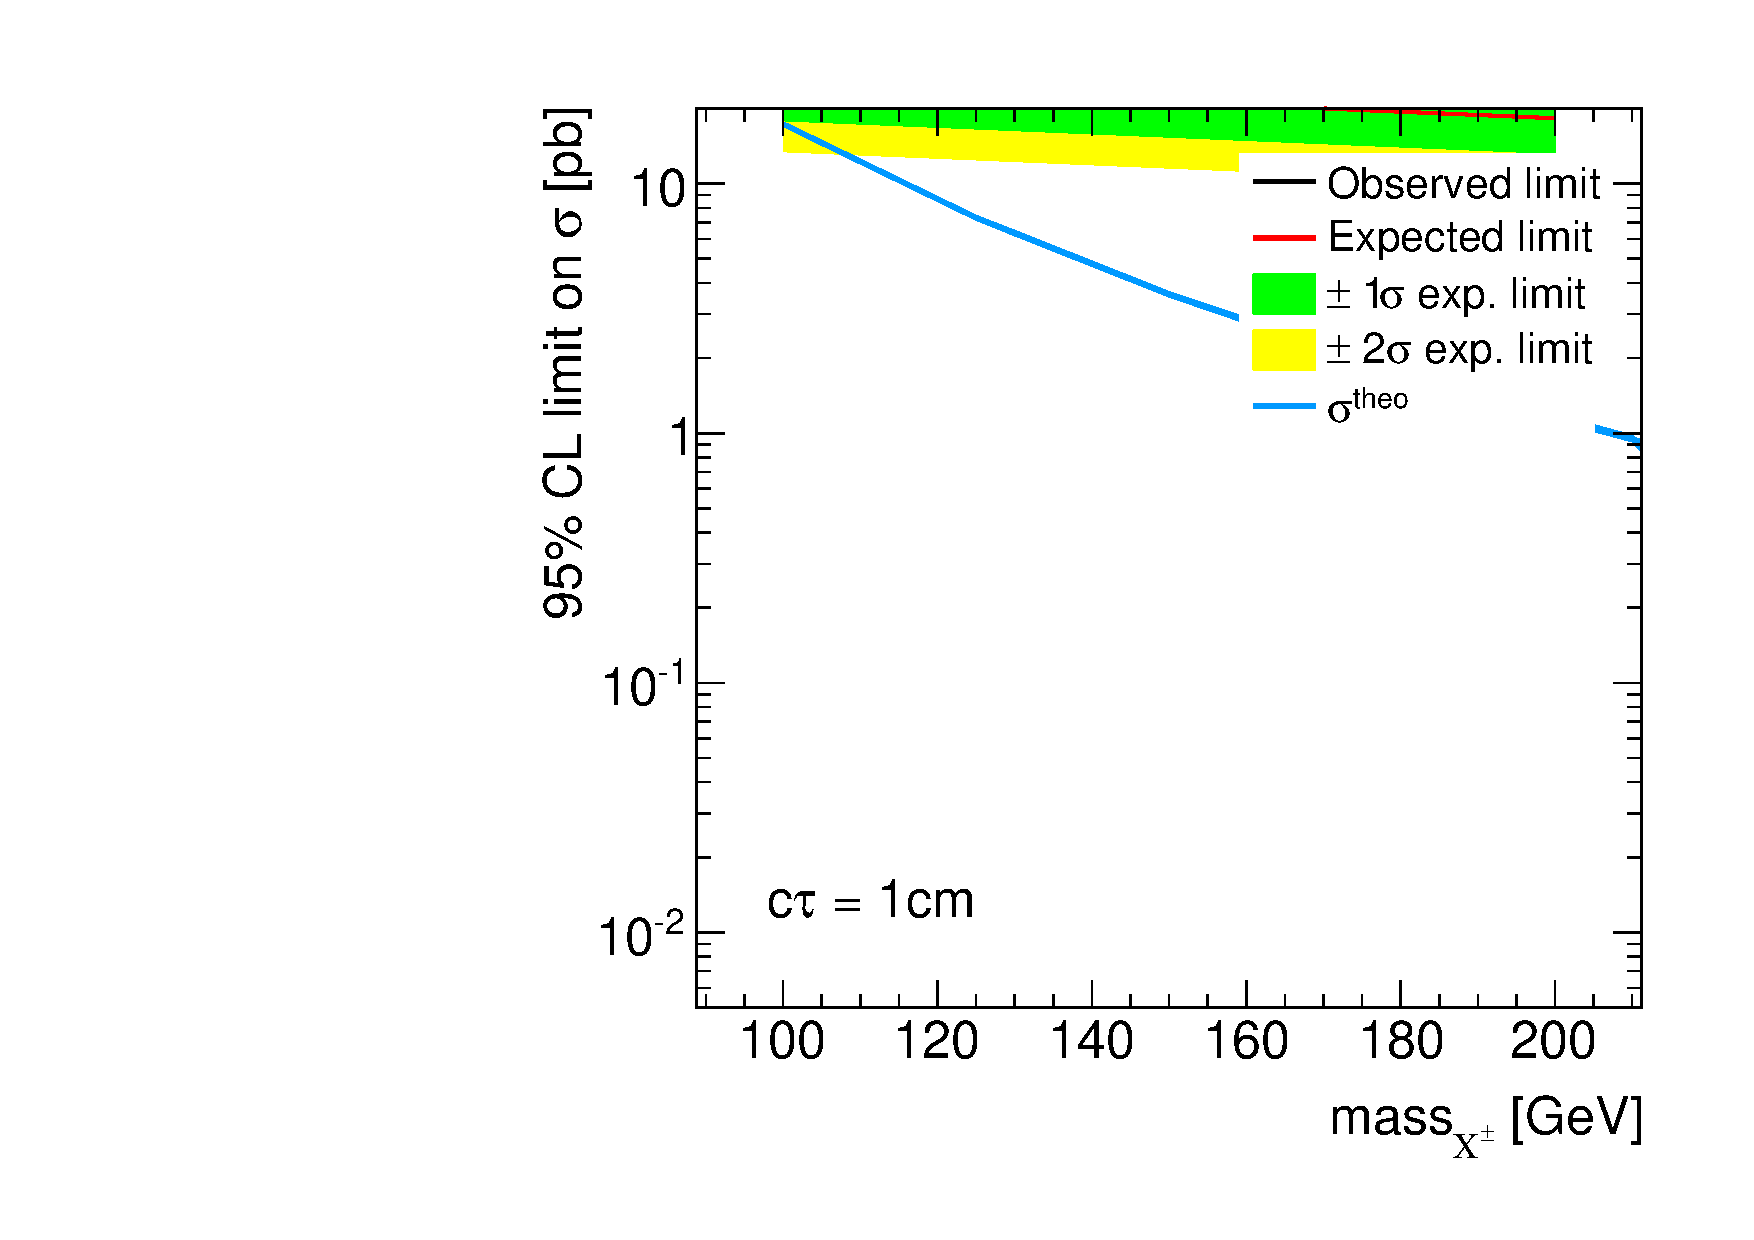
\includegraphics[width=0.29\textwidth]{figures/analysis/Interpretation/ExclusionLimits/LimitPlot_ctau1cm.pdf} 
    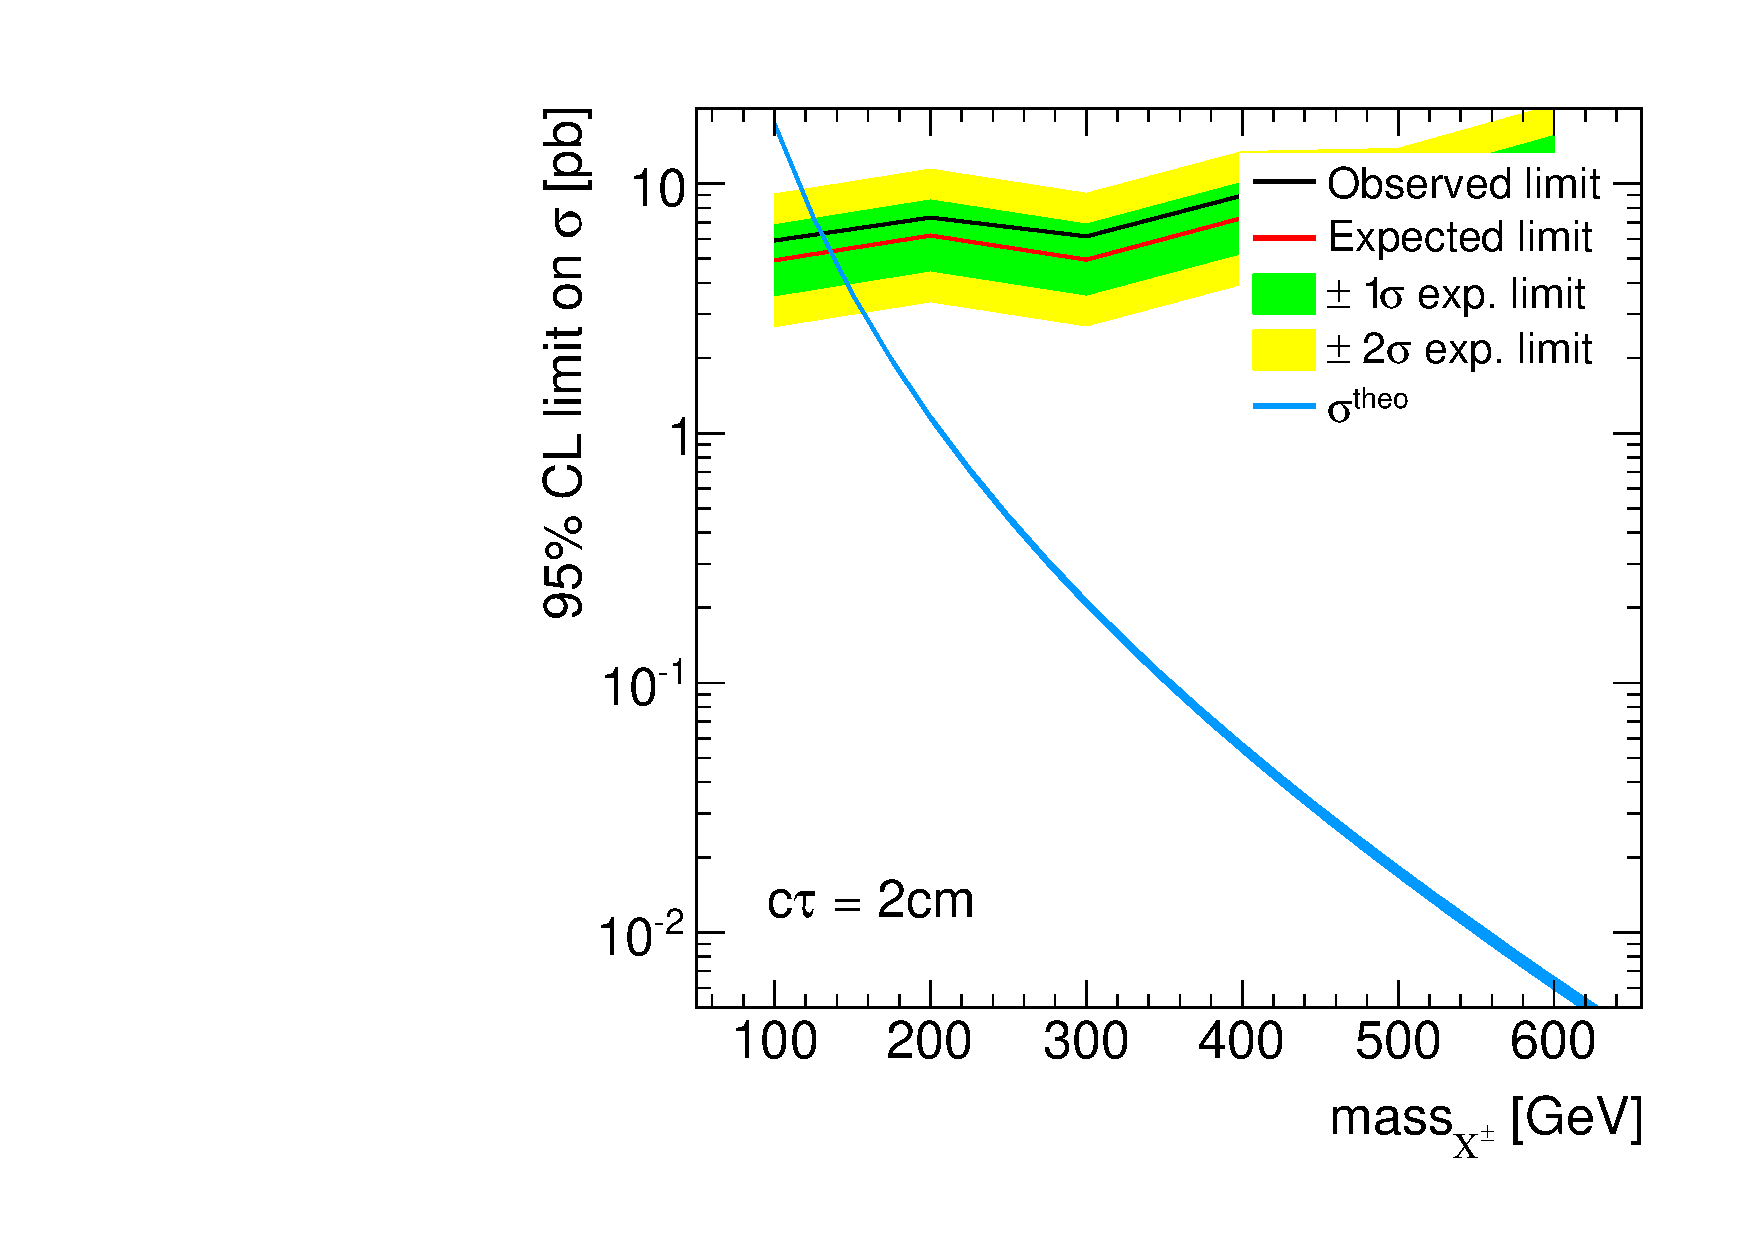
\includegraphics[width=0.29\textwidth]{figures/analysis/Interpretation/ExclusionLimits/LimitPlot_ctau2cm.pdf} 
    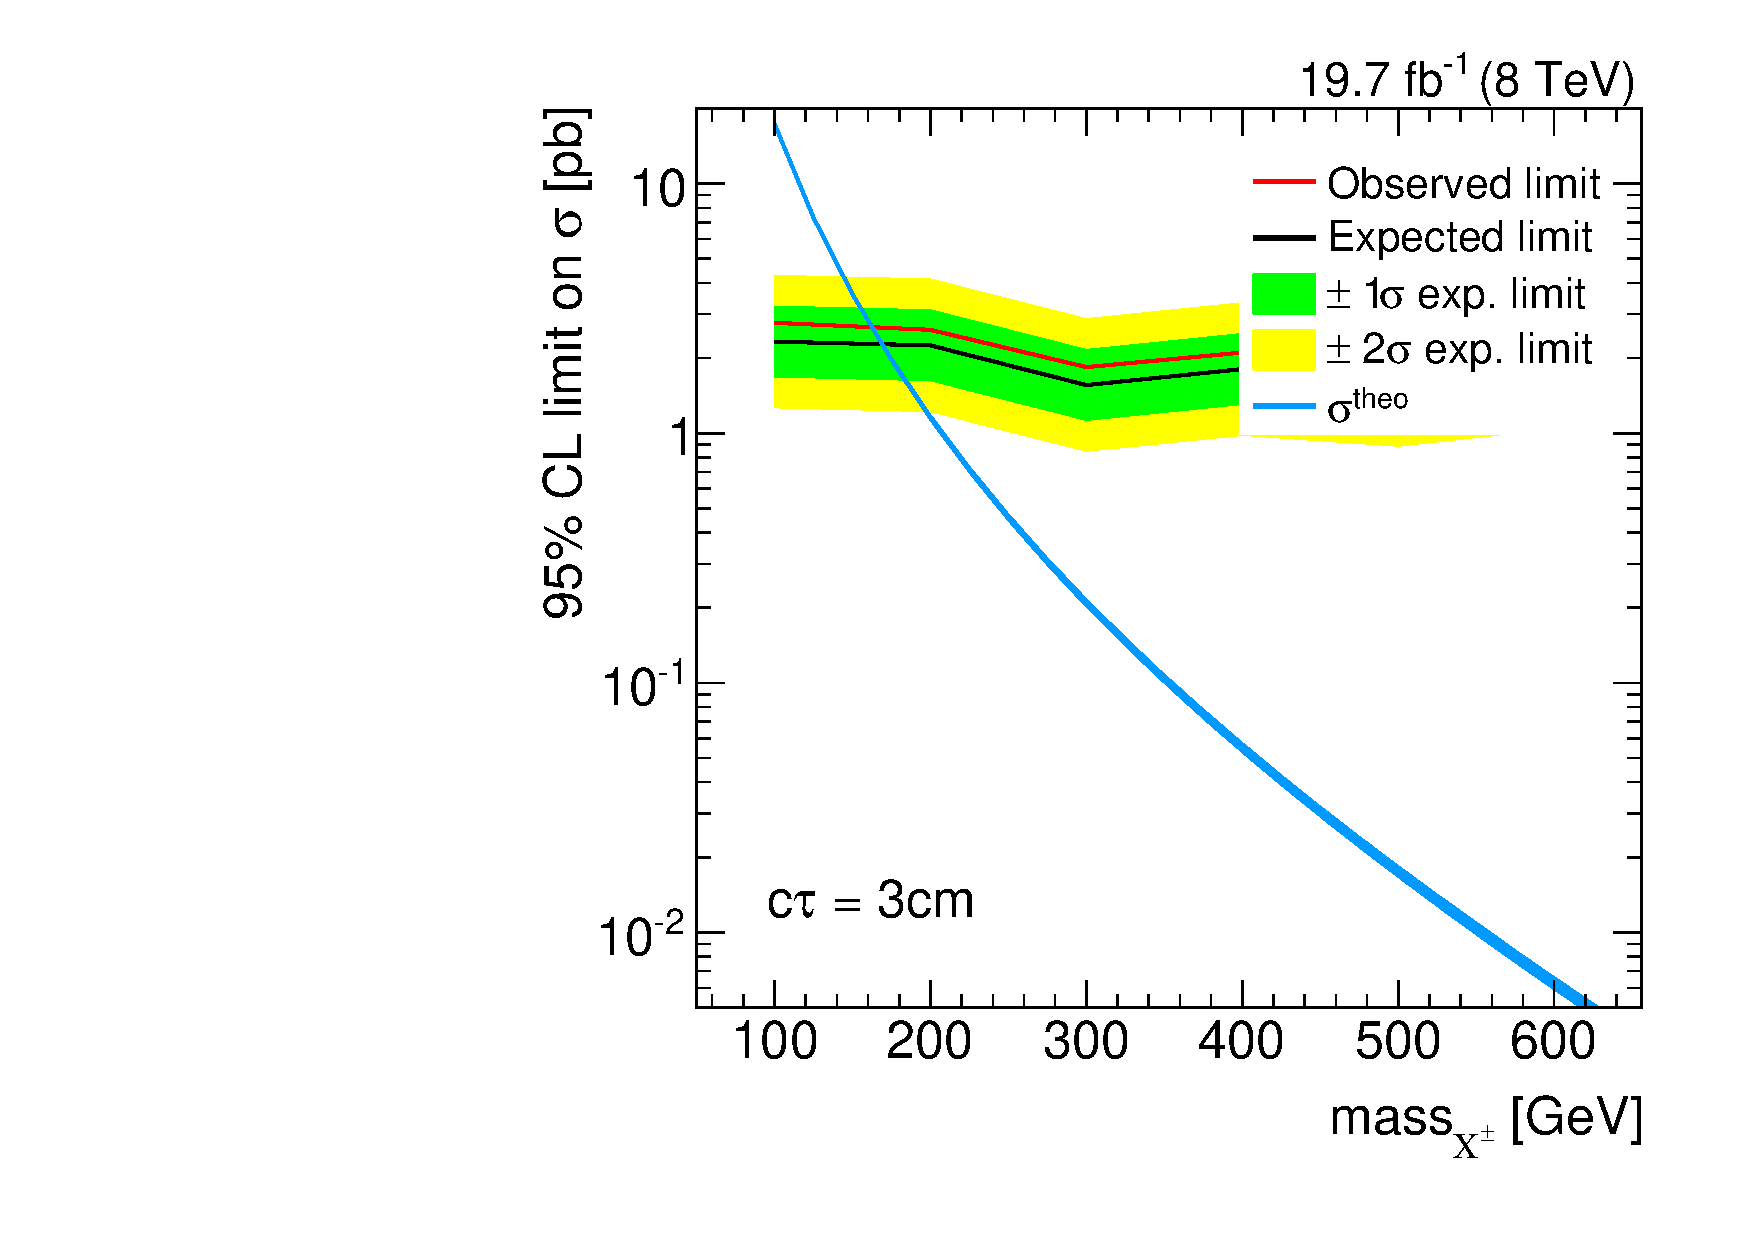
\includegraphics[width=0.29\textwidth]{figures/analysis/Interpretation/ExclusionLimits/LimitPlot_ctau3cm.pdf} \\
    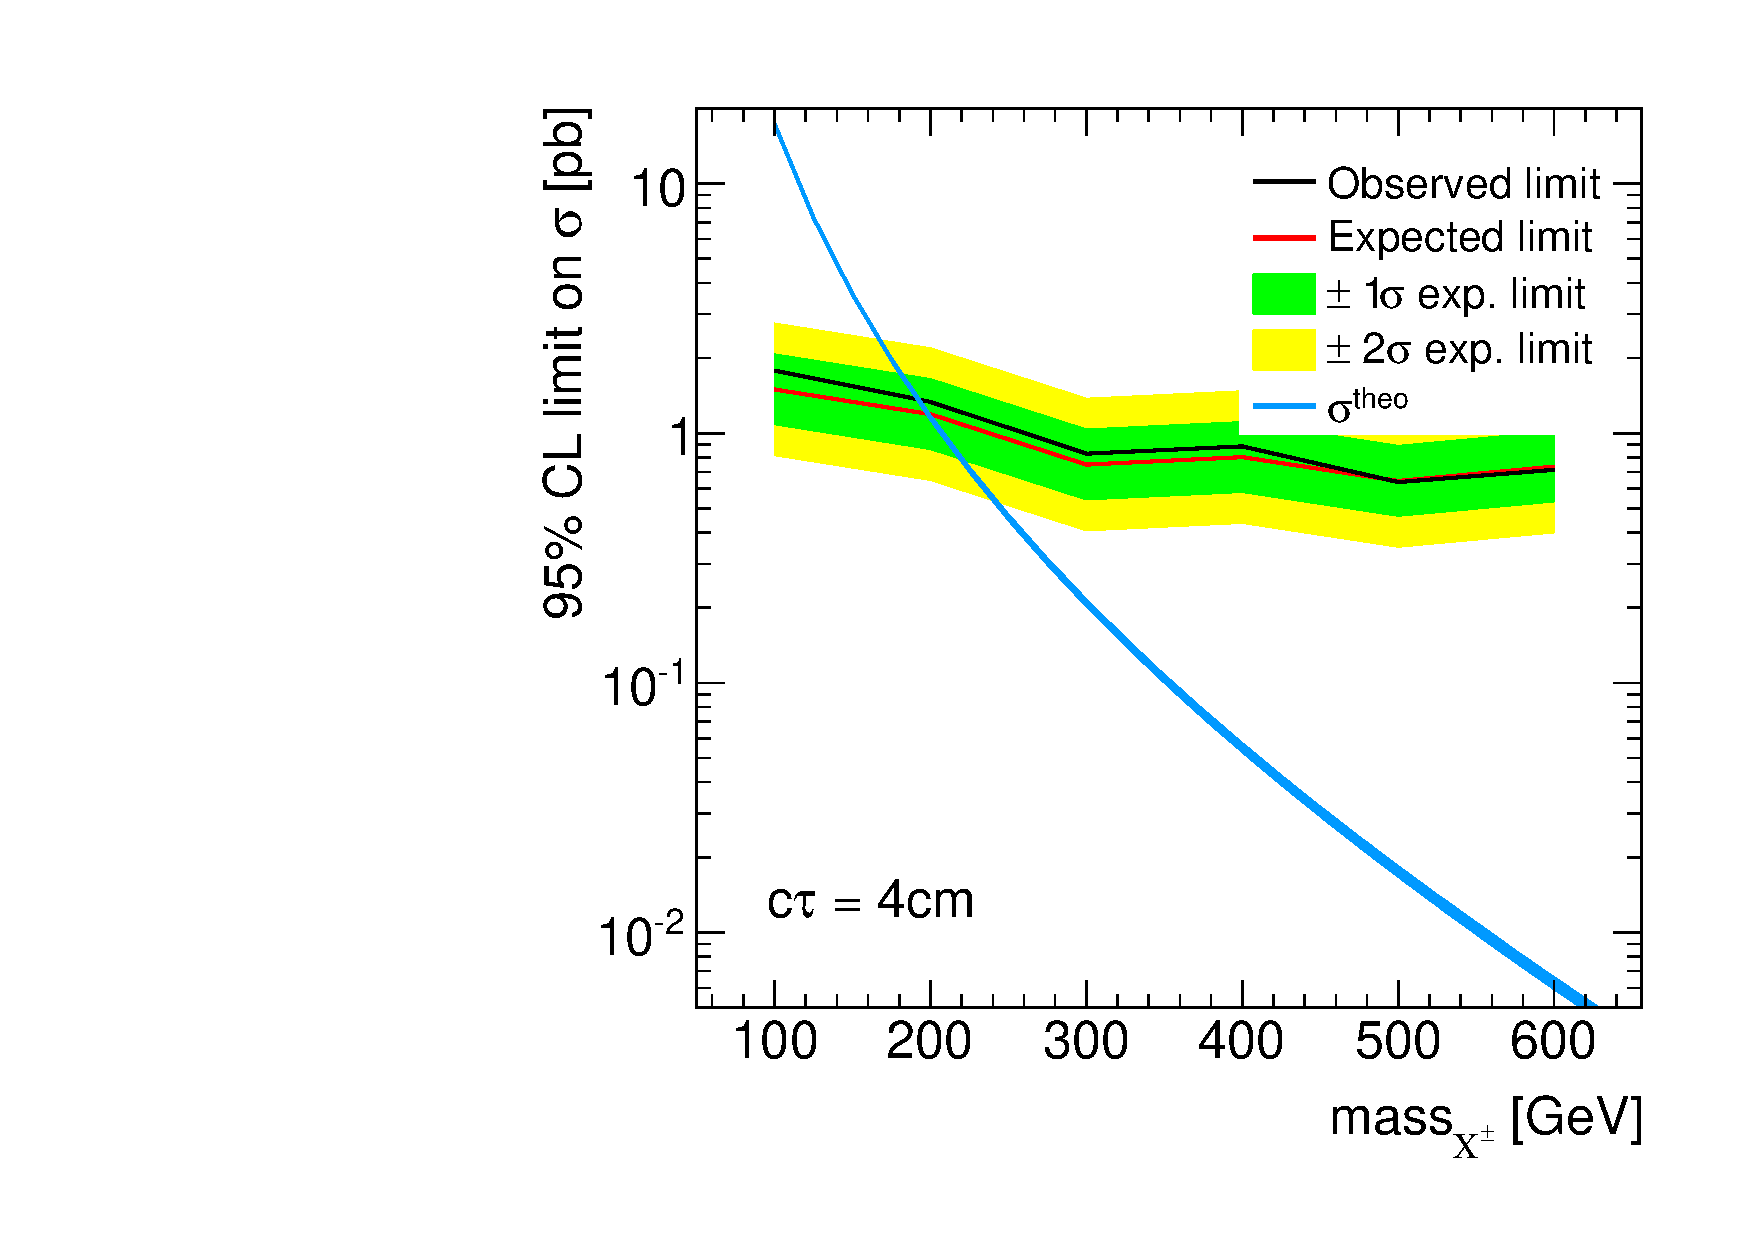
\includegraphics[width=0.29\textwidth]{figures/analysis/Interpretation/ExclusionLimits/LimitPlot_ctau4cm.pdf} 
    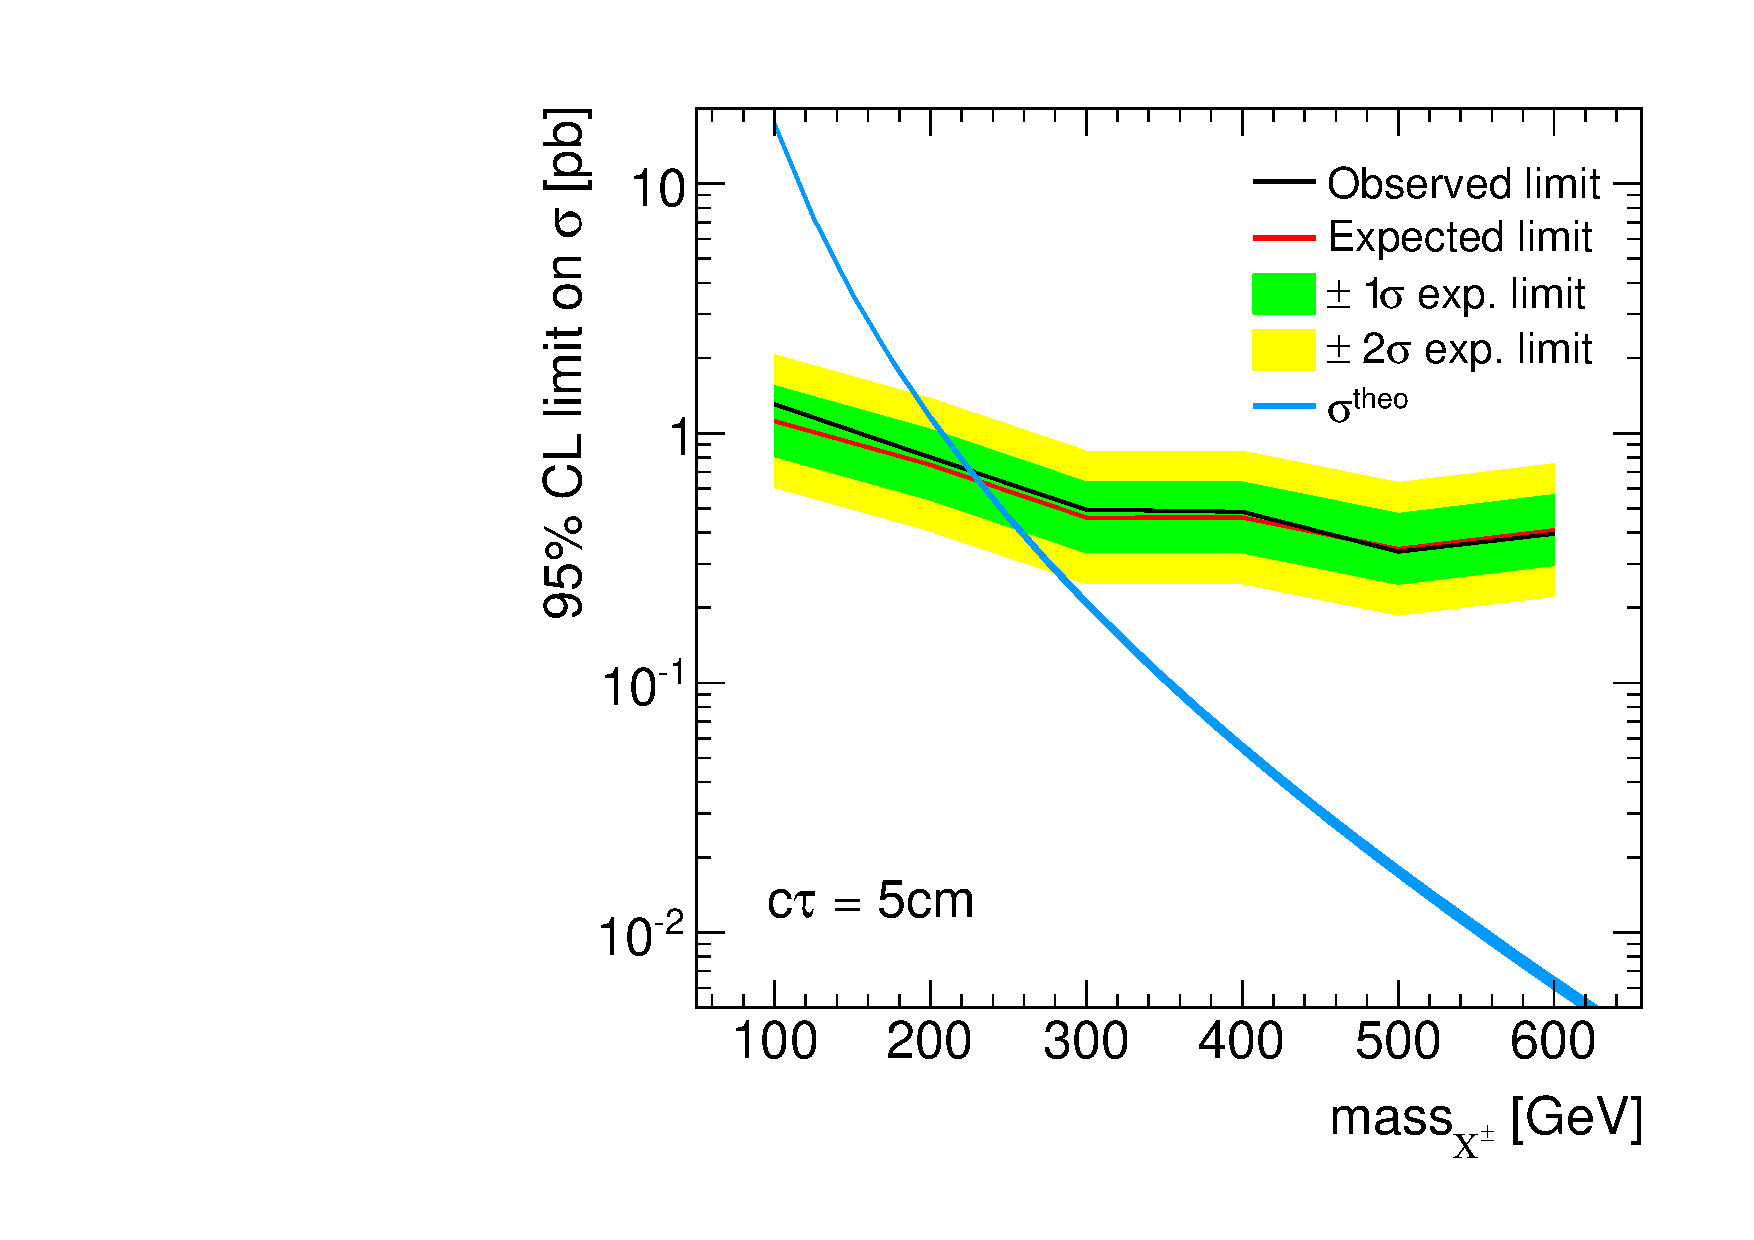
\includegraphics[width=0.29\textwidth]{figures/analysis/Interpretation/ExclusionLimits/LimitPlot_ctau5cm.pdf} 
    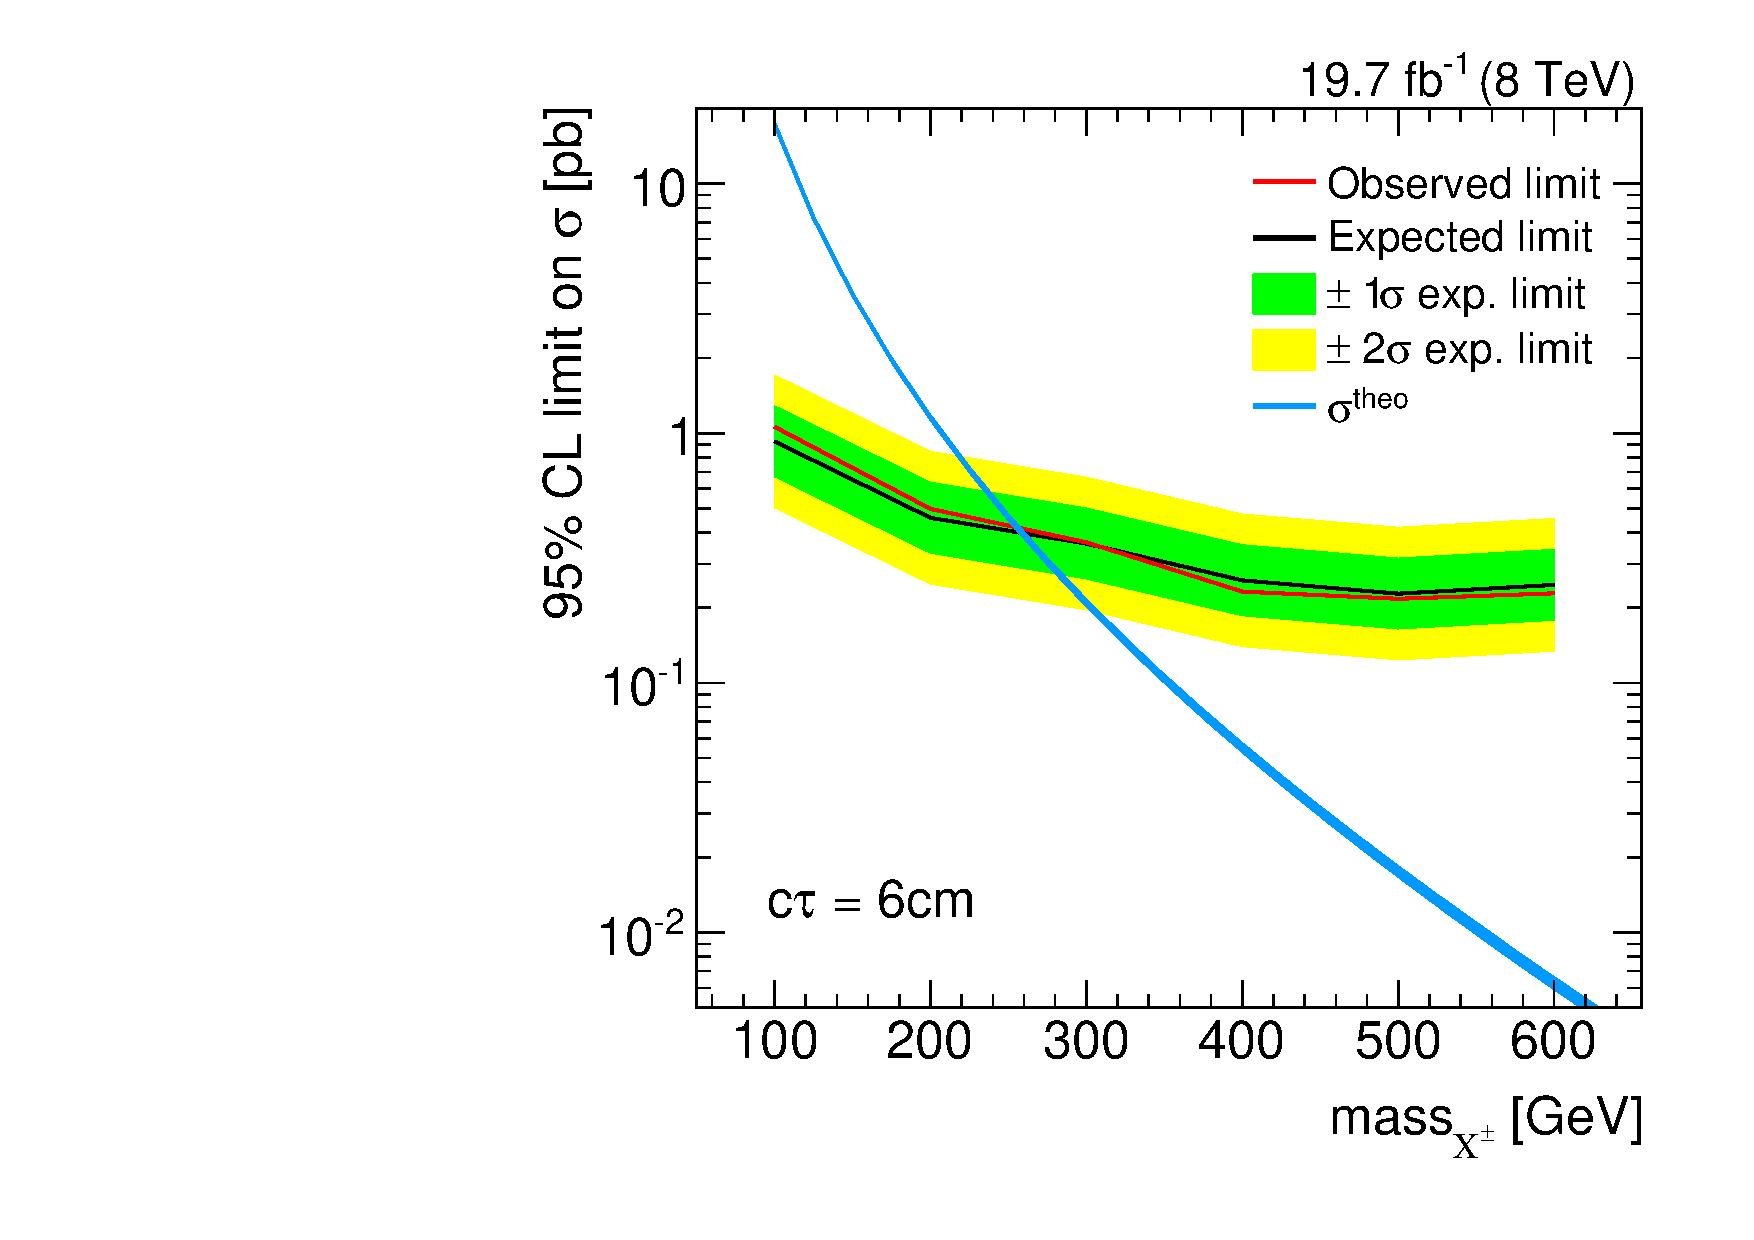
\includegraphics[width=0.29\textwidth]{figures/analysis/Interpretation/ExclusionLimits/LimitPlot_ctau6cm.pdf} \\
    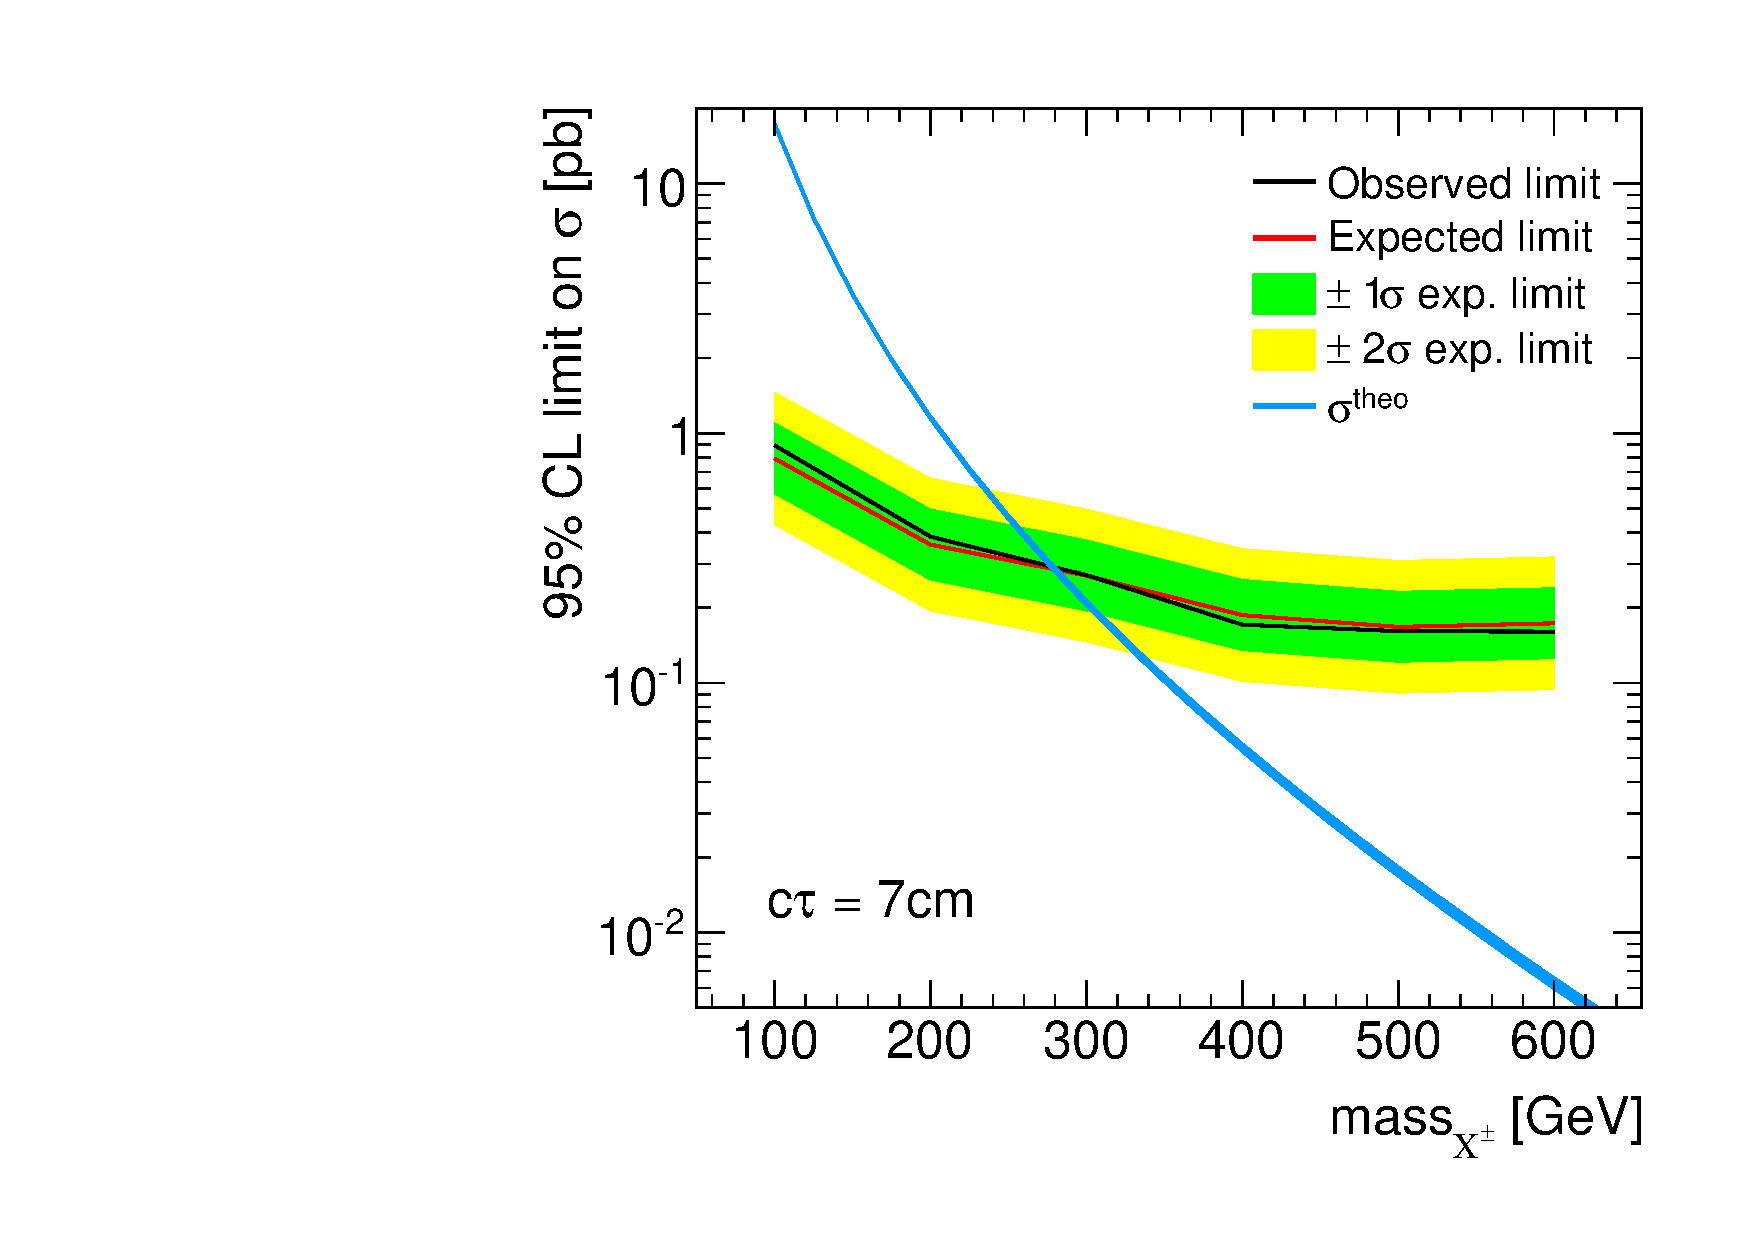
\includegraphics[width=0.29\textwidth]{figures/analysis/Interpretation/ExclusionLimits/LimitPlot_ctau7cm.pdf} 
    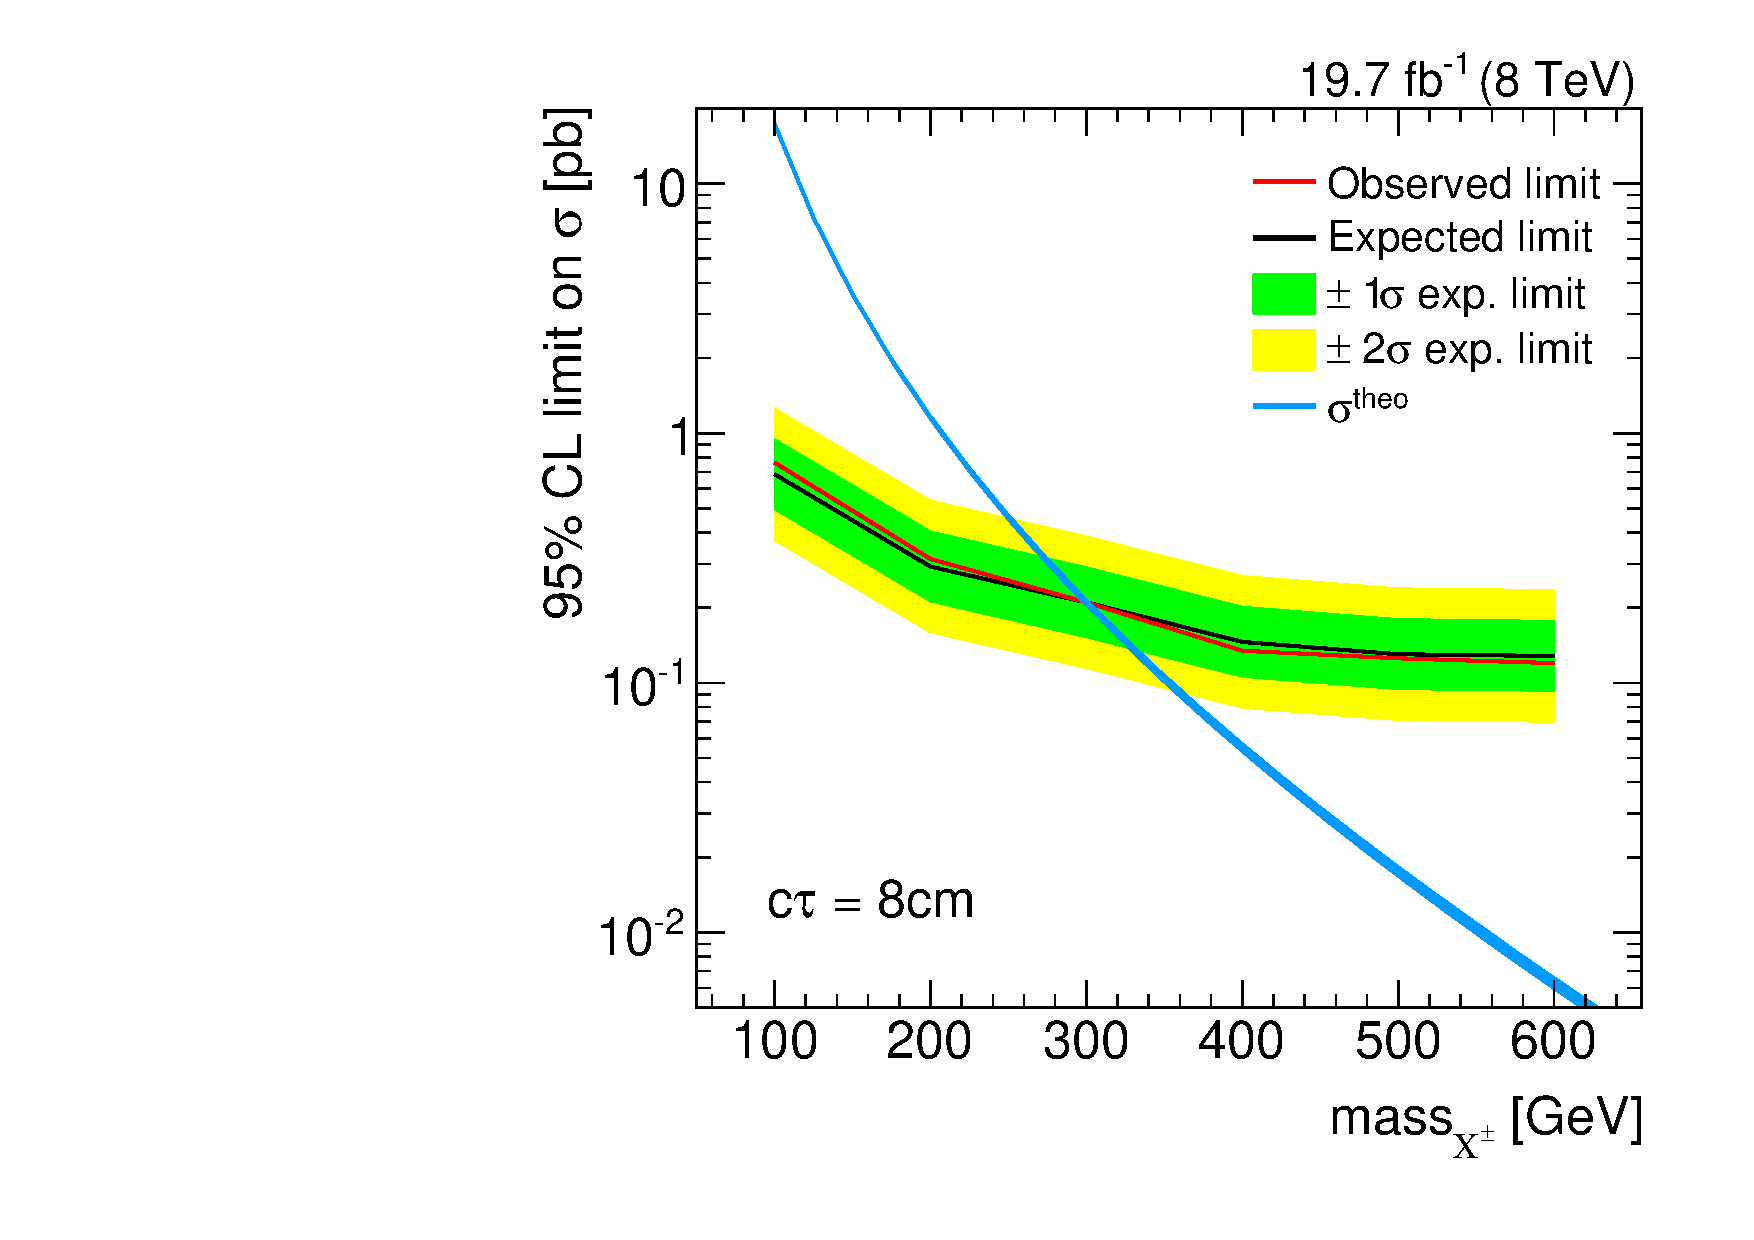
\includegraphics[width=0.29\textwidth]{figures/analysis/Interpretation/ExclusionLimits/LimitPlot_ctau8cm.pdf} 
    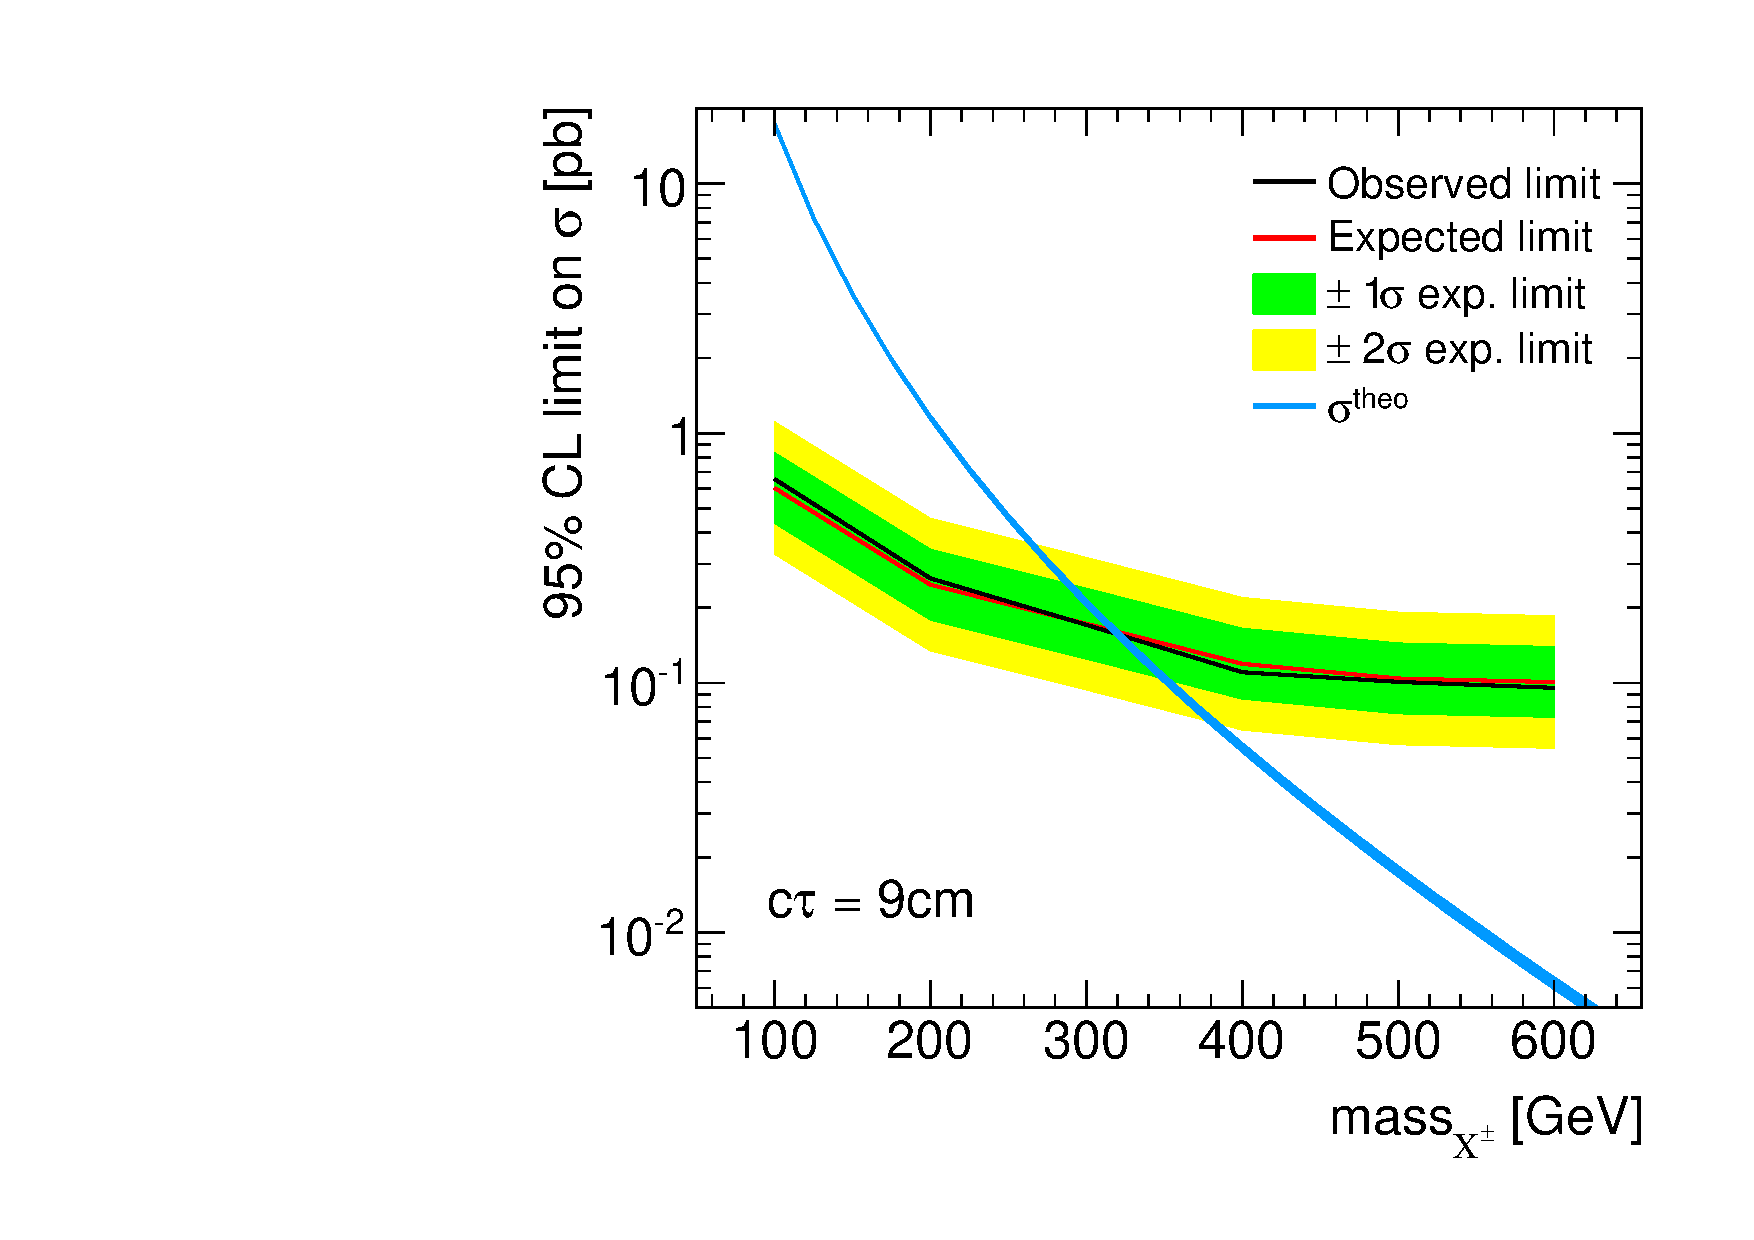
\includegraphics[width=0.29\textwidth]{figures/analysis/Interpretation/ExclusionLimits/LimitPlot_ctau9cm.pdf} \\
    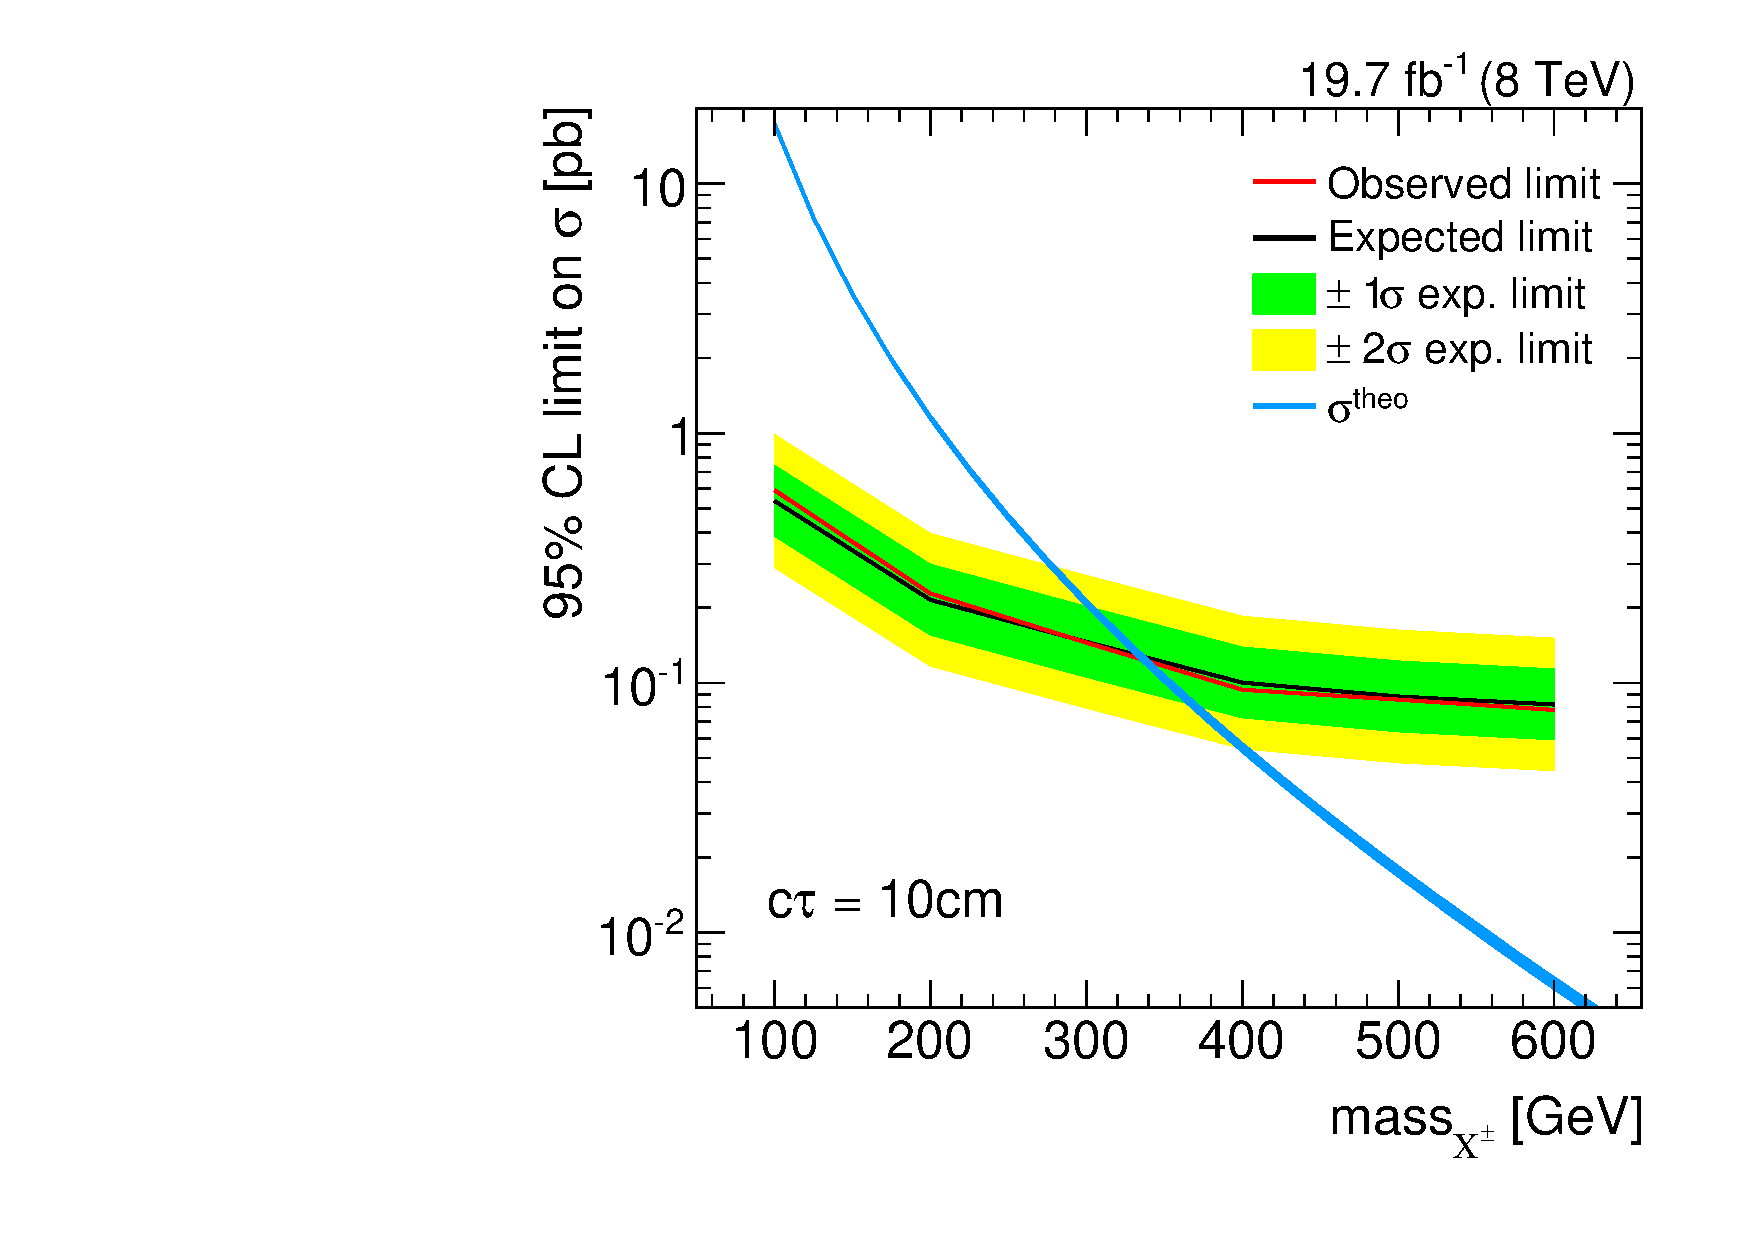
\includegraphics[width=0.29\textwidth]{figures/analysis/Interpretation/ExclusionLimits/LimitPlot_ctau10cm.pdf} 
    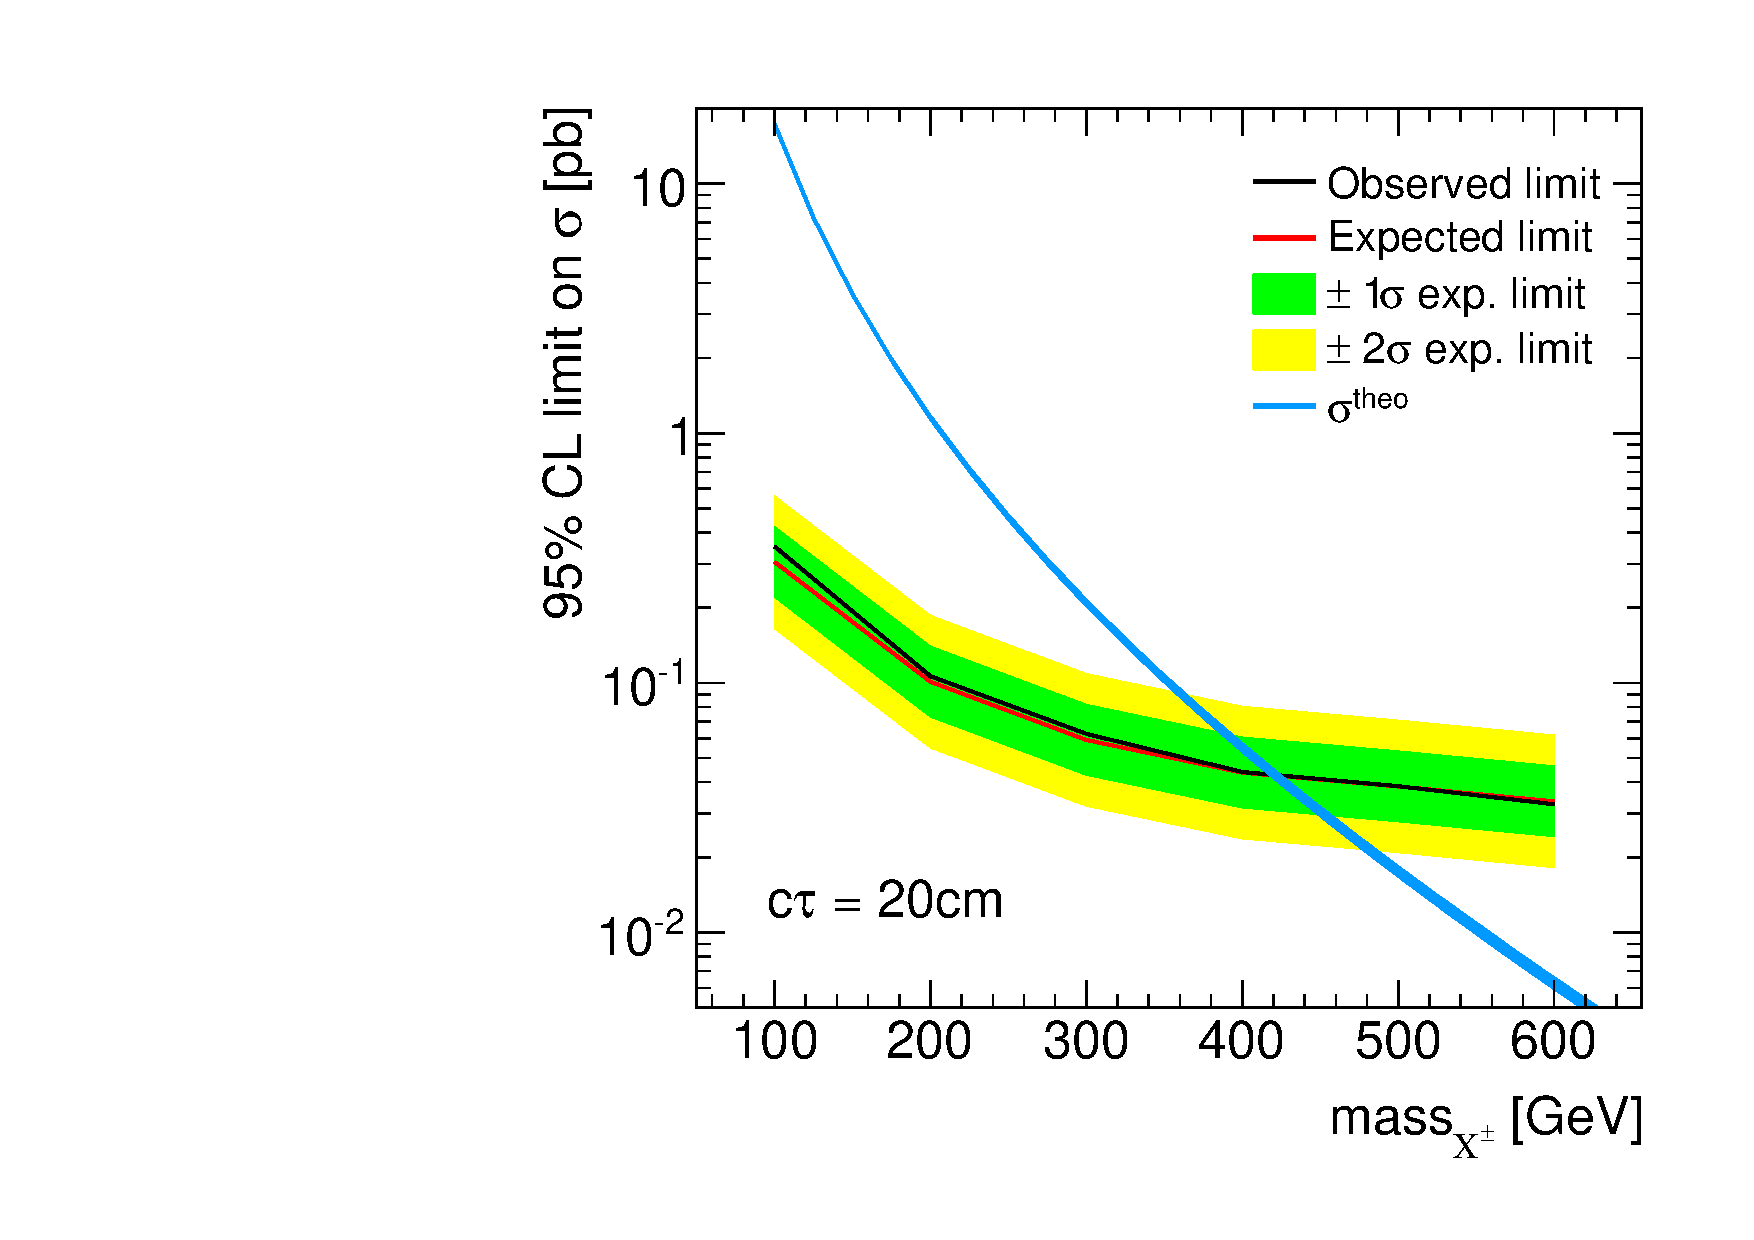
\includegraphics[width=0.29\textwidth]{figures/analysis/Interpretation/ExclusionLimits/LimitPlot_ctau20cm.pdf} 
    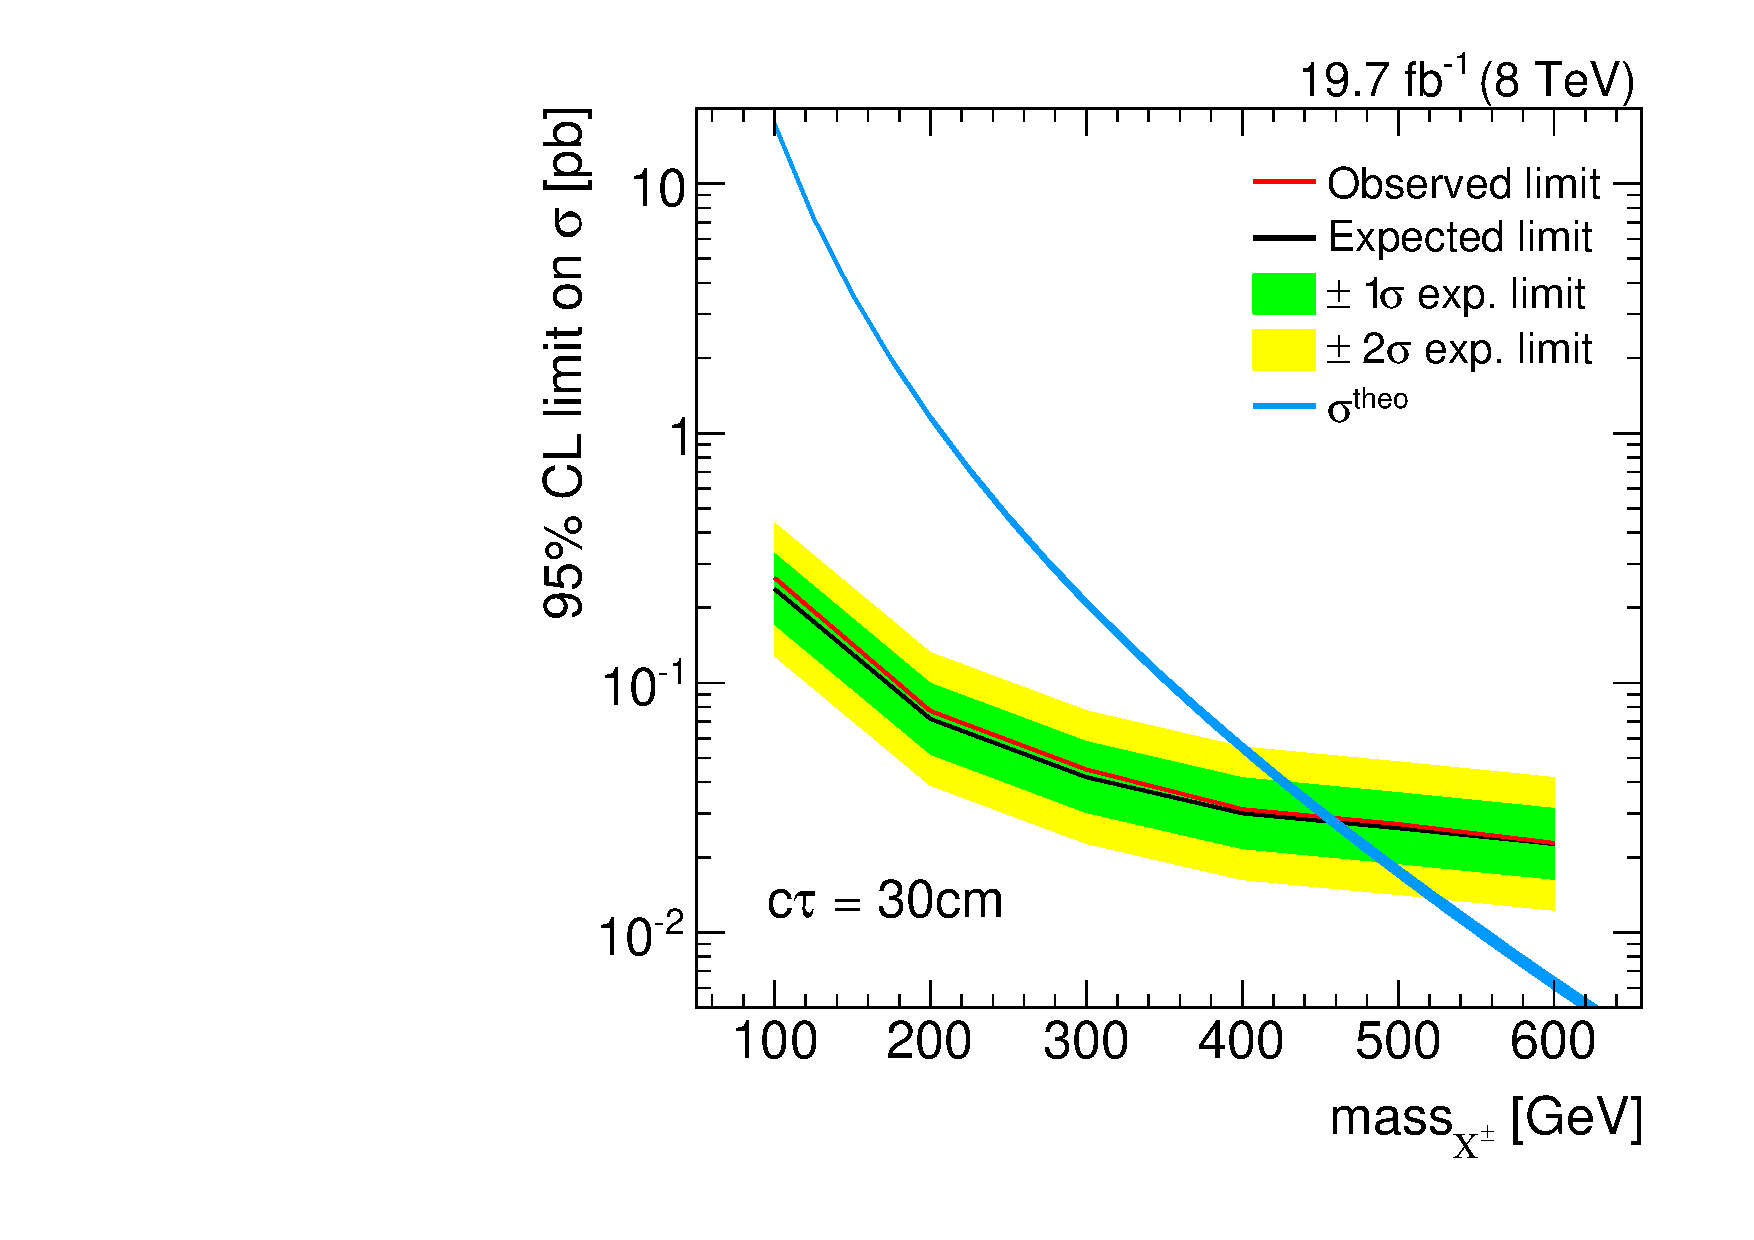
\includegraphics[width=0.29\textwidth]{figures/analysis/Interpretation/ExclusionLimits/LimitPlot_ctau30cm.pdf} \\
  \end{tabular}
  \caption{95\% CL exclusion limits for signal models with $\ctau = 1-30\cm$.}
  \label{fig:1dLimitsA}
\end{figure}

\begin{figure}[!h]
  \centering 
  \begin{tabular}{c}
    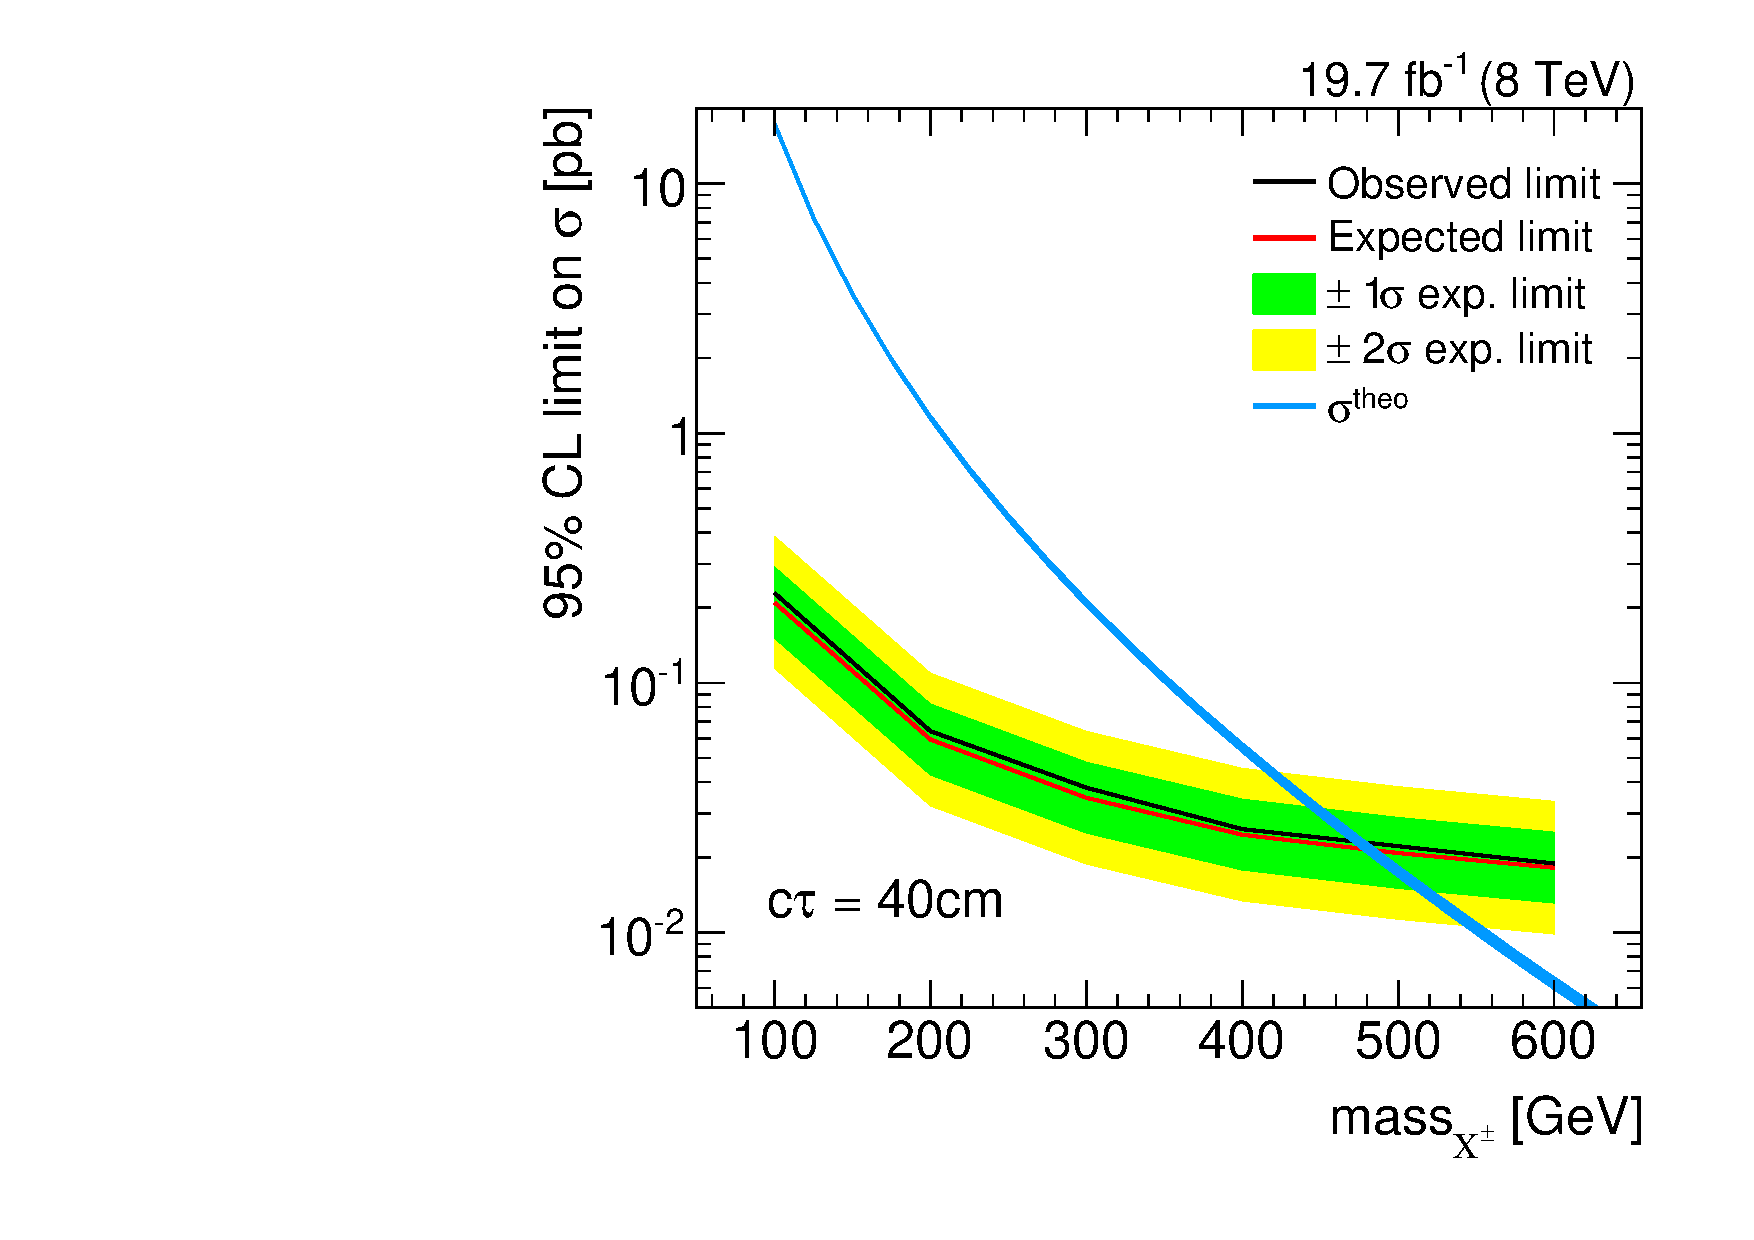
\includegraphics[width=0.29\textwidth]{figures/analysis/Interpretation/ExclusionLimits/LimitPlot_ctau40cm.pdf} 
    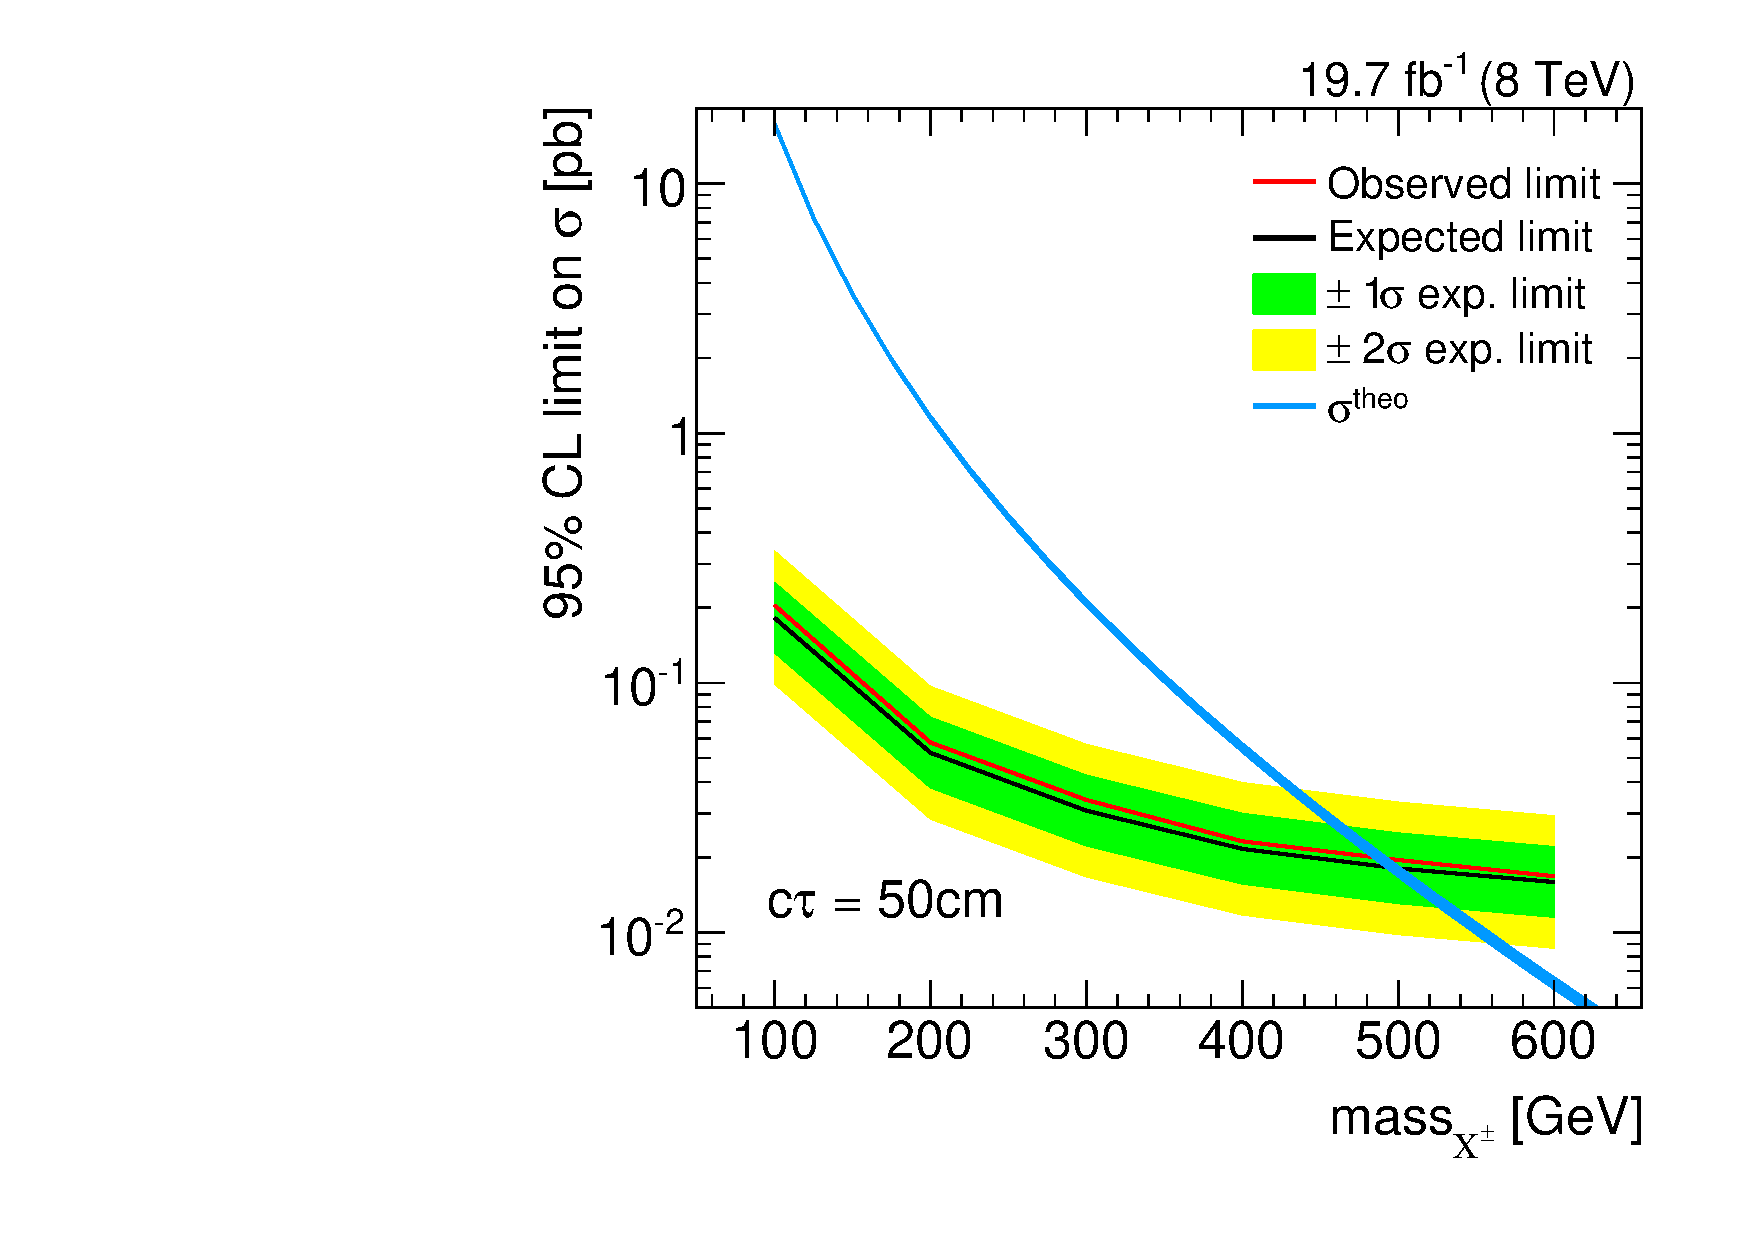
\includegraphics[width=0.29\textwidth]{figures/analysis/Interpretation/ExclusionLimits/LimitPlot_ctau50cm.pdf} 
    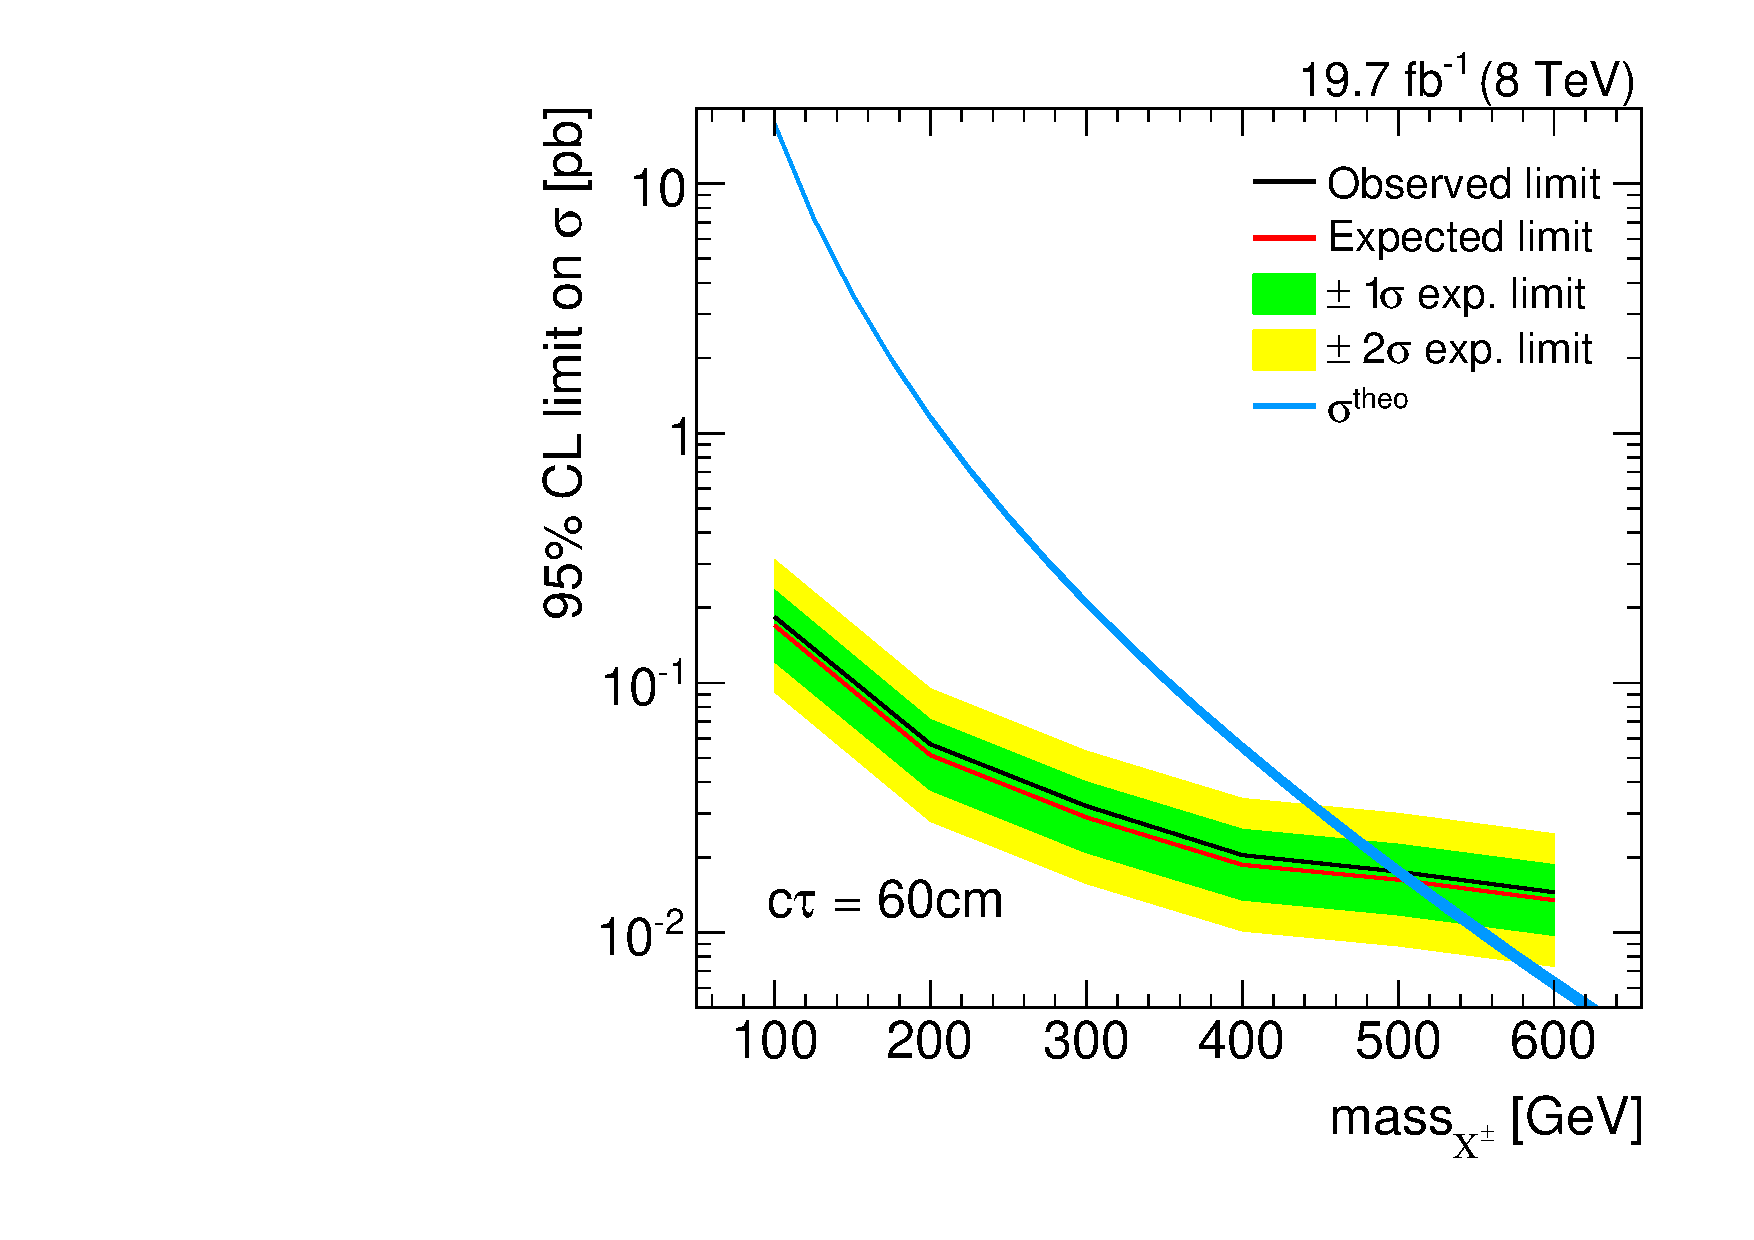
\includegraphics[width=0.29\textwidth]{figures/analysis/Interpretation/ExclusionLimits/LimitPlot_ctau60cm.pdf} \\
    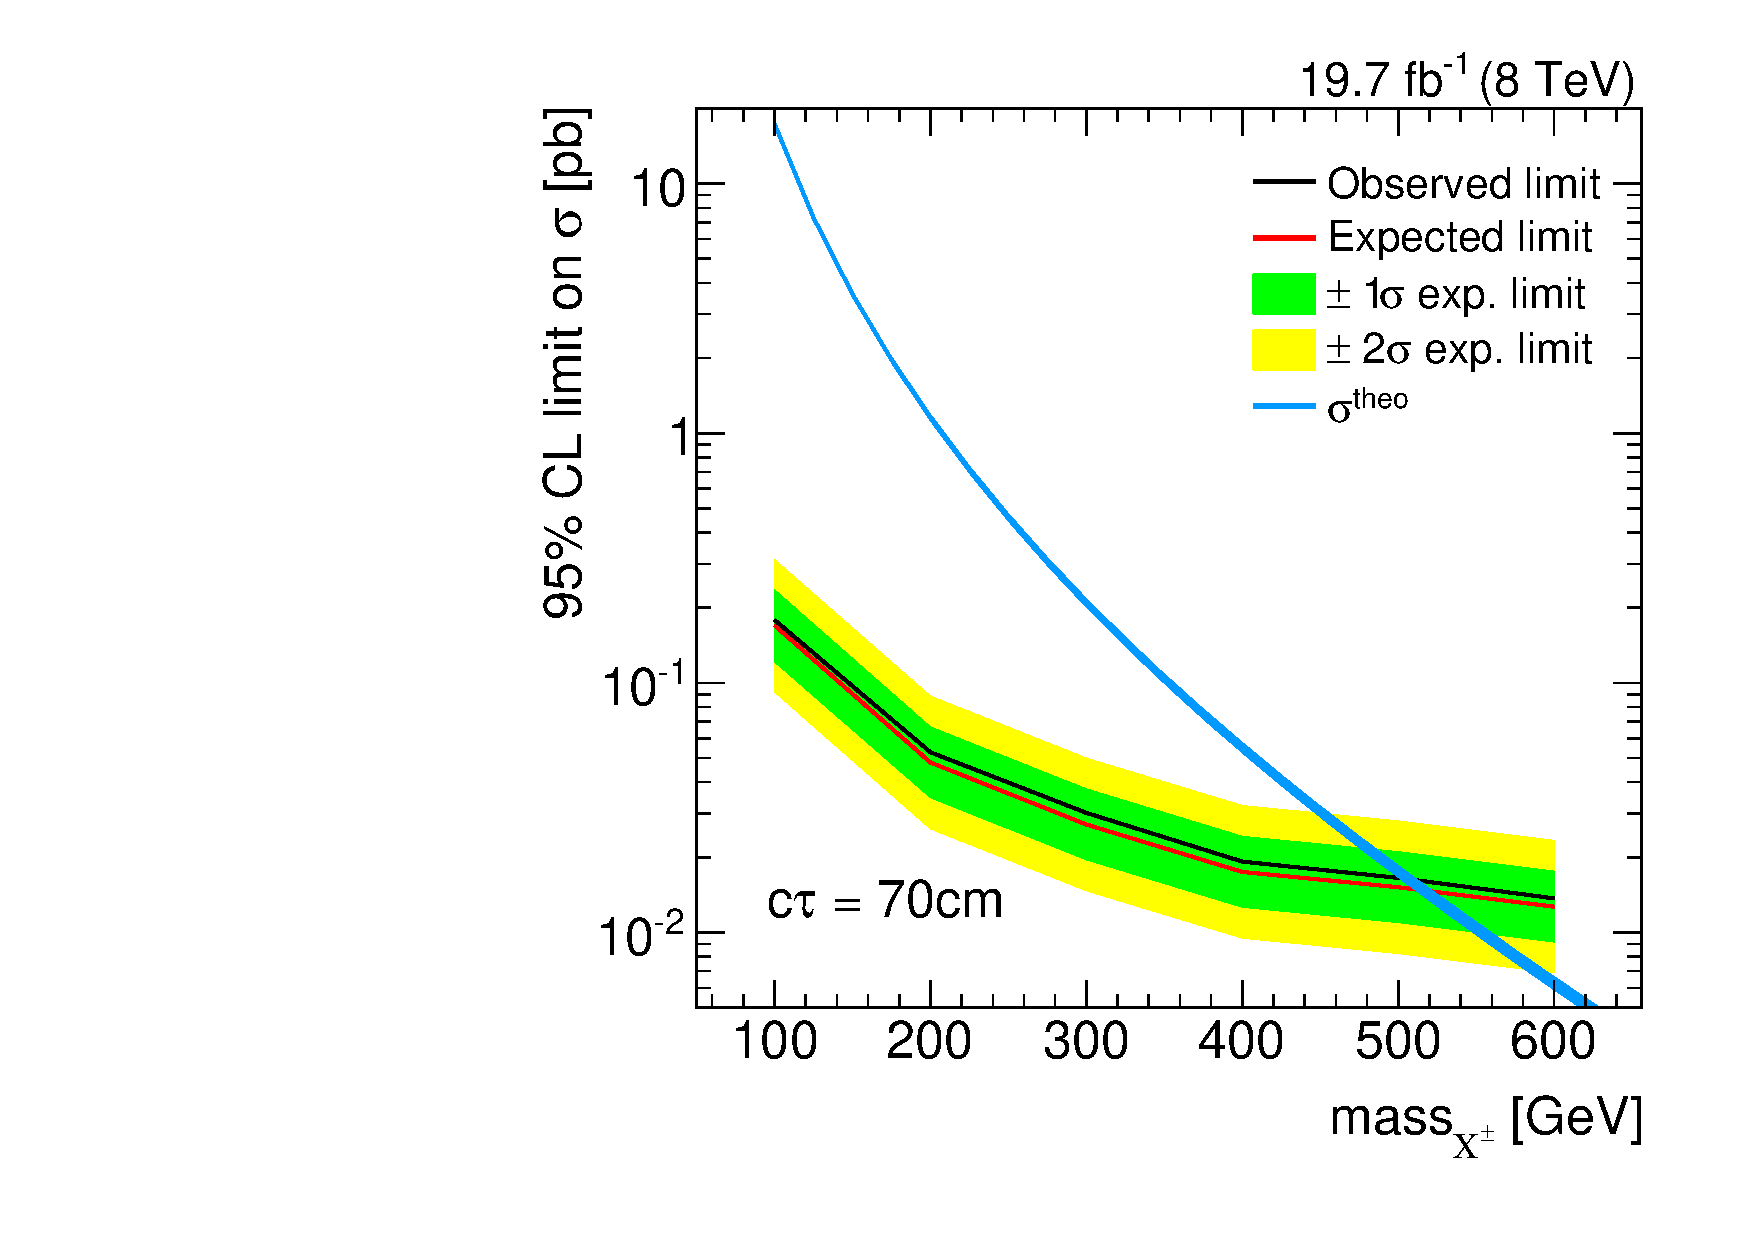
\includegraphics[width=0.29\textwidth]{figures/analysis/Interpretation/ExclusionLimits/LimitPlot_ctau70cm.pdf} 
    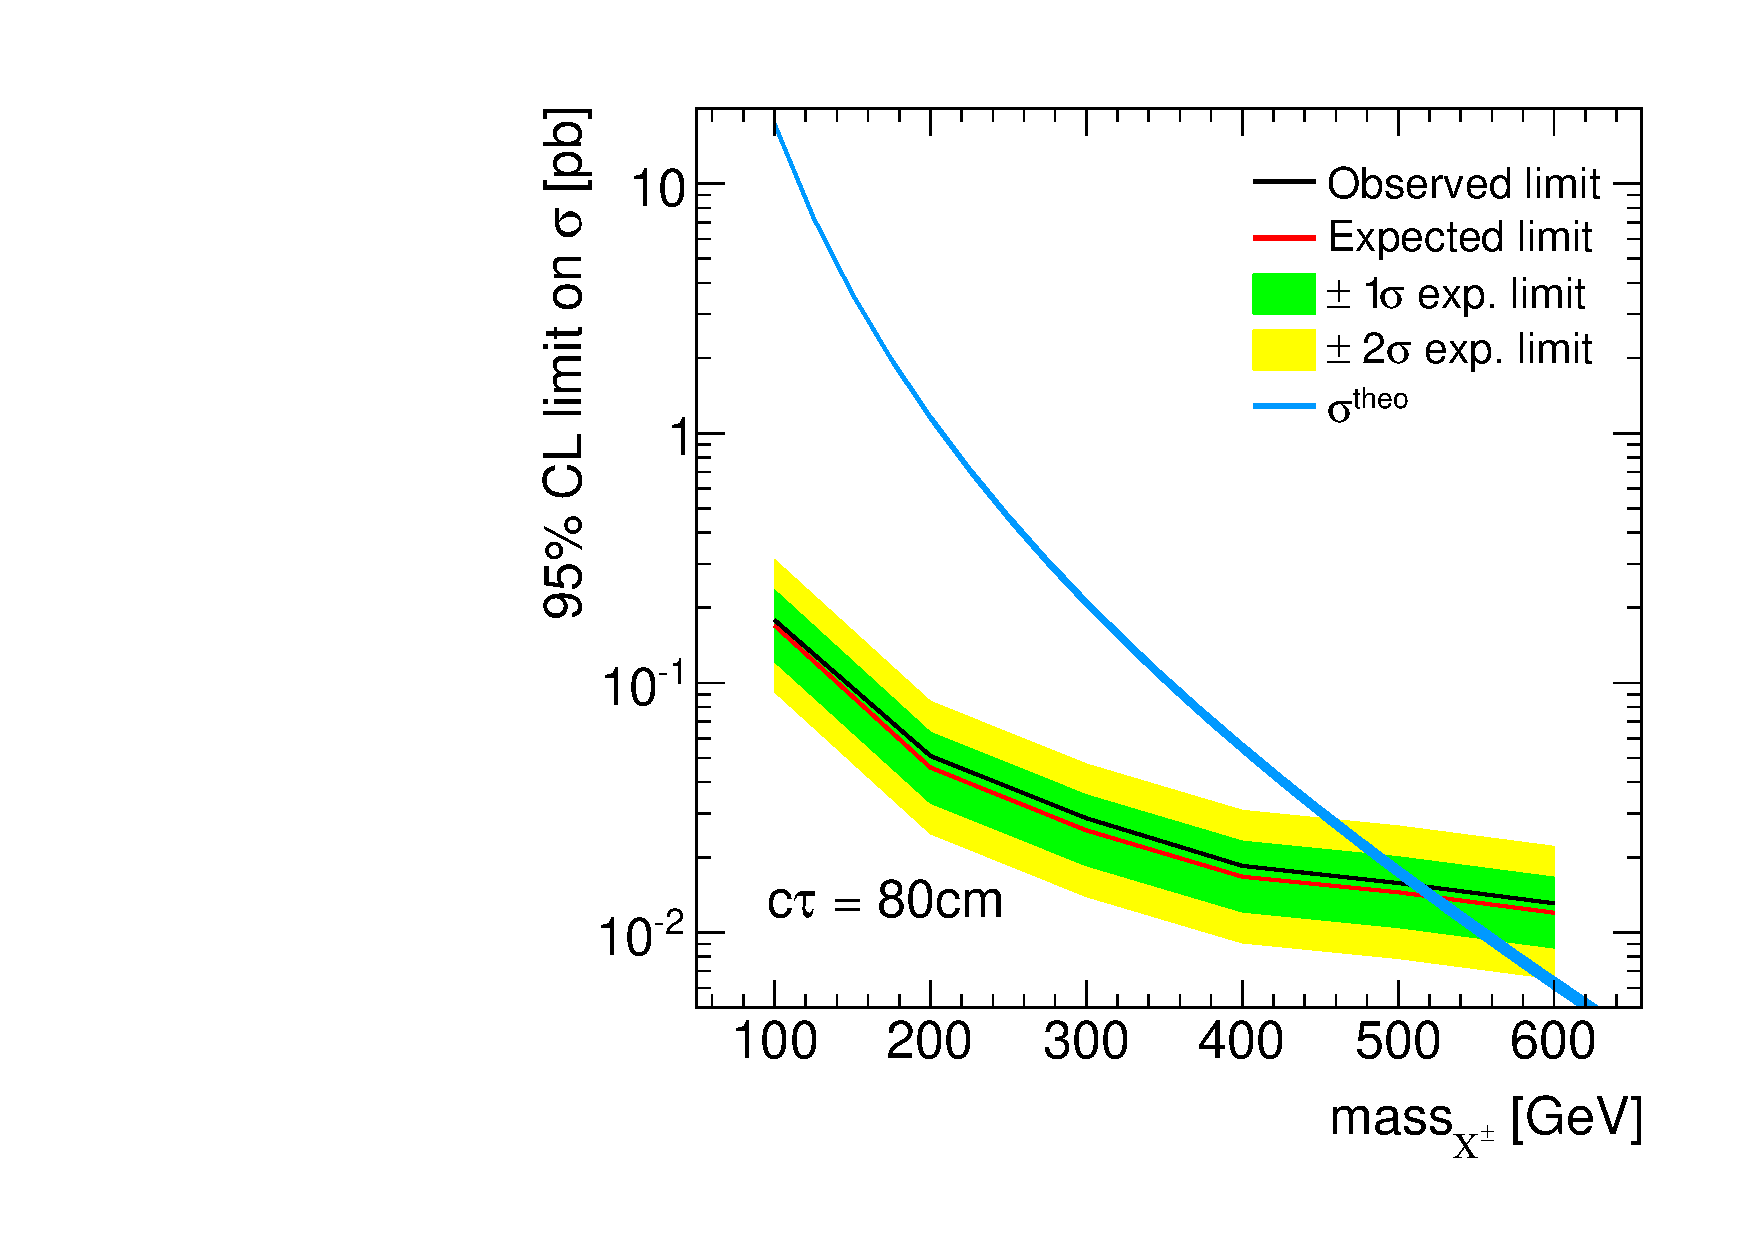
\includegraphics[width=0.29\textwidth]{figures/analysis/Interpretation/ExclusionLimits/LimitPlot_ctau80cm.pdf} 
    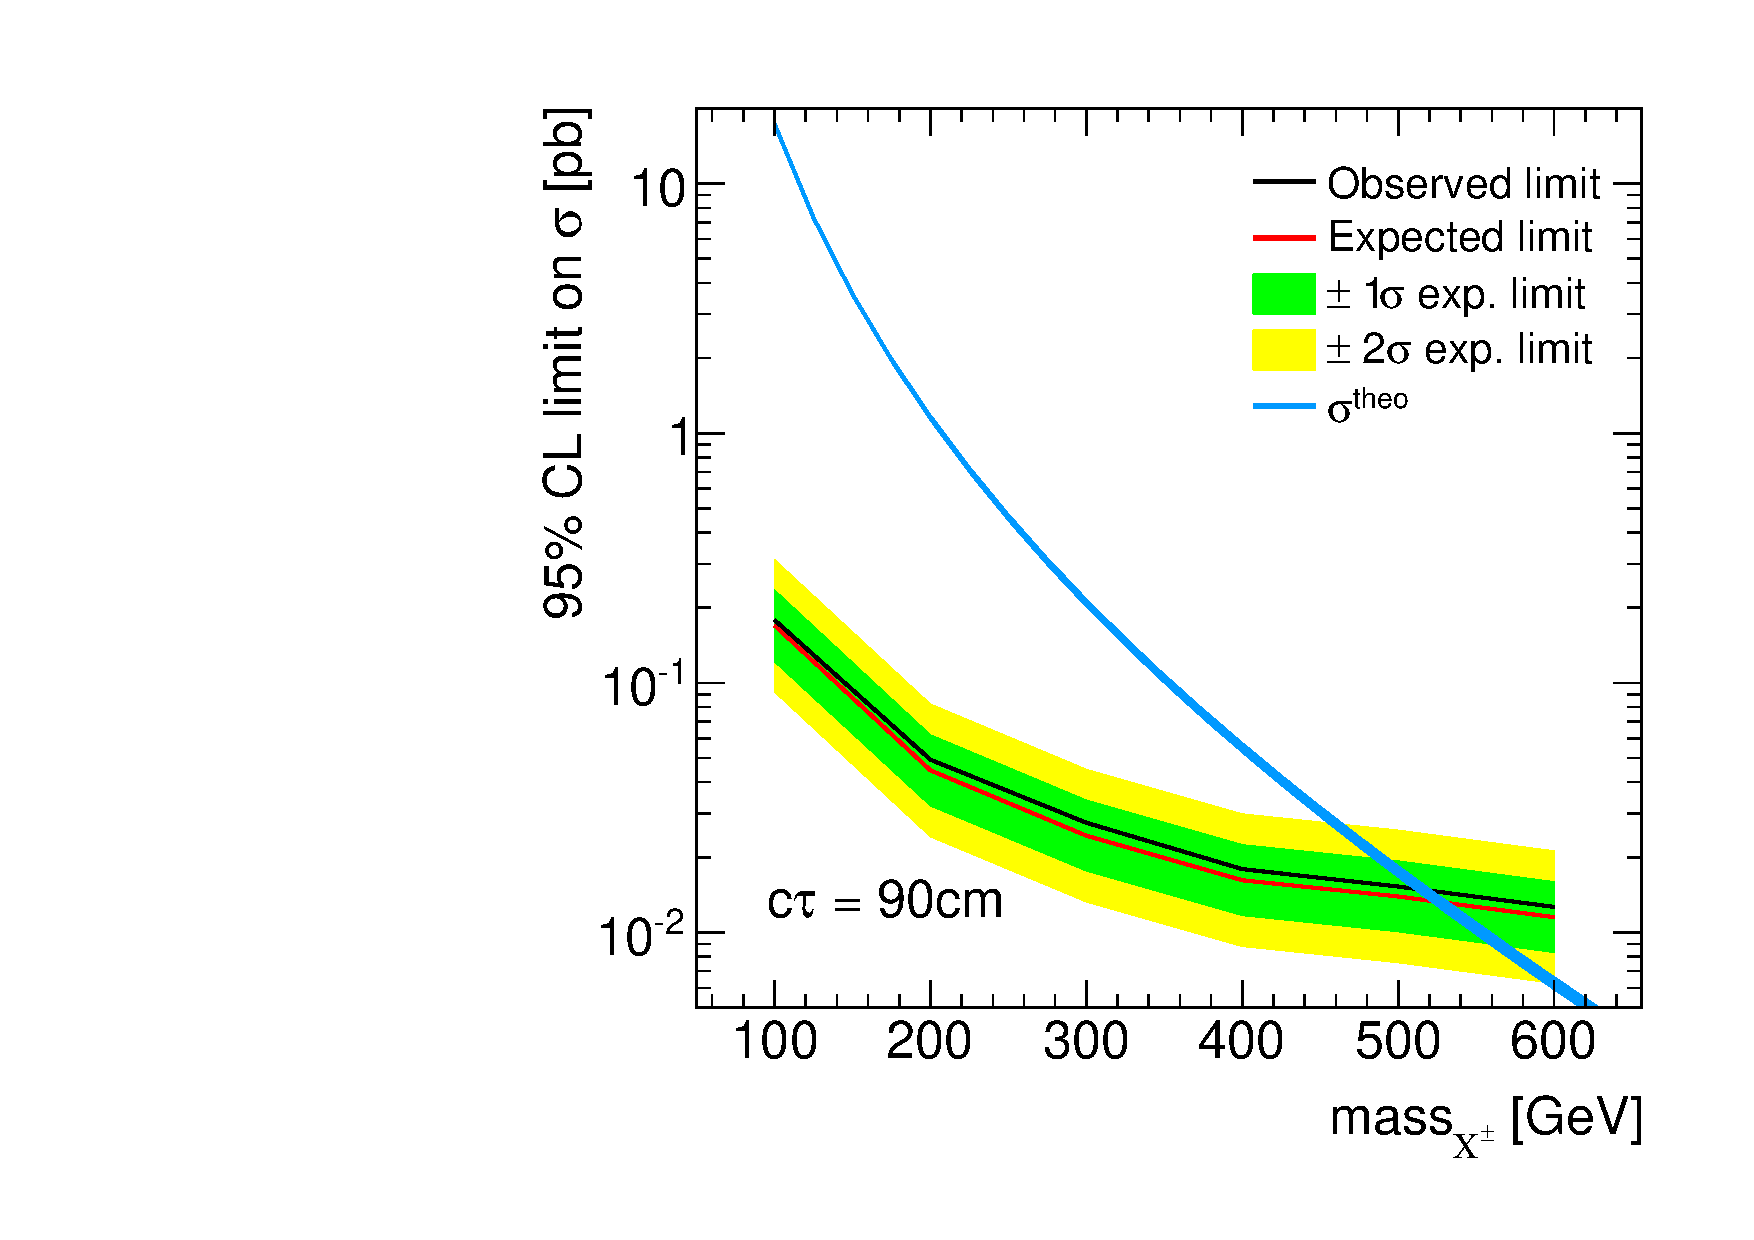
\includegraphics[width=0.29\textwidth]{figures/analysis/Interpretation/ExclusionLimits/LimitPlot_ctau90cm.pdf} \\
    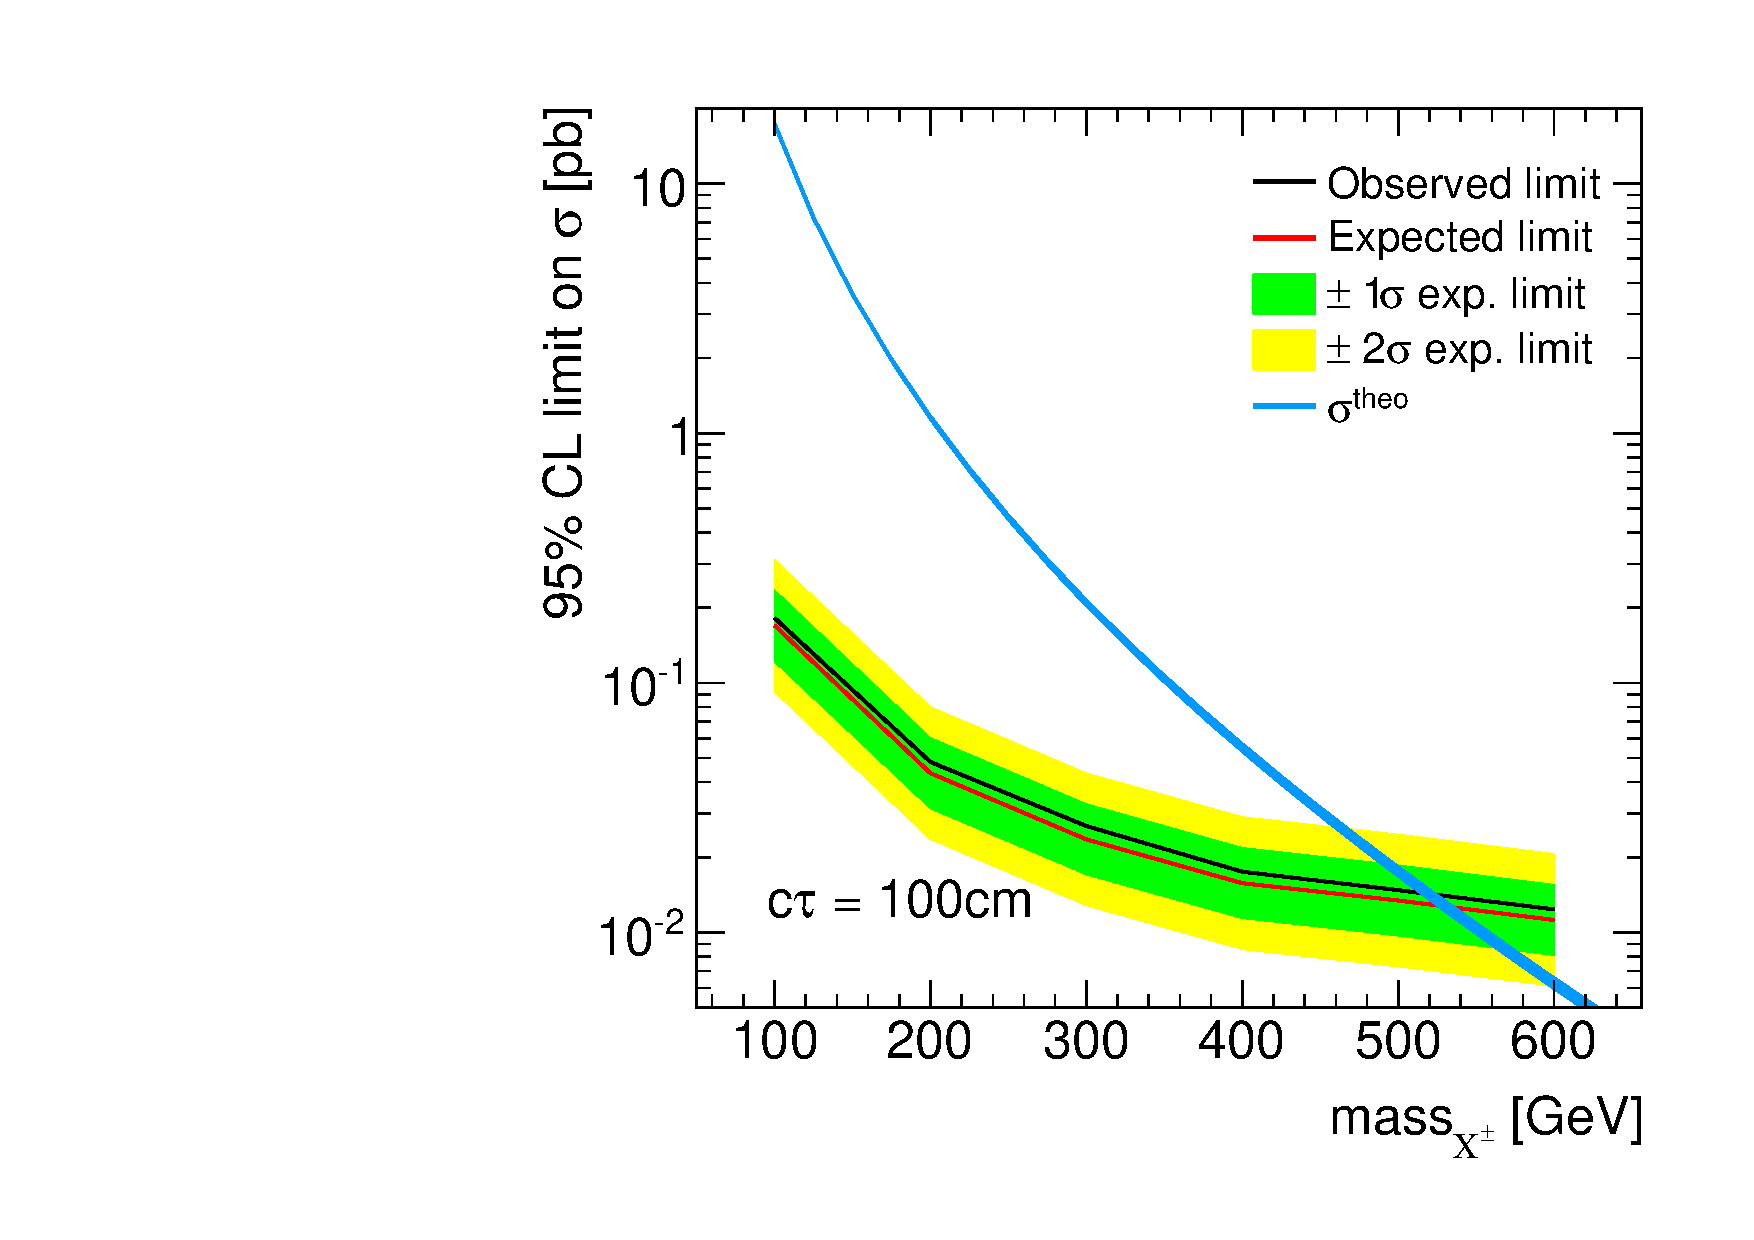
\includegraphics[width=0.29\textwidth]{figures/analysis/Interpretation/ExclusionLimits/LimitPlot_ctau100cm.pdf} 
    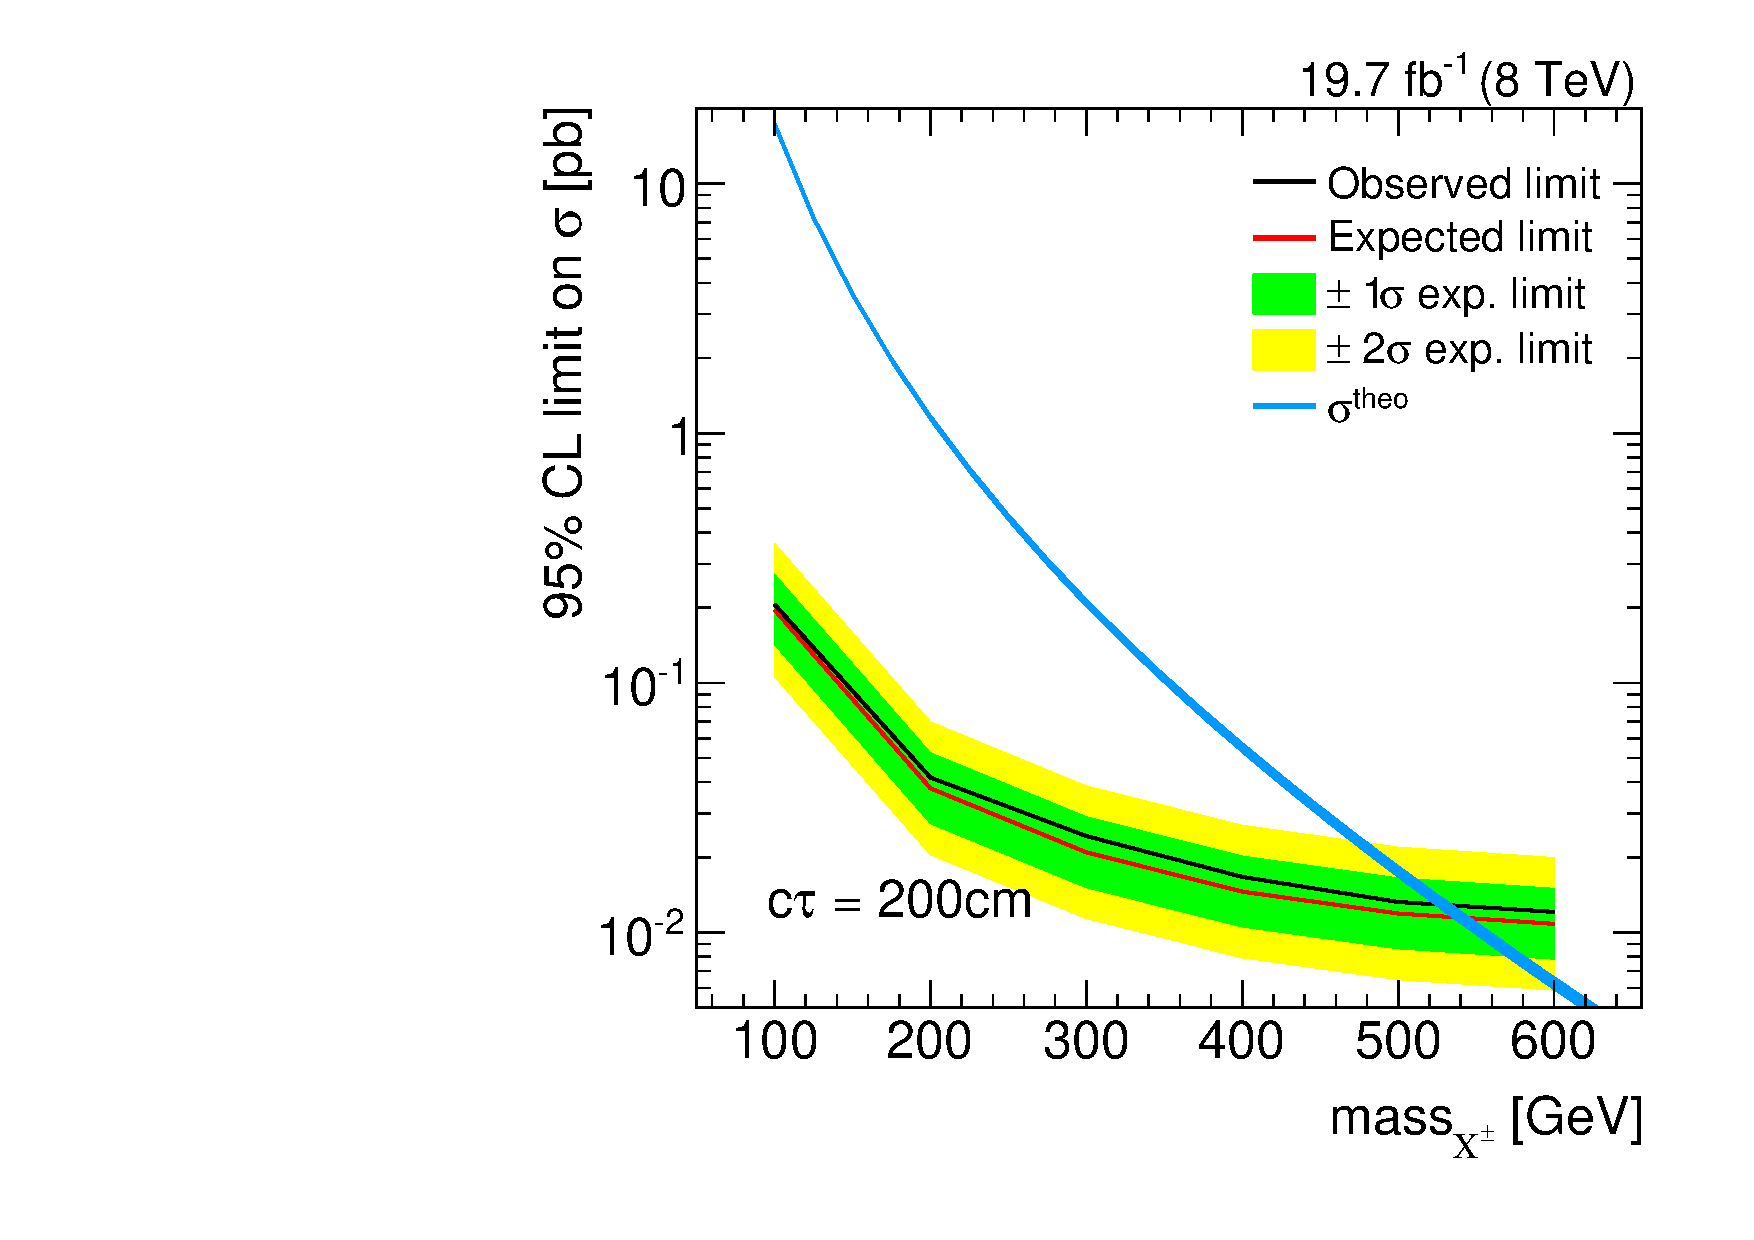
\includegraphics[width=0.29\textwidth]{figures/analysis/Interpretation/ExclusionLimits/LimitPlot_ctau200cm.pdf} 
    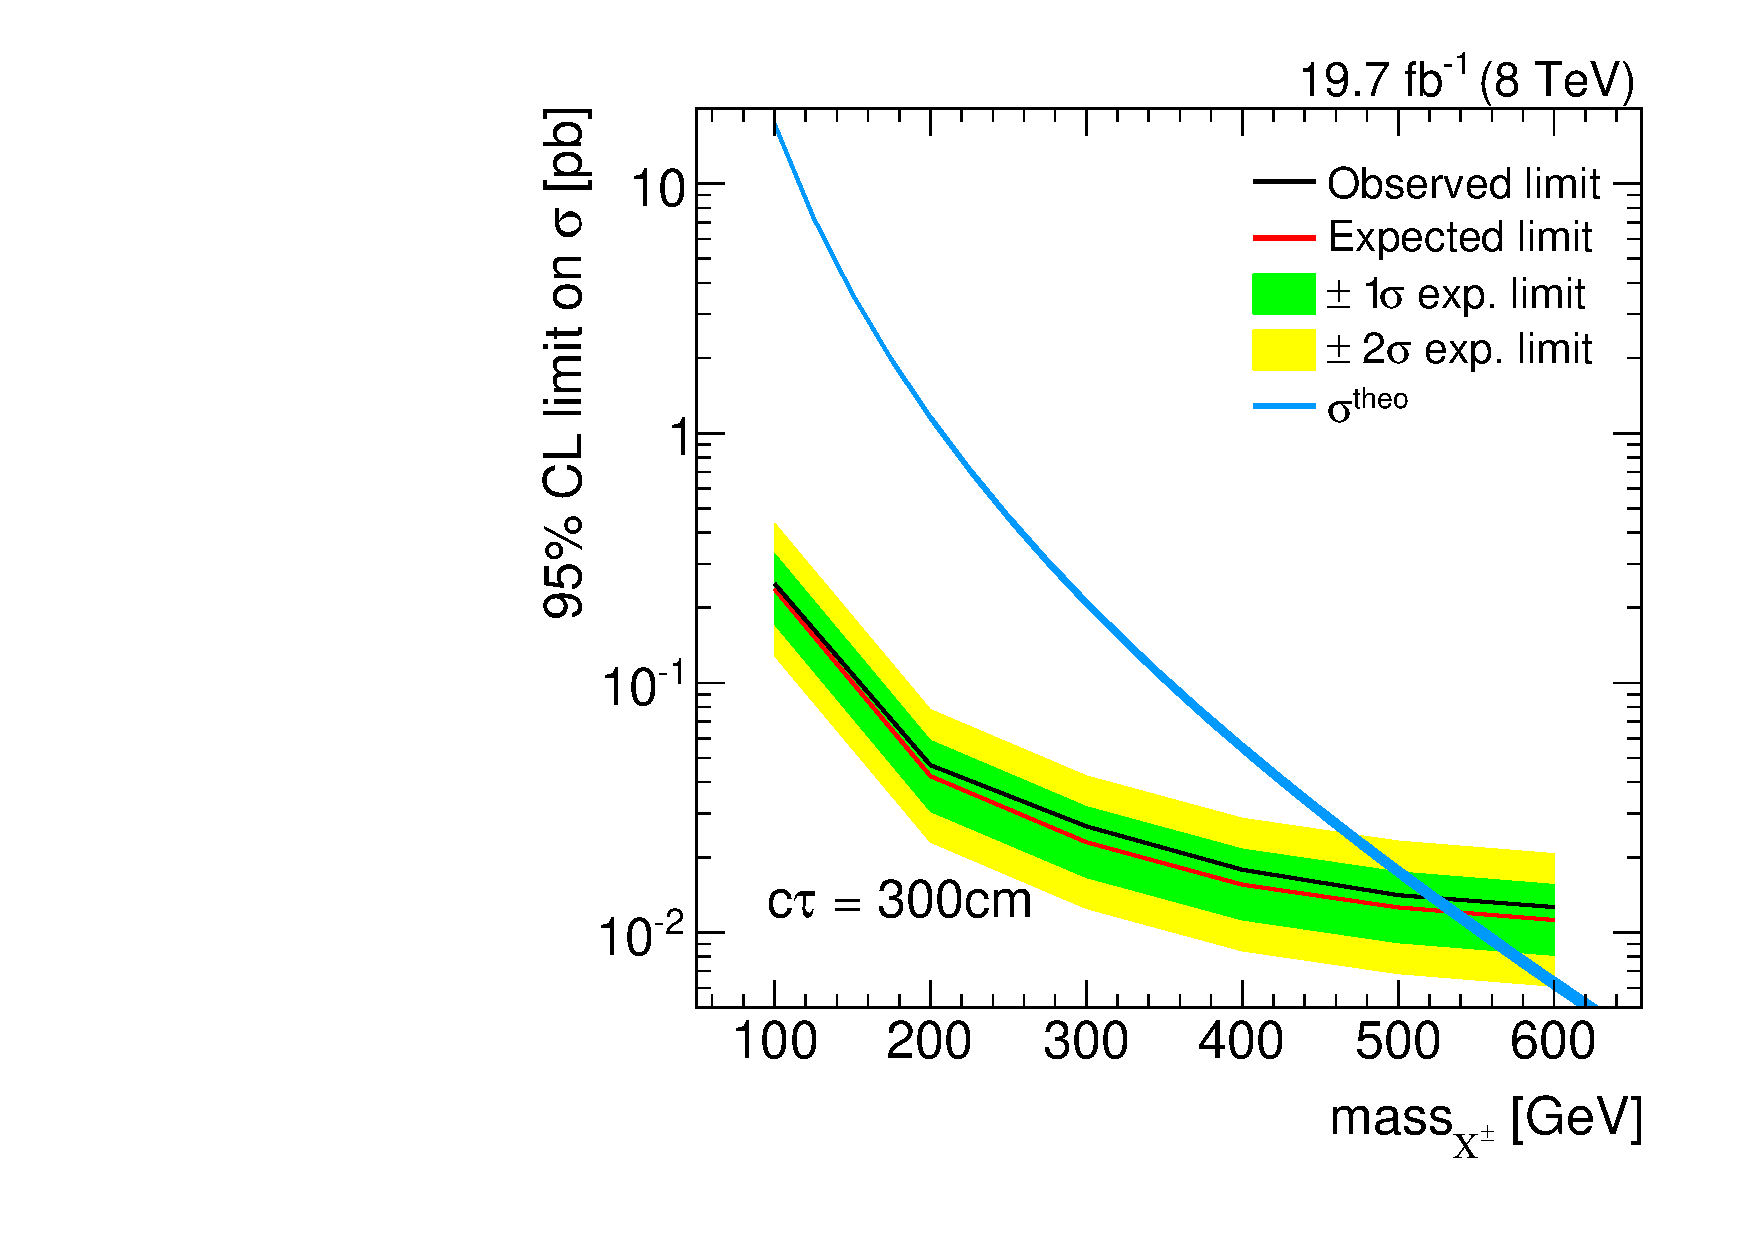
\includegraphics[width=0.29\textwidth]{figures/analysis/Interpretation/ExclusionLimits/LimitPlot_ctau300cm.pdf} \\
    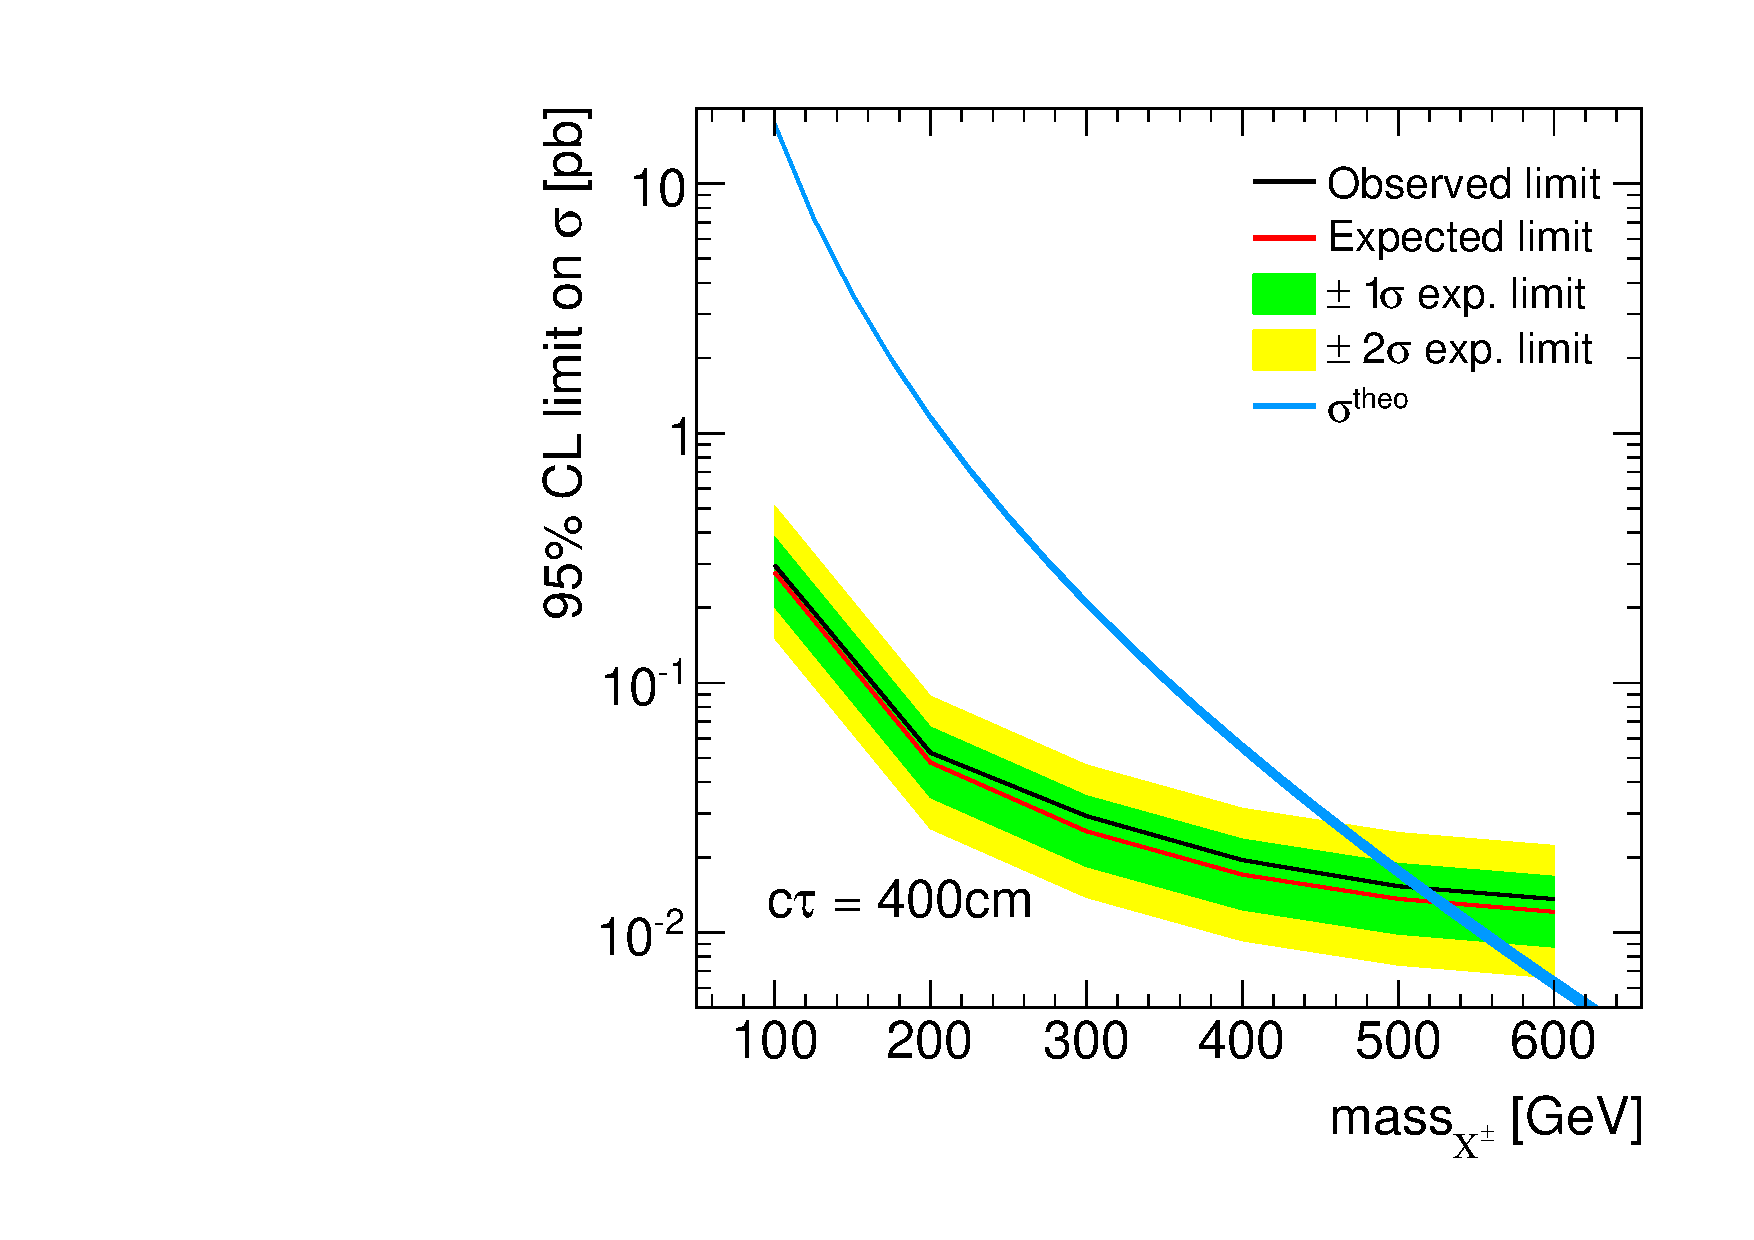
\includegraphics[width=0.29\textwidth]{figures/analysis/Interpretation/ExclusionLimits/LimitPlot_ctau400cm.pdf} 
    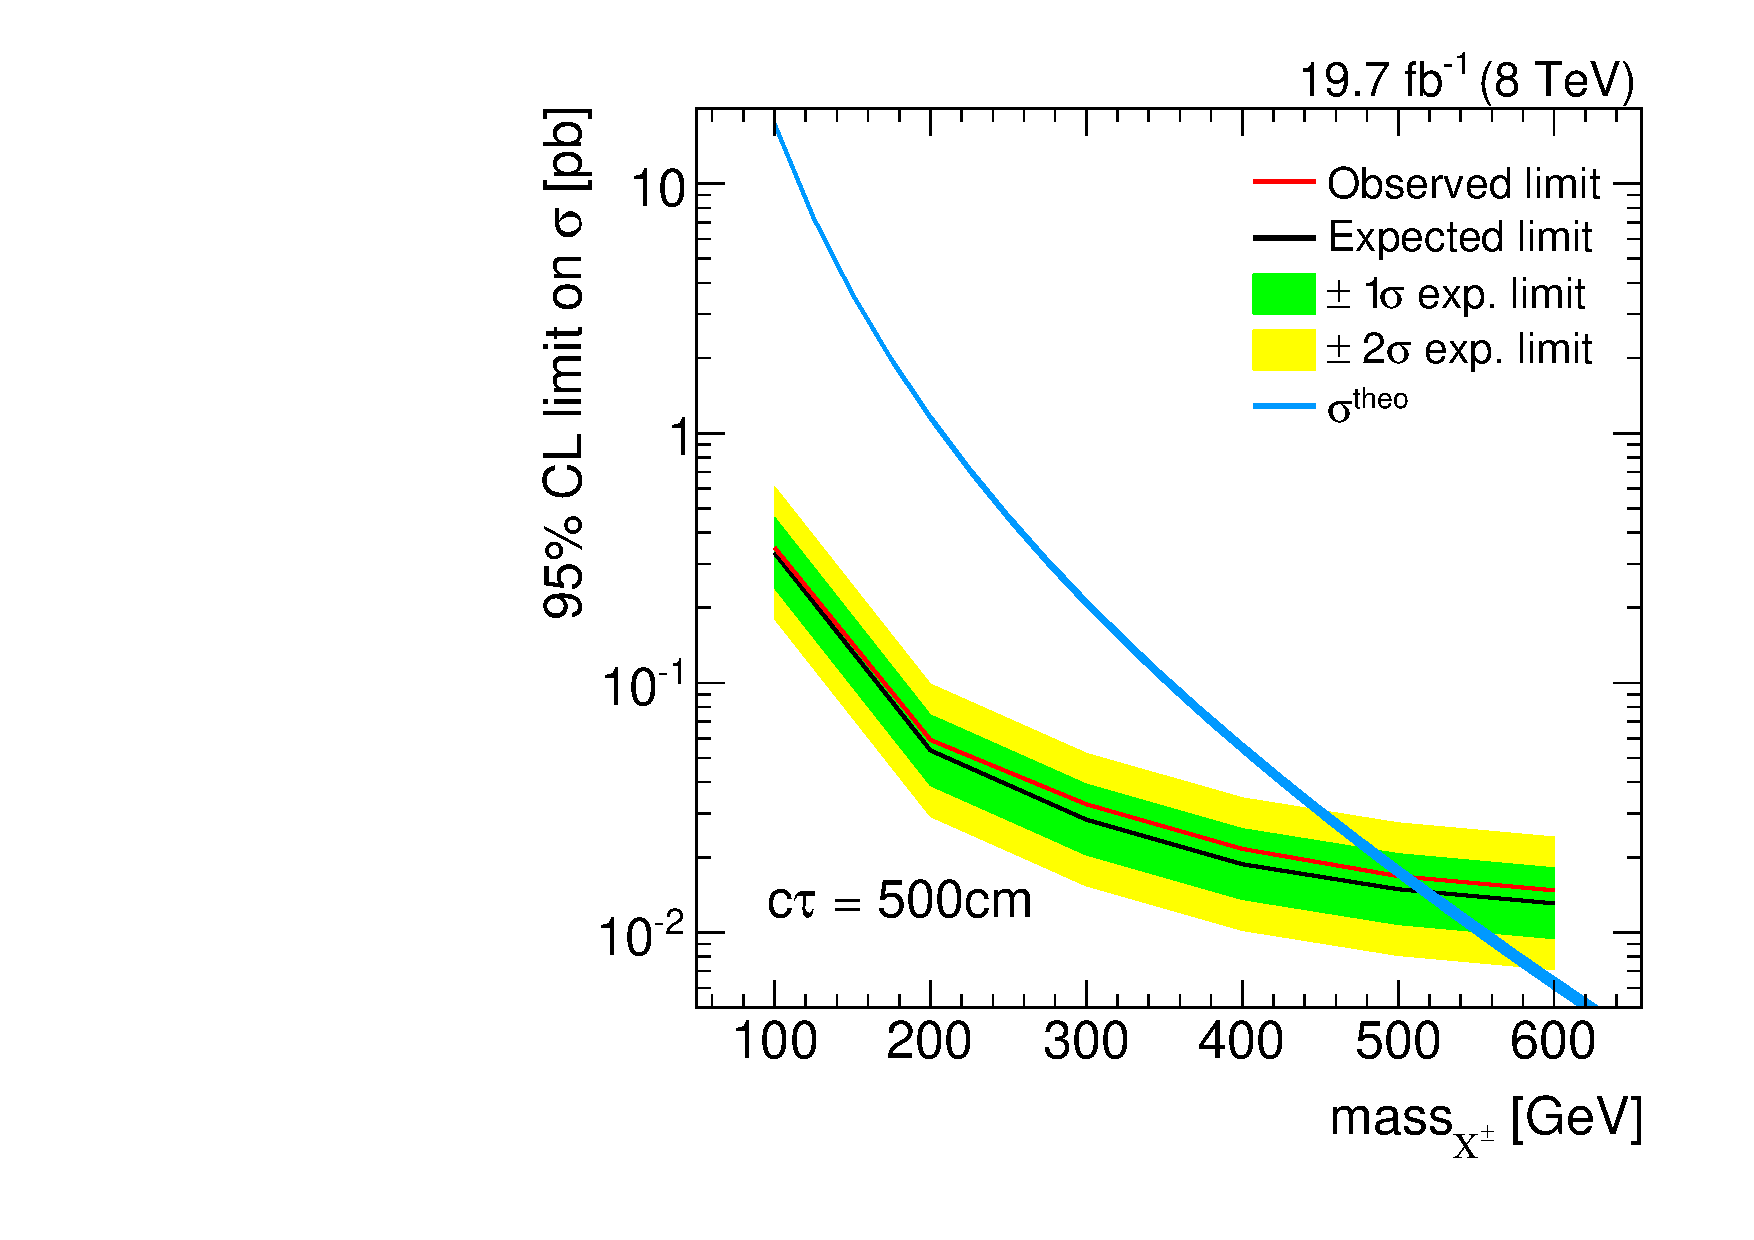
\includegraphics[width=0.29\textwidth]{figures/analysis/Interpretation/ExclusionLimits/LimitPlot_ctau500cm.pdf} 
    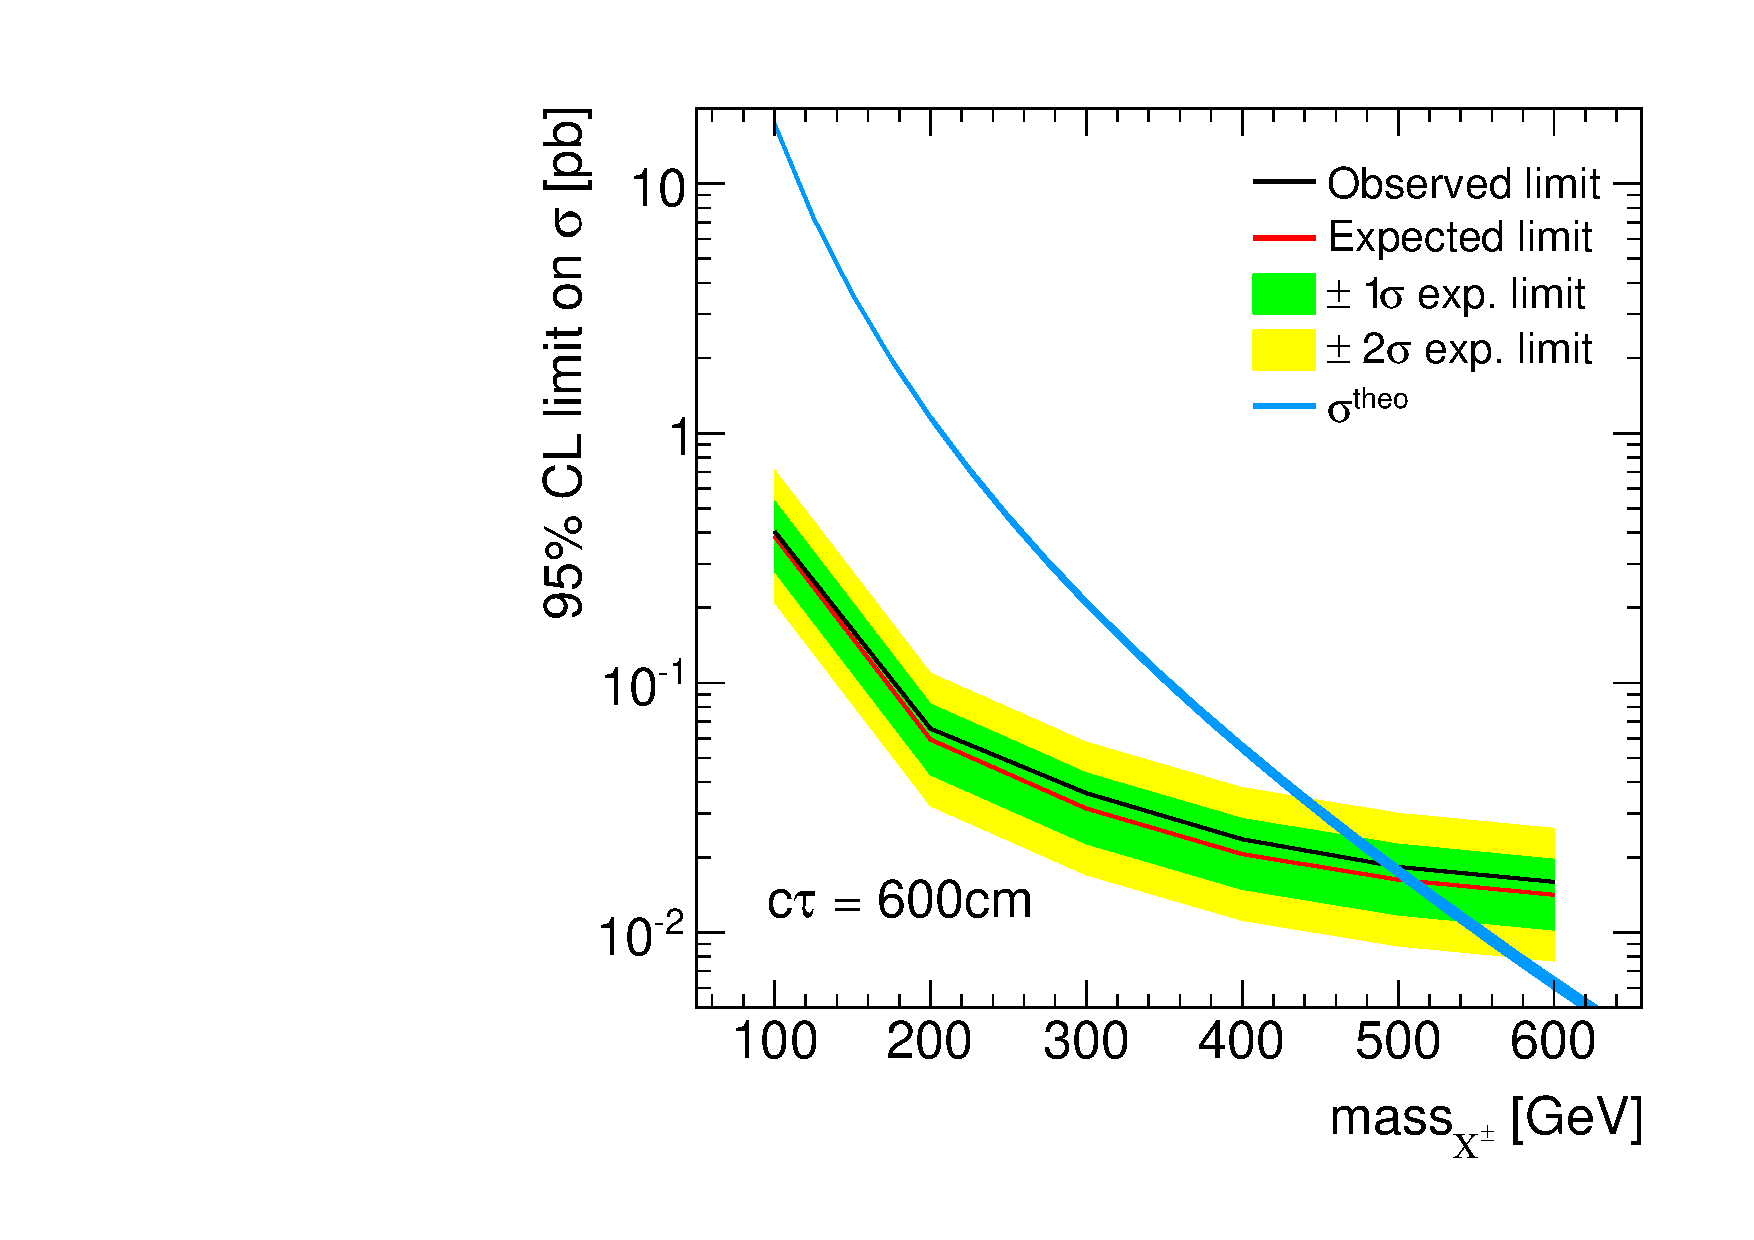
\includegraphics[width=0.29\textwidth]{figures/analysis/Interpretation/ExclusionLimits/LimitPlot_ctau600cm.pdf} \\
  \end{tabular}
  \caption{95\% CL exclusion limits for signal models with $\ctau = 40-600\cm$.}
  \label{fig:1dLimitsB}
\end{figure} 

\begin{figure}[!h]
  \centering 
  \begin{tabular}{c}
    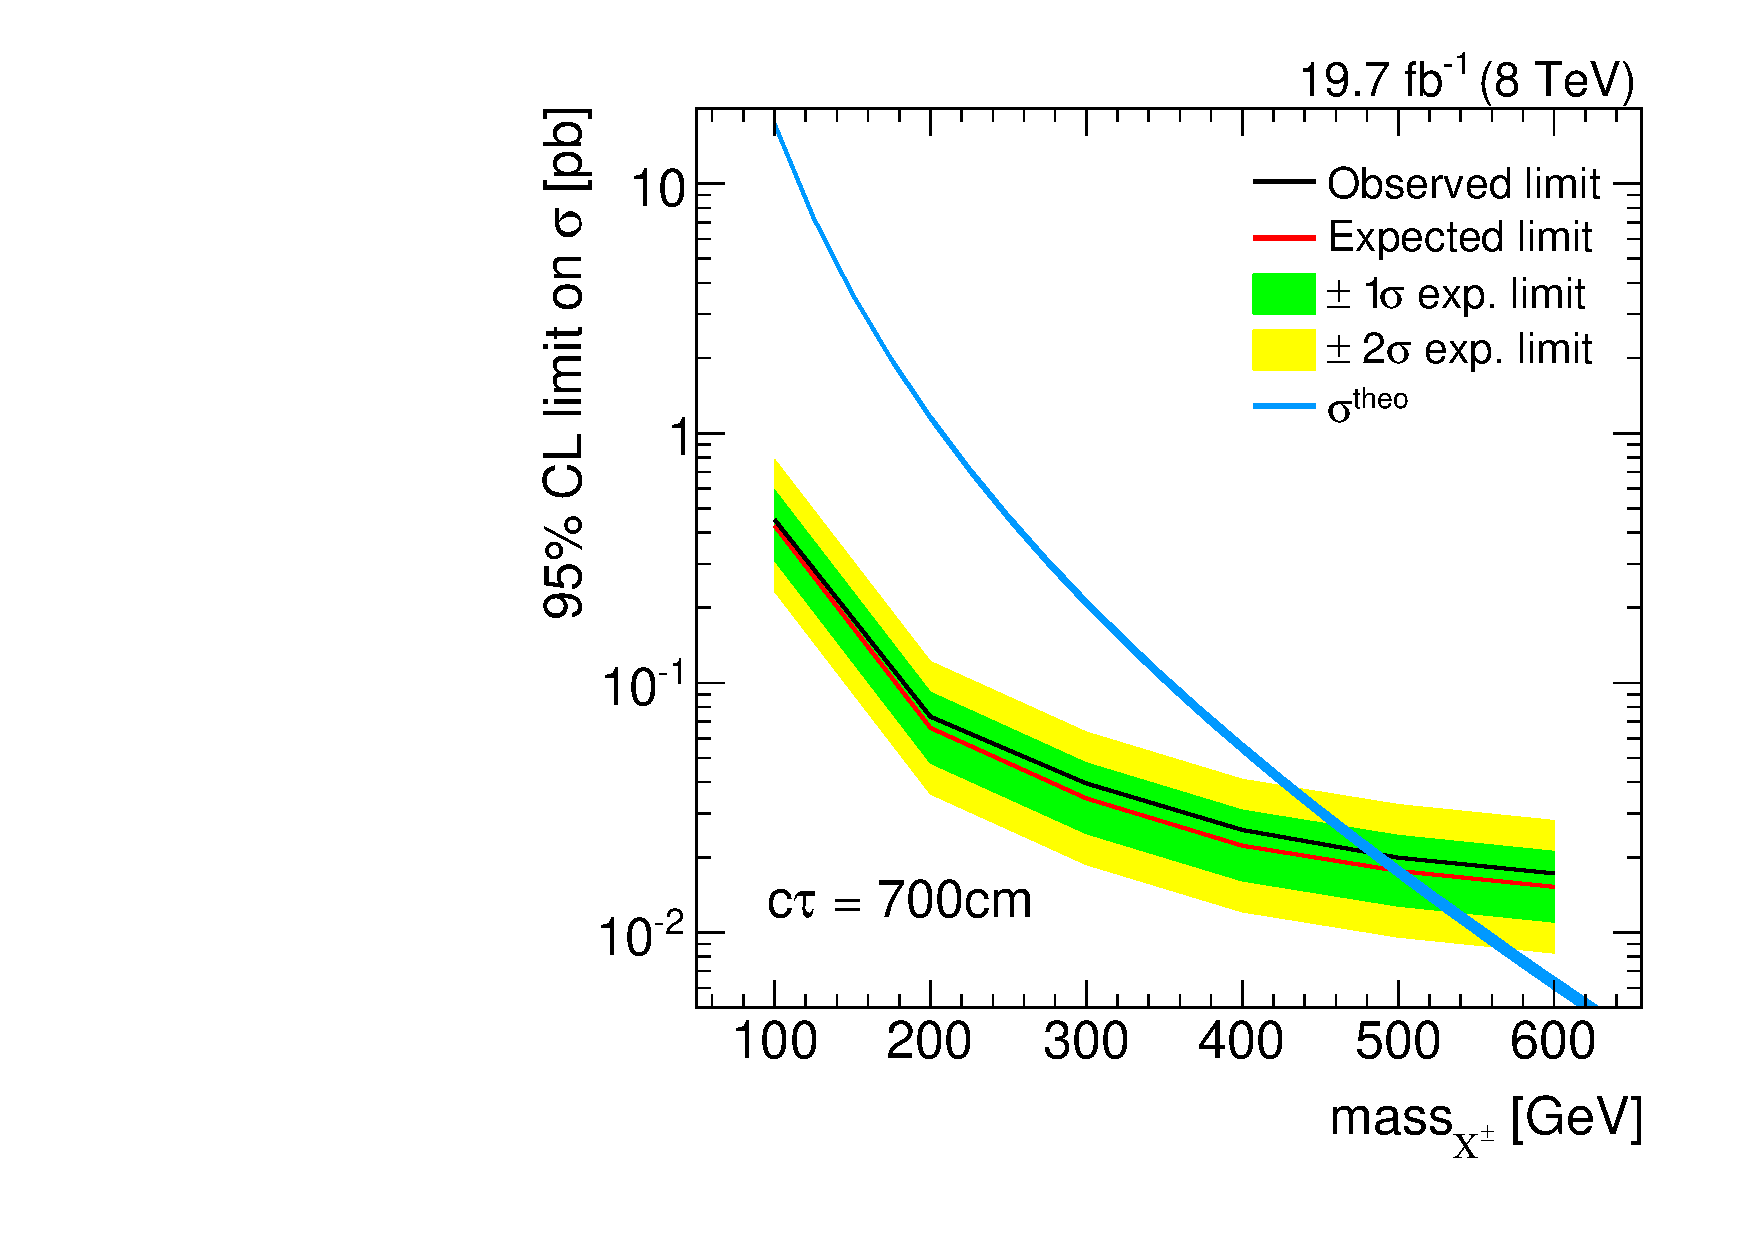
\includegraphics[width=0.29\textwidth]{figures/analysis/Interpretation/ExclusionLimits/LimitPlot_ctau700cm.pdf} 
    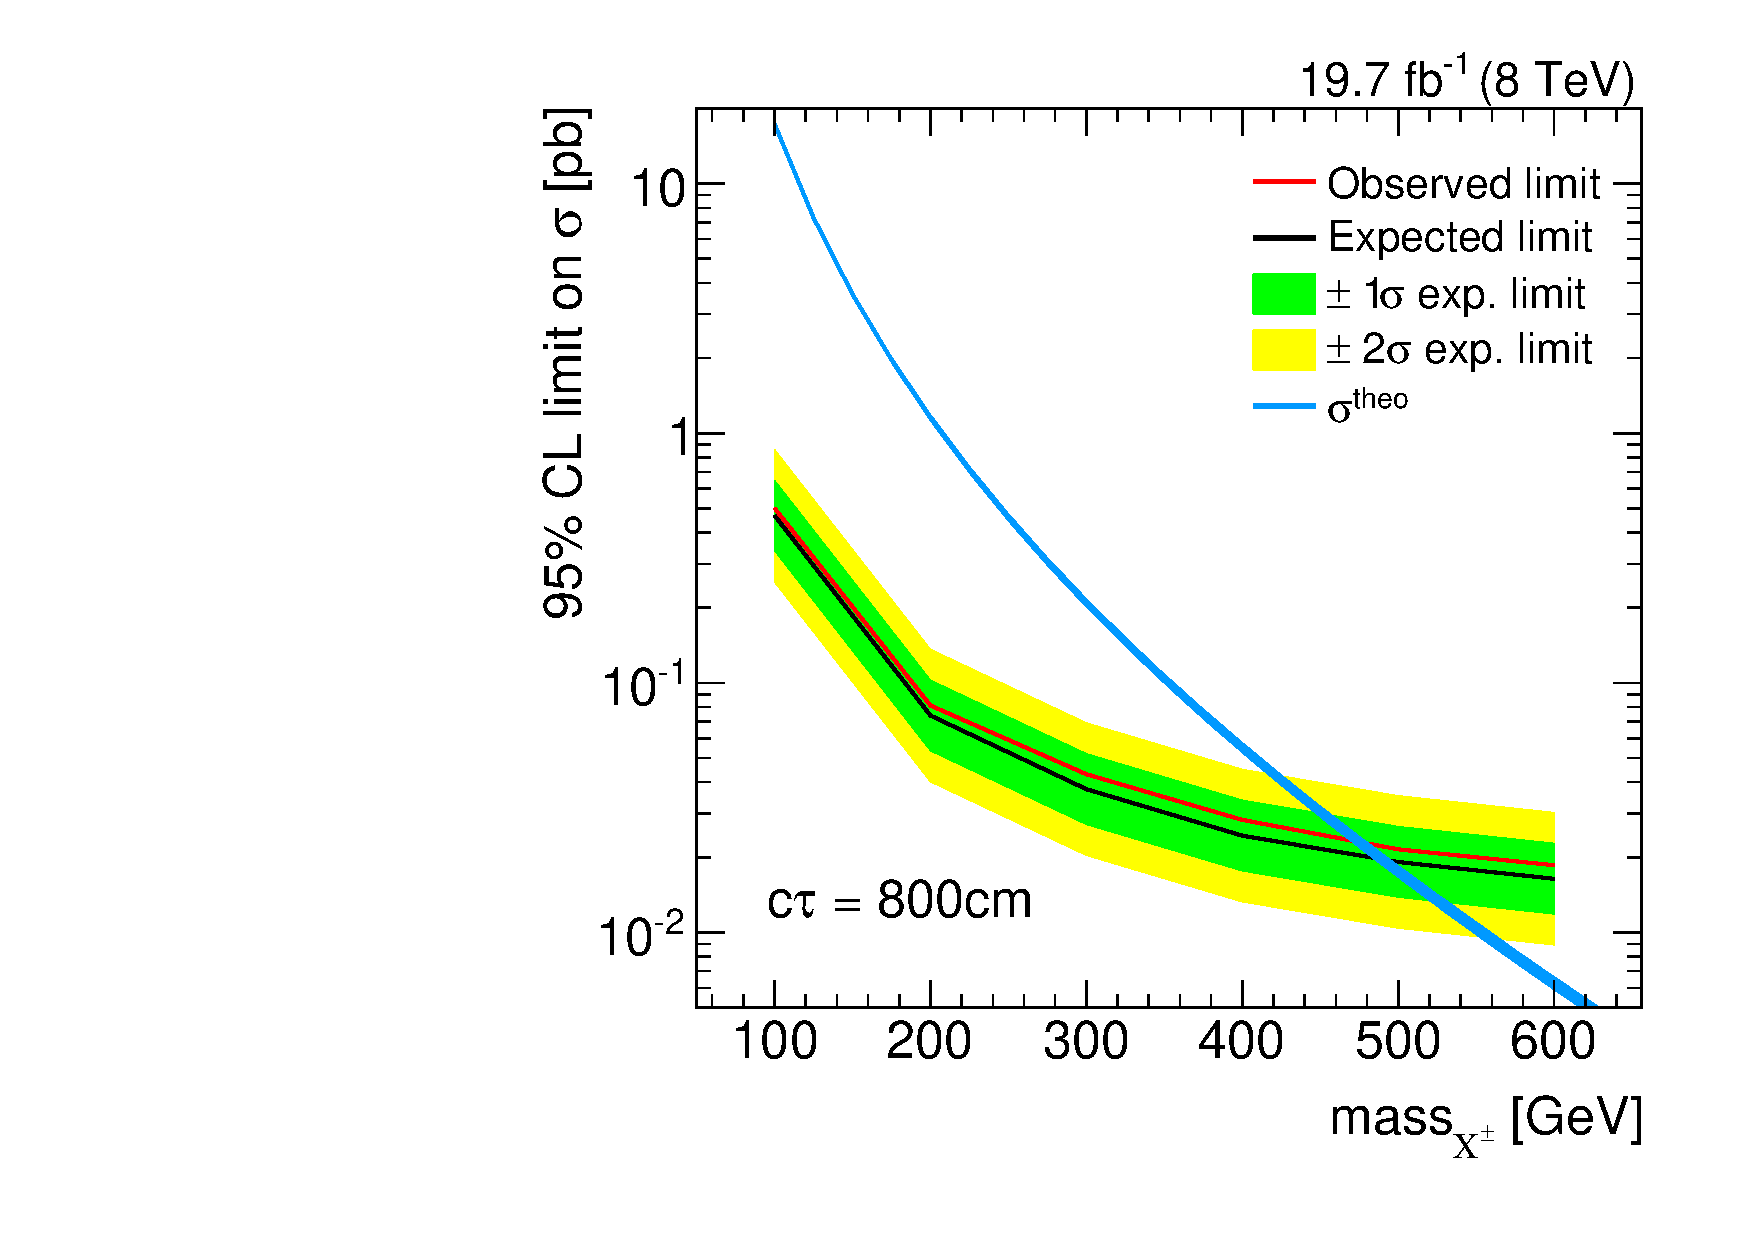
\includegraphics[width=0.29\textwidth]{figures/analysis/Interpretation/ExclusionLimits/LimitPlot_ctau800cm.pdf} 
    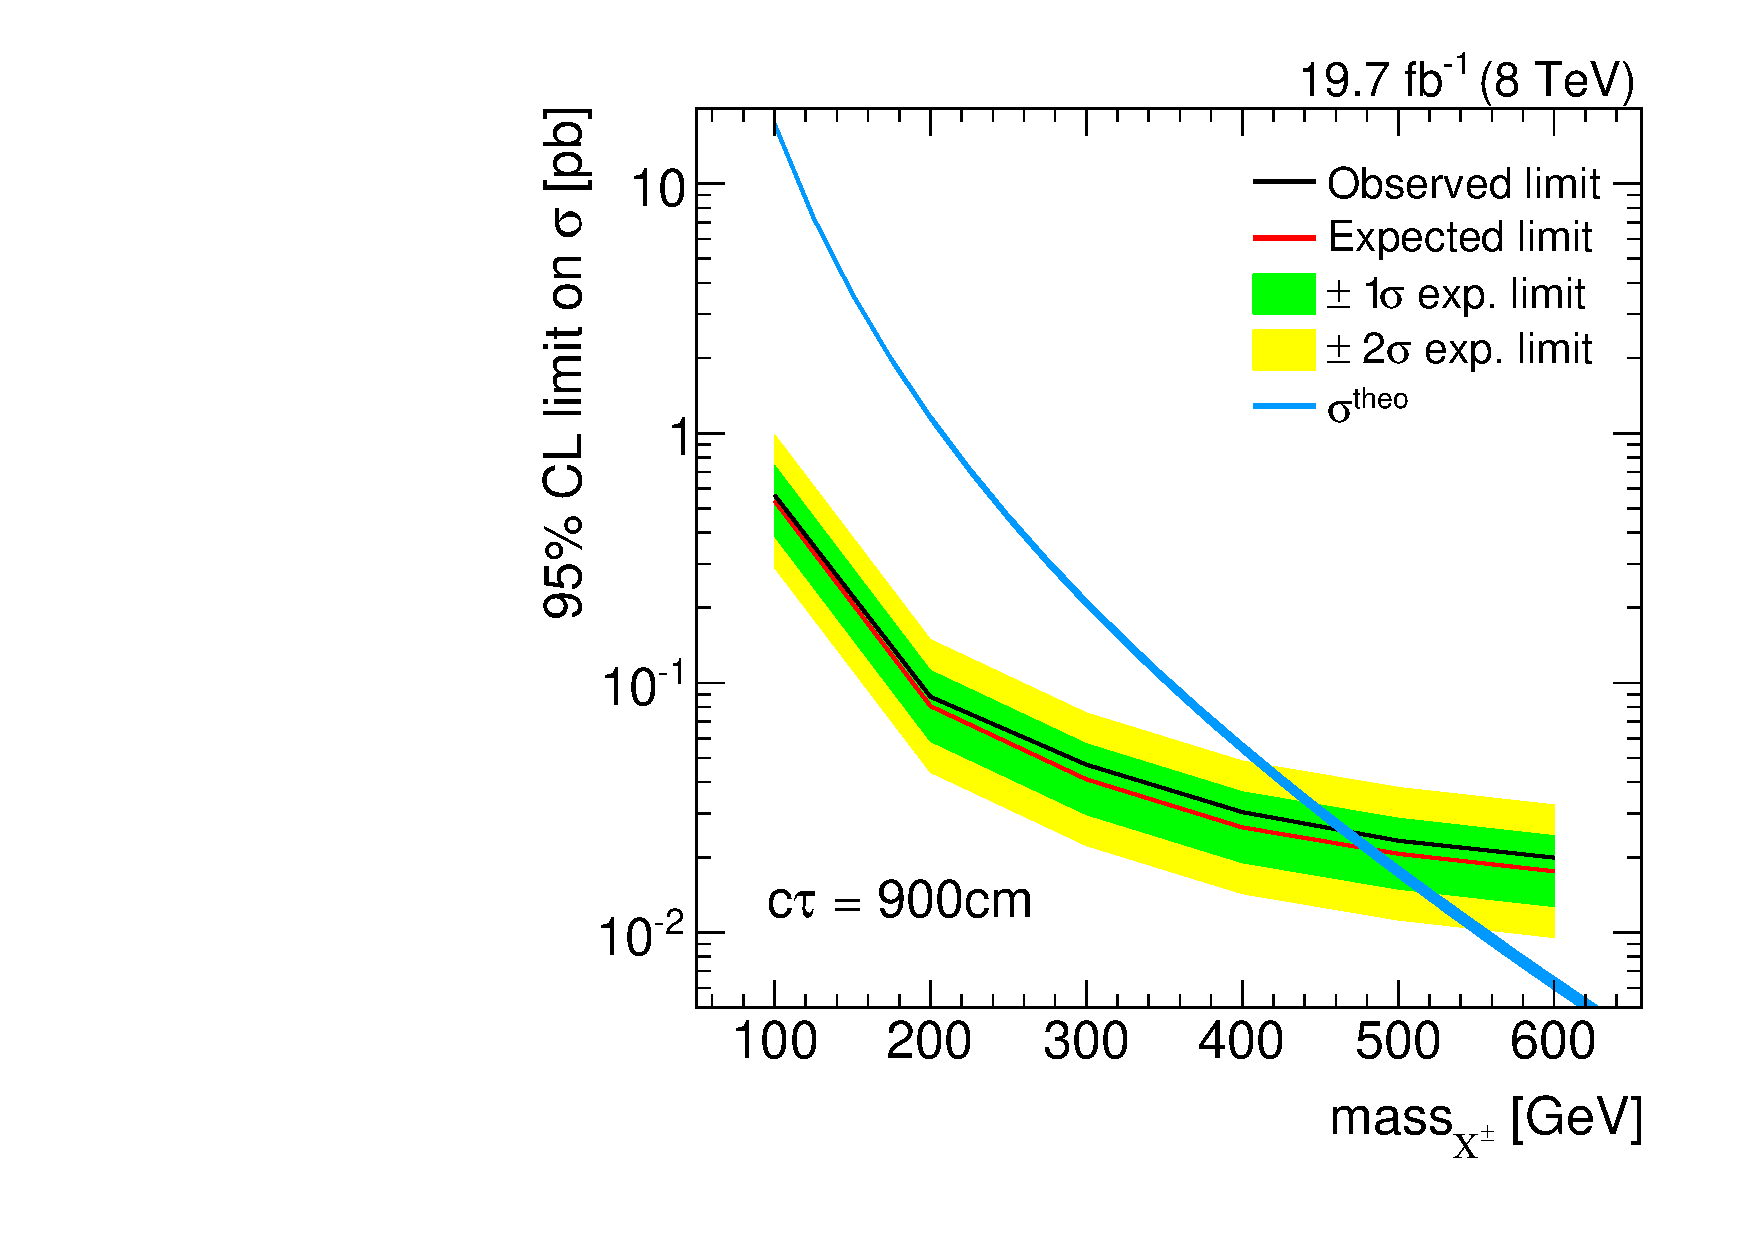
\includegraphics[width=0.29\textwidth]{figures/analysis/Interpretation/ExclusionLimits/LimitPlot_ctau900cm.pdf} \\
    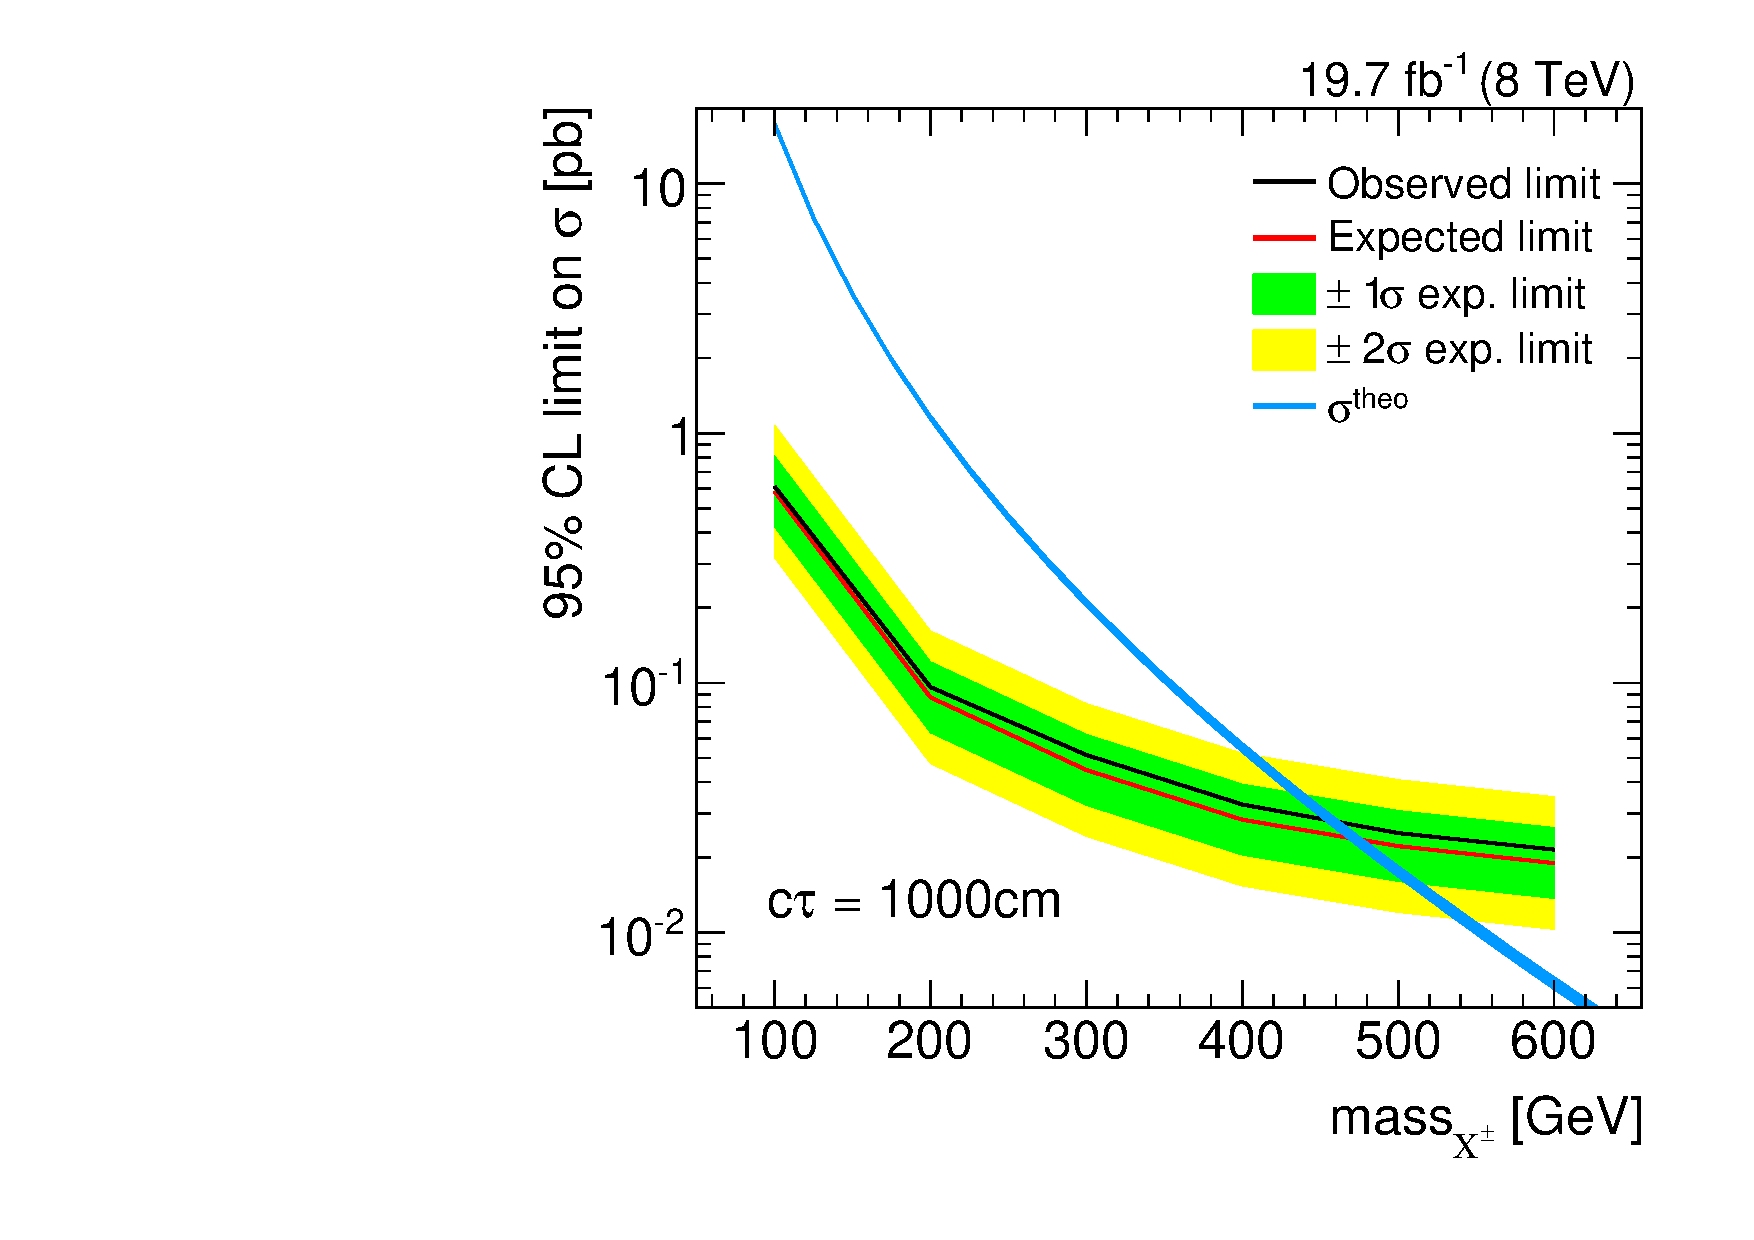
\includegraphics[width=0.29\textwidth]{figures/analysis/Interpretation/ExclusionLimits/LimitPlot_ctau1000cm.pdf} 
    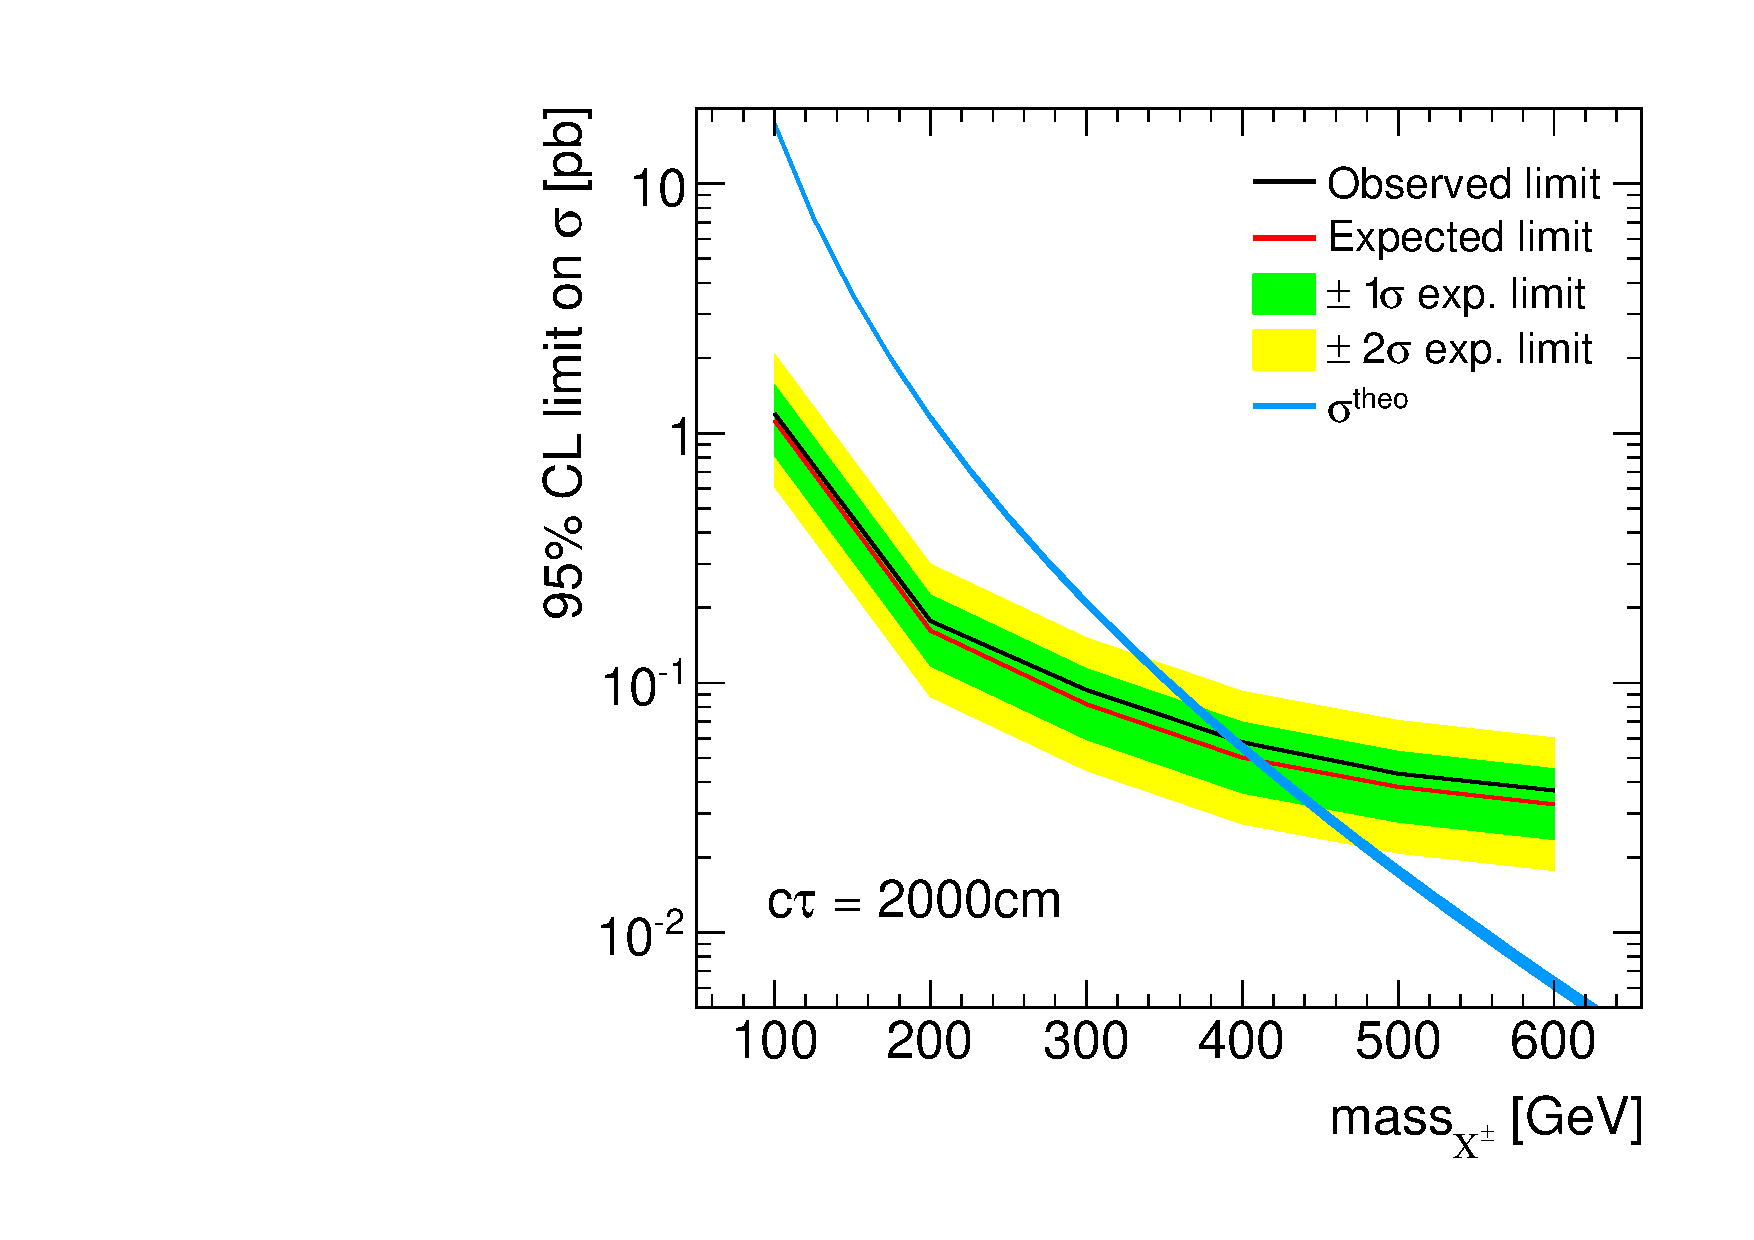
\includegraphics[width=0.29\textwidth]{figures/analysis/Interpretation/ExclusionLimits/LimitPlot_ctau2000cm.pdf} 
    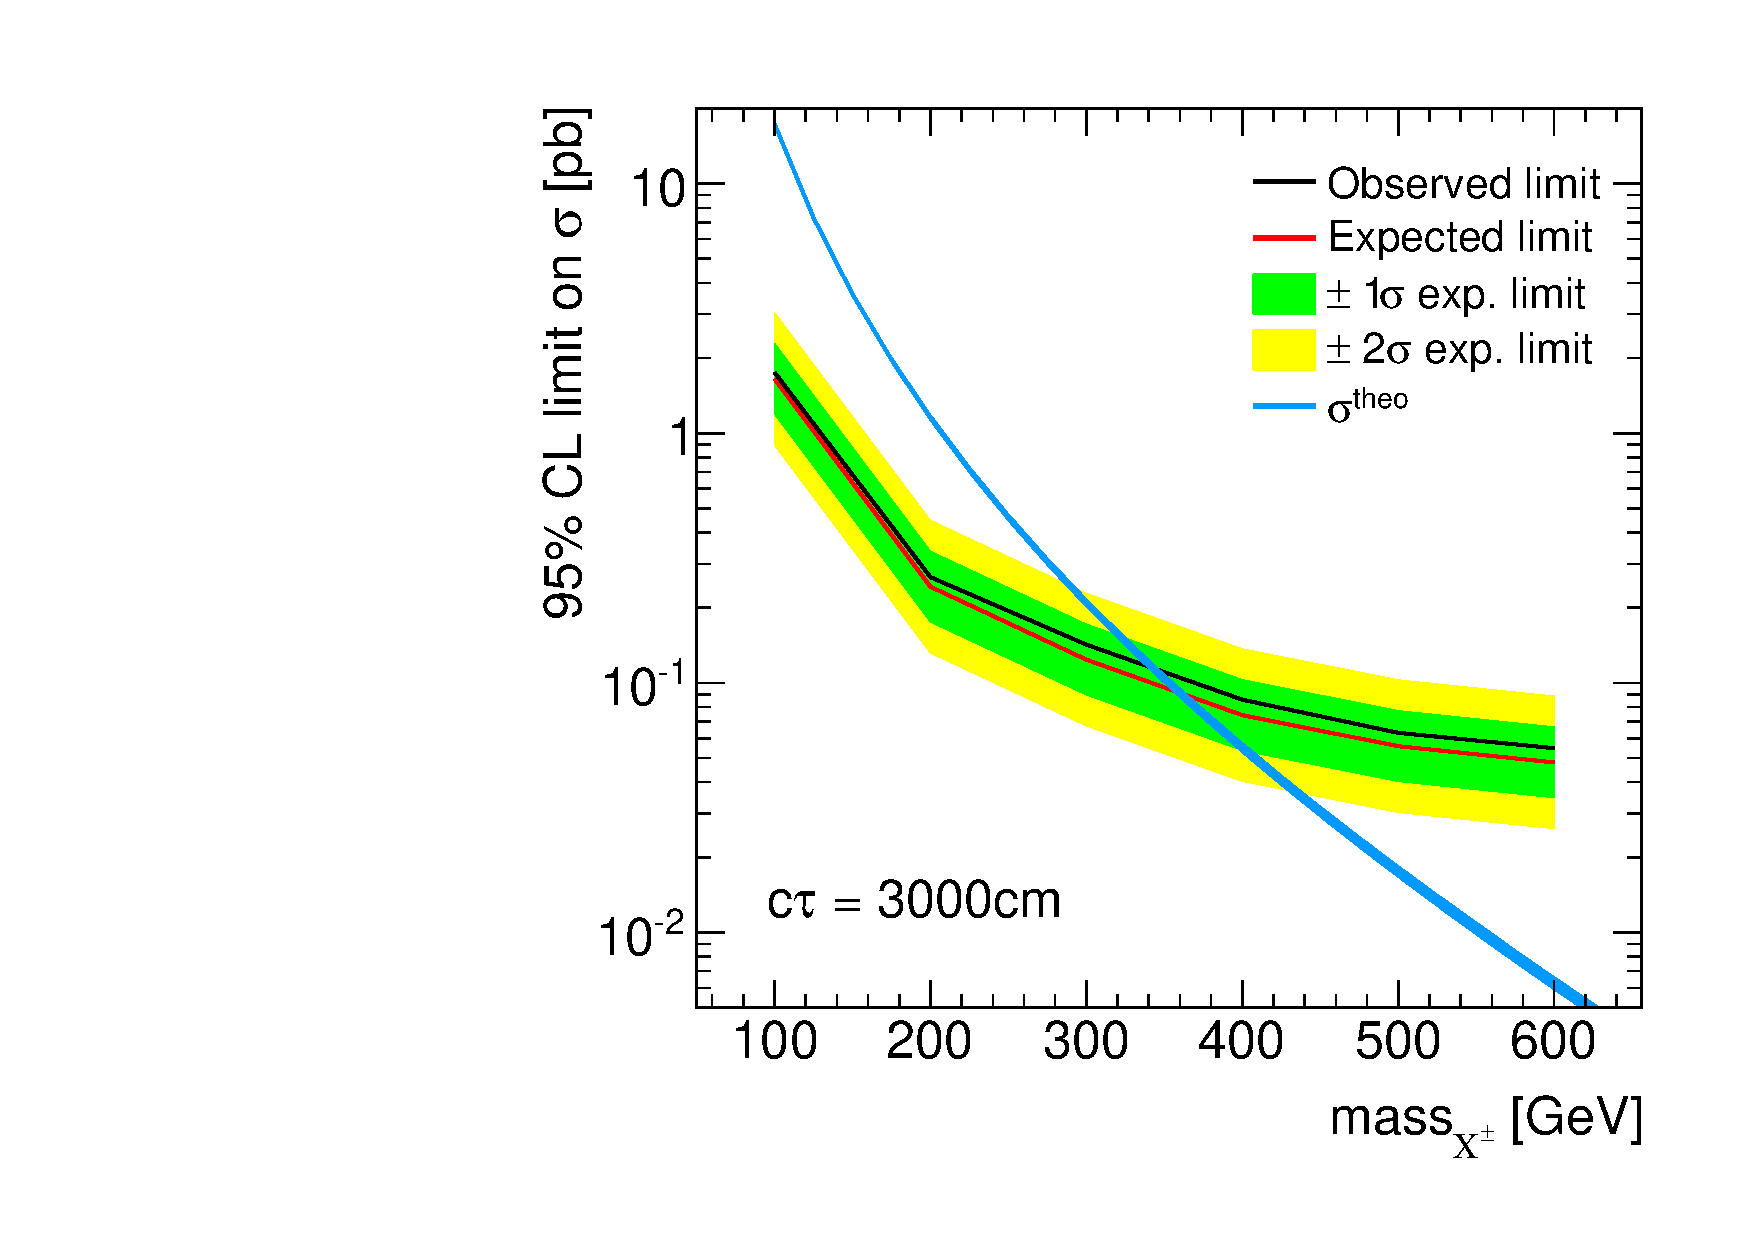
\includegraphics[width=0.29\textwidth]{figures/analysis/Interpretation/ExclusionLimits/LimitPlot_ctau3000cm.pdf} \\
    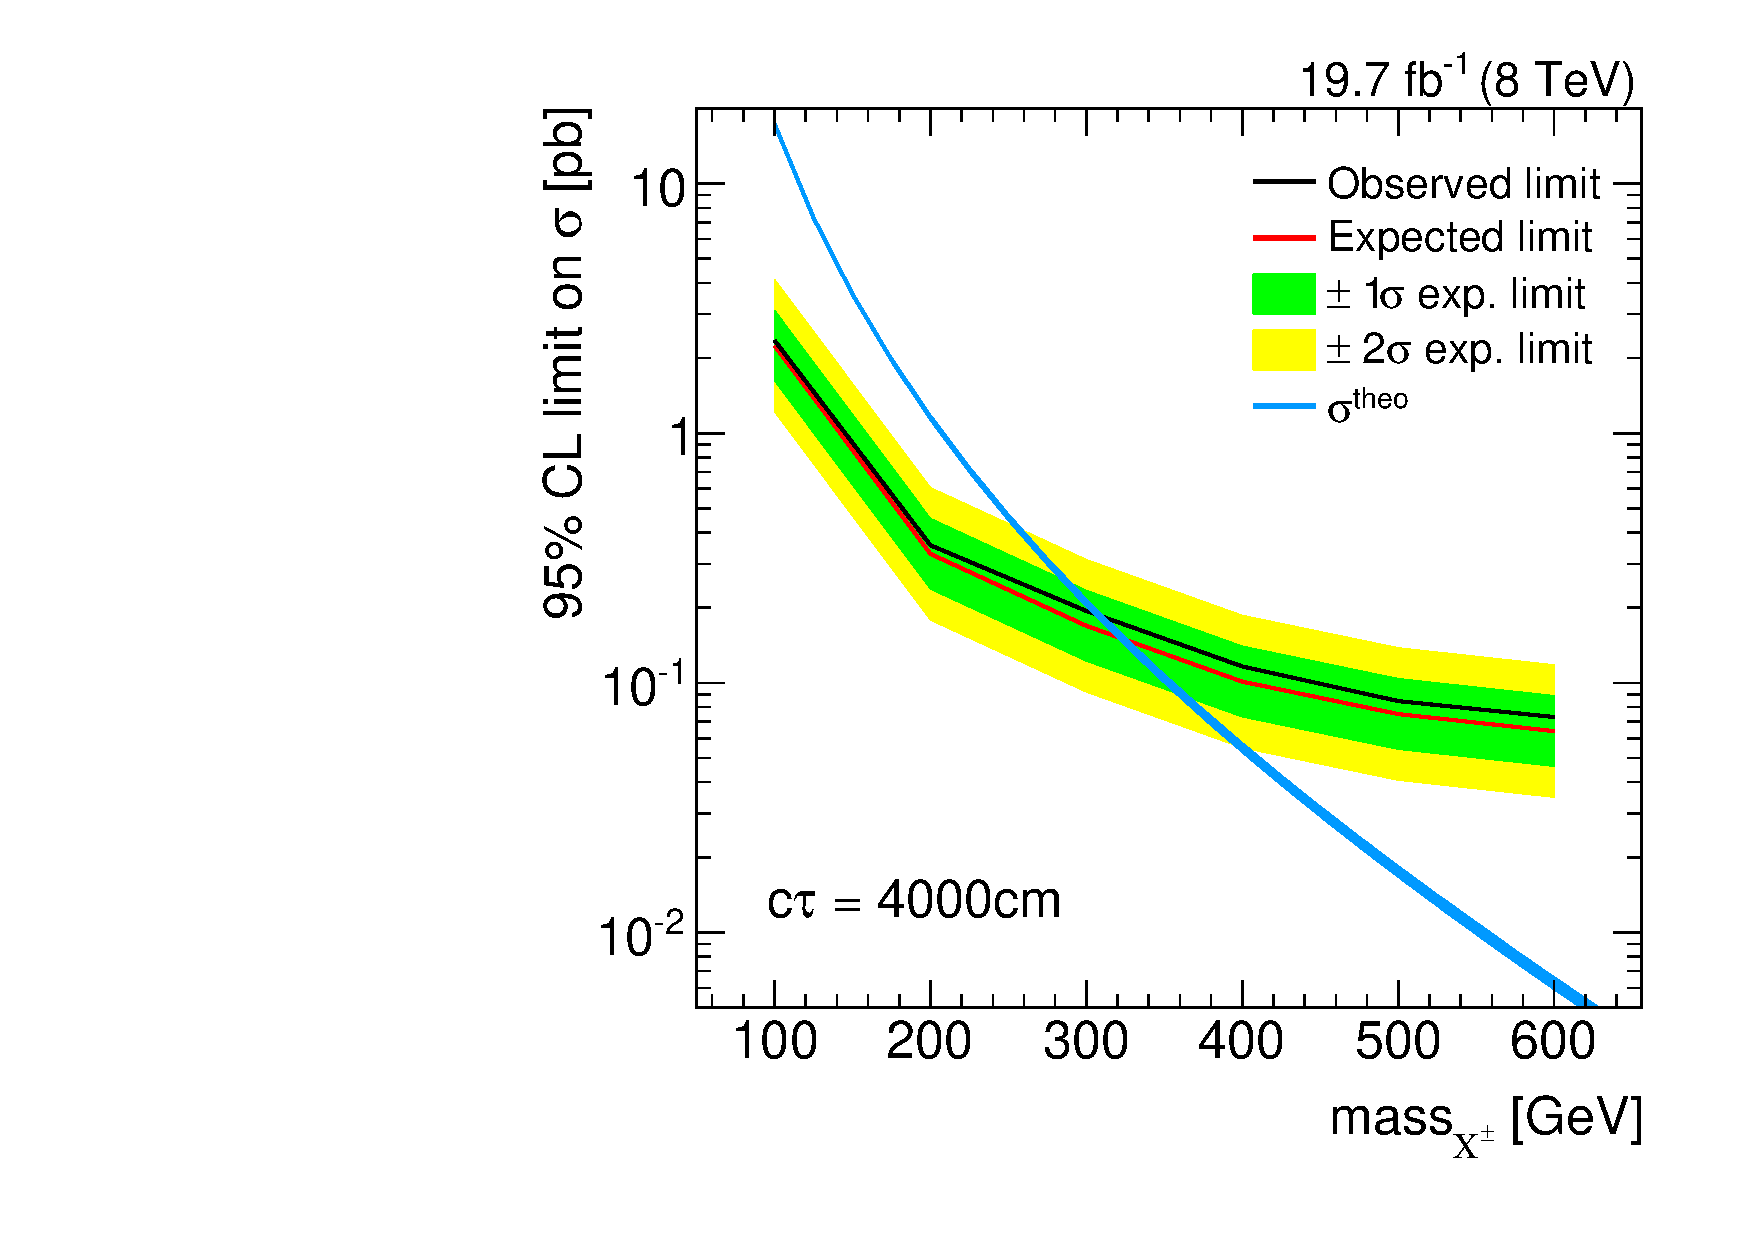
\includegraphics[width=0.29\textwidth]{figures/analysis/Interpretation/ExclusionLimits/LimitPlot_ctau4000cm.pdf} 
    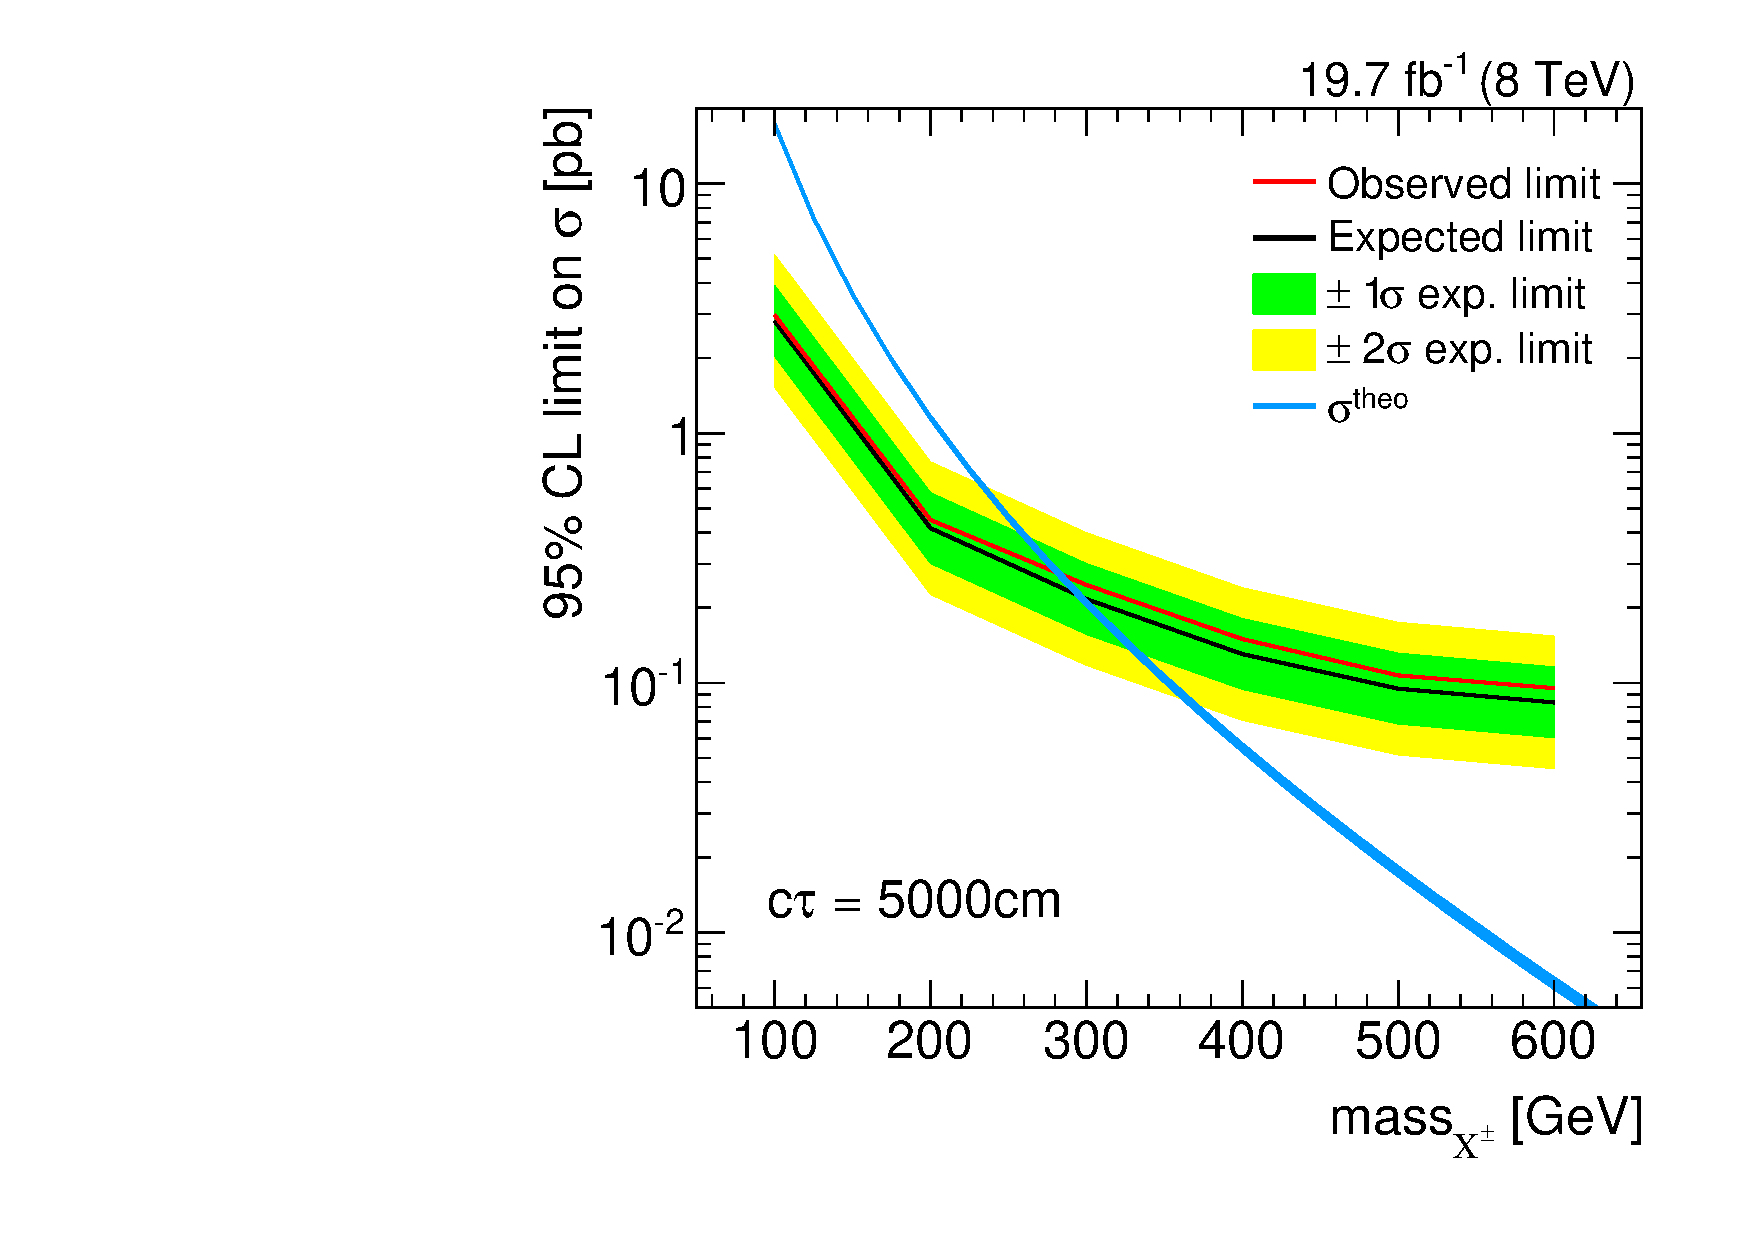
\includegraphics[width=0.29\textwidth]{figures/analysis/Interpretation/ExclusionLimits/LimitPlot_ctau5000cm.pdf} 
    \includegraphics[width=0.29\textwidth]{figures/analysis/Interpretation/ExclusionLimits/LimitPlot_ctau6000cm.pdf} \\
    \includegraphics[width=0.29\textwidth]{figures/analysis/Interpretation/ExclusionLimits/LimitPlot_ctau7000cm.pdf} 
    \includegraphics[width=0.29\textwidth]{figures/analysis/Interpretation/ExclusionLimits/LimitPlot_ctau8000cm.pdf} 
    \includegraphics[width=0.29\textwidth]{figures/analysis/Interpretation/ExclusionLimits/LimitPlot_ctau9000cm.pdf} \\
  \end{tabular}
  \caption{95\% CL exclusion limits for signal models with $\ctau = 700-9000\cm$.}
  \label{fig:1dLimitsC}
\end{figure} 
